\documentclass{article}
\usepackage{amsmath}
\usepackage{amssymb}
\usepackage[a4paper, top=25mm, bottom=25mm, left=25mm, right=25mm]{geometry}
\usepackage{pgfplots}
\usepackage{mathtools}
\usepackage[utf8]{inputenc}
\usepackage{cancel}
\pgfplotsset{compat=1.18}
\usepgfplotslibrary{polar}
\usepgfplotslibrary{fillbetween}

\begin{document}

\vspace*{\fill}
\begin{center}
\Huge 
\textbf{Hacettepe University}\\[1em]
\textbf{Mathematics II}\\
\textbf{Exam Solutions Manual}
\end{center}
\vspace*{\fill}
\newpage
\large
{\Large \textbf{1. Introduction}}

\hfill

\noindent Dear math learners, this document comprises the midterm and final exams of the course \textit{Mathematics I} with the code \textit{MAT123}. A sample of each preserved exam held in the past has been gathered from students in the Department of Electrical and Electronics Engineering. The exams are categorized into two main exams: Midterms and Finals. Every midterm exam is identified as a \textit{Midterm} exam, whereas the \textit{Final}, \textit{Resit}, and \textit{Makeup} exams are considered to be final exams throughout the document. The solutions are checked through various platforms, including \textit{Desmos}, \textit{GeoGebra}, and \textit{WolframAlpha}.

\hfill

\noindent Should you find a mistake with the solution or need consultation, please get in touch with the author via the following:

\hfill

\textbf{Author's name}: Baturay Kafkas

\textbf{Author's email:} baturaykafkas@hacettepe.edu.tr

\textbf{Author's personal email}: kfksbtry@gmail.com

\hfill

\hfill

{\Large \textbf{2. Motivation}}

\begin{itemize}
\item To help learners understand the fundamentals of calculus,
\item To make students have the knowledge of mathematical symbols and notations,
\item To help students prepare for exams with proper writing skills,
\item To make students gain ideas for advanced math courses,
\item To help students have expertise in academic writing.
\end{itemize}

\hfill

{\Large \textbf{3. Exams and Solutions}}

\hfill

\noindent There are a total of $8$ midterm exams and $12$ final exams.

{\small\[
\begin{array}{c|c|c|c}
\text{Exam}&\text{Date}&\begin{array}{cc}
\text{Content}\\\text{Page}
\end{array}&\begin{array}{cc}
\text{Solution}\\\text{Page}
\end{array}\\\hline
\text{Midterm}&28/03/2012&4&29\\
\text{Midterm}&08/06/2020&5&33\\
\text{Midterm}&15/08/2020&7&37\\
\text{Midterm}&28/04/2021&8&41\\
\text{Midterm}&20/04/2022&9&46\\
\text{Midterm}&08/05/2023&10&50\\
\text{Midterm}&26/04/2024&11&55\\
\text{Midterm}&09/04/2025&12&60\\
\end{array}\quad\begin{array}{c|c|c|c}
\text{Exam}&\text{Date}&\begin{array}{cc}
\text{Content}\\\text{Page}
\end{array}&\begin{array}{cc}
\text{Solution}\\\text{Page}
\end{array}\\\hline
\text{Final}&01/07/2020&14&67\\
\text{Resit}&01/07/2020&15&71\\
\text{Final}&28/08/2020&16&78\\
\text{Final}&09/06/2021&17&82\\
\text{Final}&23/05/2022&18&86\\
\text{Final}&12/06/2023&19&91\\
\text{Makeup}&12/06/2023&20&96\\
\text{Final}&11/01/2024&21&101\\
\text{Resit}&29/01/2024&23&107\\
\text{Final}&04/06/2024&25&113\\
\text{Makeup}&27/06/2024&26&118\\
\text{Final}&18/06/2025&27&121
\end{array}\]}
\newpage


\vspace*{\fill}
\begin{center}
\Huge \textbf{MIDTERMS}
\end{center}
\vspace*{\fill}
\newpage


\begin{center}
2011-2012 Spring \\MAT124 Midterm I\\(28/03/2012)\\Time: 13:00 - 15:00\\Duration: 120 minutes
\end{center}

\noindent 1. Consider the curve with the polar equations $r=2-2\sin\theta$.

\hfill

(a) Sketch this curve.

\hfill

(b) Find the area of the region enclosed by this curve.

\hfill

(c) Find the tangent vector(s) to this curve at $\displaystyle\theta=\frac\pi4$.

\hfill

\noindent 2. Consider the points $A(0,-1,1),\:B(-1,0,1),\:C(1,0,2),\:D(0,0,1)$  in $\mathbb{R}^3$.

\hfill

(a) Find the equation of the plane passing through $A, B$ and $C$.

\hfill

(b) Find the distance from the point $D$ to the plane passing through $A, B$ and $C$.

\hfill

(c) Find the equation of the line passing through $B$ and $D$.

\hfill

\noindent 3. Consider the space curve whose vector equation is given by

\[r(t)=\mathrm{e}^t\sin t\,\mathbf{i}+\mathrm{e}^t\cos t\,\mathbf{j}+\mathrm{e}^t\,\mathbf{k} \quad\text{for}\quad 0\leq t\leq1\,.\]

\hfill

(a) Sketch the curve.

\hfill

(a) Find the length of the curve.

\hfill

\noindent 4. Evaluate the limit, if it exists, and explain your answer.

\hfill

(a) $\displaystyle \lim_{(x,y)\to(-1,-2)}\frac{y+2}{x^2y-xy+2x^2-2x}$ \ \ \ (b) $\displaystyle\lim_{(x,y)\to(0,0)}\frac{4x^2y}{x^4+y^2}$

\hfill

\hfill

\noindent 5. Answer each independent question below.

\hfill

(a) Let $f(x,y)=\ln\left(x^2+y^2\right)$. Evaluate $f_{xx}+f_{yy}$.

\hfill

(b) Sketch the surface given by $z=2x^2+y^2+4y+6$.

\newpage



\begin{center}
2019-2020 Spring \\MAT124 Midterm\\(08/06/2020)
\end{center}

\noindent 1. Find an equation for the line $L$ that contains the point $P= (-1,3,1)$ and is orthogonal to the line

\[\frac{x-2}{-1}=\frac{y-1}{-2}=\frac{z-5}{1}=\lambda,\quad\lambda\in\mathbb{R}\]

\hfill

\noindent 2. Sketch the graph of the following surfaces.

\hfill

(a) $z=\mathrm e^y$ \ \ \ (b) $y=z^2-x^2$

\hfill

\noindent 3. The position vector for a particle in space is given as

\[\textbf{R}(t) = (2\cos t)\textbf{i}+t^2\textbf{j}+(2\sin t)\textbf{k}.\]
    
\noindent Find the velocity and acceleration vectors of the particle and find the speed and direction of motion at t = $\pi/2$.

\hfill

\noindent 4. Let $f$ be a function defined by

\[
f(x,y) =
\left.
\begin{cases}
\dfrac{xy^3}{x^2+y^6},&\text{if}\, (x, y)\neq (0,0)\\[1em]0,&\text{if}\,(x,y)=(0,0).
\end{cases}
\right.
\]

\hfill

\noindent Is $f$ continuous at $(0,0)$? Explain.

\hfill

\noindent 5. Use the $\epsilon - \delta$ definition and show that the function

\[
f(x,y) =
\left.
\begin{cases}
\displaystyle \frac{x^2y}{x^2+y^6},&\text{if}\, (x, y)\neq (0,0)\\[1em]0,&\text{if}\,(x,y)=(0,0)
\end{cases}
\right.
\]

\hfill

\noindent is continuous at the origin.

\hfill

\noindent 6. Note that in Cartesian coordinates, the Cauchy-Riemann equations are

\[\frac{\partial u}{\partial x}=\frac{\partial v}{\partial y}\quad\text{and}\quad\frac{\partial u}{\partial y}=-\frac{\partial v}{\partial x}\]

\hfill

\noindent where $u=(x,y)$ and $v=v(x,y)$.

\hfill

\noindent Let $x=r\cos\theta$ and $y=r\sin\theta$. Show that the Cauchy-Riemann equations take the form

\[\frac{\partial u}{\partial r} = \frac{1}{r} \frac{\partial v}{\partial\theta} \quad\text{and}\quad\frac1r\frac{\partial u}{\partial\theta}=-\frac{\partial v}{\partial r}.\]

\newpage

\noindent 7. According to Poiseuille’s law, the resistance to the flow of blood offered by a cylindrical blood vessel of radius $r$ and length $x$ is

\[R(x,r) = \frac{cx}{r^4}\]

\hfill

\noindent for a constant $c > 0$. A certain blood vessel in the body is 8 cm long and has a radius of $2$ mm. Estimate the percent change in $R$ when $x$ is increased by $3\%$ and $r$ is decreased by $2\%$.

\hfill

\noindent 8. Find the critical points of $f(x, y)=-x^3+9x-4y^2$ and classify each point as a relative maximum, a relative minimum, or a saddle point.

\newpage



\begin{center}
2019-2020 Summer \\MAT124 Midterm\\(15/08/2020)
\end{center}

\noindent 1. Find an equation for the line $L$ passing through the point $P=(0,2,1)$ and is parallel to the line of intersection of the planes $x-y-1=0$ and $3x+z-3=0$.

\hfill

\noindent 2. Show that the vector $\mathbf{v}=\mathbf{i}+5\mathbf{j}+4\mathbf{k}$ is orthogonal to the line passing through the points $(1,2,1)$ and $(-1,0,4)$.

\hfill

\noindent 3. Sketch the graphs of the following surfaces.

\hfill

\noindent (a) $x=\mathrm{e}^y+1$

\hfill

\noindent (b) $z^2=x^2-y^2+1$

\hfill

\noindent 4. Show that the limit

\[\lim_{(x,y)\to(0,0)}\frac{x^5y^3}{x^7+y^{21/2}}\]

\hfill

\noindent does not exist.

\hfill

\noindent 5. Use the $\epsilon-\delta$ definition and show that the function $f(x,y)=6x^2+7y^2$ is continuous at the origin.

\hfill

\noindent 6. Find $\displaystyle\frac{\partial w}{\partial r}$, where $w=\mathrm{e}^{2x-y+3z^2}$ and $x=r+s-t,\:y=2r-3s,\:z=2\cos(rst)$.

\hfill

\noindent 7. The diameter of the base and the height of a closed right circular cylinder are measured, and measurement are known to have errors of at most $0.5$ cm. If the diameter and height are taken to be $4$ cm and $8$ cm, respectively, find the bounds for the propagated error in

\hfill

\noindent (a) the volume $V$ of the cylinder,

\hfill

\noindent (b) the surface area $S$ of the cylinder.

\hfill

\noindent 8. Find the slope of the line that is parallel to the $yz$-plane and tangent to the surface $y\ln z+z-2=0$ at the point $(1,0,2)$.

\hfill

\noindent 9. Find the equation for the tangent plane to the surface $z=\sin x+\mathrm{e}^{xy}+2y$ at the point $P=(0,1,3)$.

\newpage


\begin{center}
2020-2021 Spring \\MAT124 Midterm\\(28/04/2022)
\end{center}

\noindent 1. Consider the straight lines $\displaystyle x-1=\frac z3,\: y=0$ and $\displaystyle x=\frac{y+1}2=z$.

\hfill

\noindent (a) Show that the lines are skew.

\hfill

\noindent (b) Find an equation for the plane passing through the point $(1,3,5)$ which is parallel to the skew lines.

\hfill

\noindent 2. Sketch the graphs of the following surfaces in $\mathbb{R}^3$.

\hfill

\noindent (a) $z^2=y^2+x^2$

\hfill

\noindent (b) $z=y^3$

\hfill

\noindent 3. Let $C$ be the space curve given by the vector-valued function

\[\mathbf{R}(t)=(1+2\sin(2\pi t))\mathbf{i}+(\ln t)\mathbf{j}+(\cos(\pi t))\mathbf{k}\]

\hfill

\noindent Find an equation of the line which is tangent to $C$ at $\mathbf{R}(1)$.

\hfill

\noindent 4. Use the $\epsilon-\delta$ definition and show that the function

\[f(x,y)=\left\{\begin{array}{cl}
\displaystyle\frac{4x^2-y^2}{2x+y},& \text{if }(x,y)\neq(1,-2)\\[1em]
4,&\text{if }(x,y)=(1,-2)
\end{array}\right.\]

\hfill

\noindent is continuous at the point $(1,-2)$.

\hfill

\noindent 5. Calculate $\displaystyle\frac{\partial w}{\partial u}$ if $\displaystyle w=f(x,y,z)=\frac{x+\sin y}z$ and

\[x=x(u,v)=\ln(u+v),\quad y=y(u,v)=\mathrm{e}^{uv},\quad z=z(u,v)=\frac1u.\]

\hfill

\noindent 6. The opposite and adjacent sides of a base and the height of a right triangular prism are measured, and measurements are known to have errors of at most $0.4$ cm. If the opposite and adjacent sides of the base and the height are taken to be $5$ cm, $3$ cm, and $6$ cm, respectively, find the bounds for the propagated error in the volume of the triangular prism.

\hfill

\noindent 7. Find the maximum and minimum values of $f(x,y,z)=x-z$ on the ellipsoid

\[x^2+2y^2+z^2=1.\]

\hfill

\noindent 8. Find the critical points of $f(x,y)=x^3-y^3+xy$ and classify each point as a relative maximum, a relative minimum, or a saddle point.

\newpage


\begin{center}
2021-2022 Spring \\MAT124 Midterm\\(20/04/2022)
\end{center}

\noindent 1. Find the convergence set of the power series $\displaystyle\sum_{k=1}^\infty\frac{(\ln k)x^k}k$.

\hfill

\noindent 2. Show that the vectors $\mathbf{u}=\mathbf{i}+3\mathbf{j}+\mathbf{k},\:\mathbf{v}=2\mathbf{i}-\mathbf{j}-\mathbf{k}$, and $\mathbf{w}=7\mathbf{j}+3\mathbf{k}$ are coplanar (all in the same plane).

\hfill

\noindent 3. Find the point where the line

\[x-1=z,\:y=3\]

\hfill

\noindent intersects the plane $2y-z=5$.

\hfill

\noindent 4. Sketch the graphs of the following surfaces.

\hfill

\noindent (a) $z=\sin x$

\hfill

\noindent (b) $y=z^2-x^2$

\hfill

\noindent 5. Let $f$ be the function $\displaystyle f(x,y)=\frac{xy^2}{x^2+y^4}$ for $(x,y)\neq(0,0)$. Show that $f$ has no limit at $(0,0)$.

\hfill

\noindent 6. Van der Waal's equation in physical chemistry states that a gas occupying volume $V$ at temperature $T$ (Kelvin) exerts pressure $P$, where

\[\left(P+\frac A{V^2}\right)(V-B)=kT\]

\hfill

\noindent for physical constants $A, B$ and $k$. Compute the following rates.

\hfill

\noindent (a) the rate of change of volume with respect to temperature.

\hfill

\noindent (b) the rate of change of pressure with respect to volume.

\hfill

\noindent 7. Consider the surface $z=x^2+y^2-xy$, a paraboloid, on which a particle moves with $x$ and $y$ and coordinates given by $x=\cos t$ and $y=\sin t$. Using the chain rule, find $\displaystyle\frac{dz}{dt}$ when $t=0$. 

\hfill

\noindent 8. Find the parametric equations of the tangent line to the curve of intersection of the paraboloid $z=x^2+y^2$ and the ellipsoid $2x^2+2y^2+z^2=8$ at $P=(-1,1,2)$.

\newpage


\begin{center}
2022-2023 Spring \\MAT124 Midterm\\(08/05/2023)
\end{center}

\noindent 1. Sketch the traces of the following surfaces with the coordinate planes $x=0,\:y=0$, and $z=0$, and then sketch the graphs of them.

\hfill

\noindent (a) $\displaystyle\frac{x^2}{16}+\frac{y^2}4-z^2=1$

\hfill

\noindent (b) $\displaystyle z=\frac{x^2}4+\frac{y^2}4-6$

\hfill

\noindent 2. Show that the limit

\[\lim_{(x,y)\to(0,0)}\frac{y^3\sqrt x}{2\left(x^2+y^4\right)}\]

\hfill

\noindent does not exist.

\hfill

\noindent 3. Find the equation of the plane passing through the point $P_0(0,1,2)$ and which is perpendicular to the line that is tangent to the curve of intersection of the surfaces

\[xz^2-2xy+y^2=2\qquad\text{and}\qquad xz-x^2y+z^2=1\]

\hfill

\noindent at the point $P_1\left(0,\sqrt2, 1\right)$.

\hfill

\noindent 4. Find $\displaystyle\frac{\partial w}{\partial s}$ where $w=xy\ln\left(1+\sqrt{x^2+y^2}\right)+xz$ and $x=t+s,\:y=\mathrm{e}^s,\:z=\ln\left(s^2+t\right)$.

\hfill

\noindent 5. Use incremental approximation to estimate the value $\tan\left((0.97)\cdot(2.05)^2\right)$.

\hfill

\noindent 6. Find the direction vector in which the function

\[f(x,y,z)=\sqrt{x+yz}\]

\hfill

\noindent has the minimum rate of change at the point $(1,1,3)$. Also, find this rate of change.

\hfill


\noindent 7. Find the absolute extrema of

\[f(x,y)=x^2+y-xy+4\]

\hfill

\noindent on the triangular region with vertices $(0,0),\:(4,0),\:(0,4)$.

\newpage


\begin{center}
2023-2024 Spring \\MAT124 Midterm\\(26/04/2024)
\end{center}

\noindent 1. Sketch the traces of the following surfaces with the coordinate planes $x=0,\:y=0$, and $z=0$, and then sketch the graphs of them.

\hfill

\noindent (a) $y=\ln z$ \ \ \ (b) $x^2+2y^2-3z^2+1=0$

\hfill

\noindent 2. State the $\epsilon-\delta$ definition of the limit of a function of two variables, and using the $\epsilon-\delta$ definition, show that
\[\lim_{(x,y)\to(0,0)}\left(2x^2+y^2\right)=0\]

\hfill

\noindent 3. For $t\in\mathbb{R}$, let $l_1$ and $l_2$ be two lines given by

\[\begin{array}{ccccc}
x=3t&&&x=1+6\lambda&\\
y=4-t&t\in\mathbb{R}&& y=2-2\lambda&\lambda\in\mathbb{R}\\
z=1+2t&&\qquad&z=1+4\lambda&
\end{array}\]

\hfill

\noindent Determine an equation of the plane containing both $l_1$ and $l_2$.

\hfill

\noindent 4. Let
\[f(x,y)=\left\{\begin{array}{cc}
\displaystyle\frac{x^2\cdot\mathrm{e}^{x^2+y}}{x^2+y^2}&\text{if }(x,y)\neq(0,0)\\[1em]
0&\text{if }(x,y)=(0,0)
\end{array}\right.\]

\hfill

\noindent (i) Evaluate the partial derivatives $f_x(0,0)$ and $f_y(0,0)$.

\hfill

\noindent (ii) Show that $f(x,y)$ is not differentiable at $(0,0)$.

\hfill

\noindent 5. Let $u=u(x,y)$ and $v=v(x,y)$. The Cauchy-Riemann equations are

\[\frac{\partial u}{\partial x}=\frac{\partial v}{\partial y}\quad\text{and}\quad\frac{\partial u}{\partial y}=-\frac{\partial v}{\partial x}\]

\noindent Show that in the polar coordinate system $(x=r\cos\theta,\:y=r\sin\theta)$,

\[\frac{\partial u}{\partial r}=\frac1r\frac{\partial v}{\partial\theta}\quad\text{and}\quad\frac{\partial v}{\partial r}=-\frac1r\frac{\partial u}{\partial \theta}\]

\hfill

\noindent 6. Determine the direction at the point $(1,1)$ in which the rate of change of

\[f(x,y)=\frac{2^{xy}}x\]

\hfill

\noindent is the largest. Compute this rate of change.

\hfill

\noindent 7. Find all critical points of the function

\[f(x,y)=(x-1)(y+1)(x-y+3)\]

\hfill

\noindent and then determine whether each critical point corresponds to a local maximum, a local minimum or a saddle point.

\newpage


\begin{center}
2024-2025 Spring \\MAT124 Midterm\\(09/04/2025)
\end{center}

\noindent 1. Consider the curve with the polar equation $r=2\cos(3\theta)$.

\hfill

\noindent (a) Find symmetry properties for the given curve and sketch the curve.

\hfill

\noindent (b) Find the area of the region enclosed by the curve.

\hfill

\noindent 2. Identify (describe and sketch) the following curves with polar equations using Cartesian coordinates.

\hfill

\noindent (i) $r=2\sin\theta +2\cos\theta$ \ \ \ (ii) $r=\tan\theta\sec\theta$

\hfill

\noindent 3.

\hfill

\noindent (a) The following vectors are given.
\[\mathbf{u}=6\mathbf{i}-3\mathbf{j}+2\mathbf{k}\quad\text{and}\quad\mathbf{v}=(4\mathrm{p}+1)\mathbf{i}+(\mathrm{p}-2)\mathbf{j}+\mathbf{k}\]

\noindent $\mathrm{p}$ is a scalar constant. Find the value of $\mathrm{p}$ if

\hfill

\noindent I. $\mathbf{u}$ and $\mathbf{v}$ are perpendicular vectors. \ \ \ \ \ II. $\mathbf{u}$ and $\mathbf{v}$ are parallel vectors.

\hfill

\noindent (b) The points $A(5,1,3),\:B(3,1,5),\:C(5,3,5)$ are given. Show that the triangle $\triangle{ABC}$ is equilateral and find its area.

\hfill

\noindent (c) Find the intersection of the line $L$ and the plane $R$.

\hfill

\noindent 4.

\hfill

\noindent (a) Find an equation of the plane through the point $P(1,2,3)$ parallel to the plane $R: x+y+z=1$.

\hfill

\noindent (b) Find the parametric equations of a line $L$ through the point $P(1,2,3)$ and perpendicular to the plane $R$.

\hfill

\noindent 5. Evaluate the limits, if they exist, and explain your answer.

\hfill

\noindent (a) $\displaystyle\lim_{(x,y)\to(0,0)}\frac{x^3y}{x^6+y^2}$ \ \ \ (b) $\displaystyle\lim_{(x,y)\to(0,0)}x^4\sin\left(\frac1{x^2+\left|y\right|}\right)$ \ \ \ 

\hfill

\noindent 6.

\hfill

\noindent (a) Find a vector function that represents the curve of intersection of two cylinders $x^2+y^2=1$ and $z=4x^2$.

\hfill

\noindent (b) Find the unit tangent vector to the curve in part (a) at $\displaystyle t=\frac\pi2$.

\hfill

\noindent (c) Find a formula for the length of the curve in part (a). Do not evaluate the length.

\hfill

\noindent 7. Use traces to sketch and identify the surface given by the equation $z=-x^2-y^2+2$.

\newpage


\vspace*{\fill}
\begin{center}
\Huge \textbf{FINALS}
\end{center}
\vspace*{\fill}
\newpage

\begin{center}
2019-2020 Spring \\MAT124-02,05 Final\\(01/07/2020)
\end{center}

\noindent 1. Find the maximum and minimum values of the function $f(x,y,z)=x-y+z$ on the sphere $x^2+y^2+z^2=100$.

\hfill

\noindent 2. A cylindrical tank is $4$ ft high and has an outer diameter of $2$ ft. The walls of the tank are $0.2$ in. thick. Approximate the volume of the interior of the tank assuming the tank has a top and bottom that are both also $0.2$ in. thick.

\hfill

\noindent 3. Let $z=f(x,y)$ be a differentiable function of $x$ and $y$, and let $x=r\cos\theta$ and $y=r\sin\theta$ for $r>0$ and $0<\theta<2\pi$. Show that

\[\left(\frac{\partial z}{\partial r}\right)^2+\frac1{r^2}\left(\frac{\partial z}{\partial\theta}\right)^2=\left(\frac{\partial z}{\partial x}\right)^2+\left(\frac{\partial z}{\partial y}\right)^2.\]

\hfill

\noindent 4. Reverse the order of integration in

\[\displaystyle\int_1^2\int_x^{x^3}f(x,y)\,dy\,dx+\int_2^8\int_x^8f(x,y)\,dy\,dx.\]

\hfill

\noindent 5. Evaluate the double integral

\[\int_1^2\int_{y^2}^{y^5}\mathrm{e}^{x/y^2}\,dx\,dy.\]

\hfill

\noindent 6. Use a double integral to find the area of the region that lies inside the circle $r=\cos\theta$ and outside the cardioid $r=1-\cos\theta$.

\hfill

\noindent 7. Evaluate the volume of the solid bounded below by the cone $z=\sqrt{x^2+y^2}$ and above by the paraboloid $z=2-x^2-y^2$, by using a triple integral in cylindrical coordinates.

\hfill

\noindent 8. Let $T$ be the solid in the first octant bounded above by the sphere $x^2+y^2+z^2=7$ and below by the paraboloid $z=x^2+y^2$. Express (do not evalaute) the integral

\[\iiint_T\sin\left(\sqrt{x^2+y^2+z^2}\right)\,dV\]

\hfill

\noindent in spherical coordinates.

\newpage


\begin{center}
2019-2020 Spring \\MAT124 Resit\\(01/07/2020)
\end{center}

\noindent 1. The temperature $T$ at the point $(x,y,z)$ in a region of space is given by the formula $T=100-xy-xz-yz$. Find the lowest temperature on the plane $x+y+z=10$.

\hfill

\noindent 2. Show that if $z=f(r, \theta)$, where $r$ and $\theta$ are defined as functions of $x$ and $y$ by the equations $x=r\cos\theta$ and $y=r\sin\theta$, then the equation $\displaystyle\frac{\partial^2z}{\partial x^2}+\frac{\partial ^2z}{\partial y^2} = 0$ becomes

\begin{equation*}
    \frac{\partial^2z}{\partial r^2}+\frac{1}{r^2}\frac{\partial^2z}{\partial\theta^2}+\frac{1}{r}\frac{\partial z}{\partial r}  = 0\:.
\end{equation*}

\hfill

\noindent 3. Evaluate the integral $\displaystyle \int_0^1\int_{\sqrt y}^1 \sqrt{1-x^3}\,dx\,dy$.

\hfill

\noindent 4. Evaluate

\[\displaystyle \int_2^4\int_2^y\,dx\,dy + \int_4^8\int_2^{16/y}\,dx\,dy\]

\hfill

\noindent by reversing the order of integration.

\hfill

\noindent 5. Use a double integral to find the area inside the circle $r=\cos\theta$ and outside the cardioid $r=1-\cos\theta$.

\hfill

\noindent 6. Use polar coordinates to evaluate the double integral

\[\displaystyle\iint_D\sin\left(x^2+y^2\right)\,dA,\]

\hfill

\noindent where $D$ is the region bounded by the circles $x^2+y^2=1$ and $x^2+y^2=4$ and the lines $y=0$, $x=\sqrt3 y$.

\hfill

\noindent 7. Using cylindrical coordinates, evaluate

\[\iiint_D\frac{dV}{x^2+y^2+z^2},\]

\hfill

\noindent where $D$ is the solid region bounded below by the paraboloid $2z=x^2+y^2$ and above by the sphere $x^2+y^2+z^2=8$.

\hfill

\noindent 8. Using spherical coordinates, evaluate the triple integral

\[\iiint_D\sqrt{x^2+y^2+z^2}\,dV,\]

\hfill

\noindent where $D$ is the portion of the solid sphere $x^2+y^2+z^2\leq1$ that lies in the first octant.

\newpage


\begin{center}
2019-2020 Summer \\MAT124 Final\\(28/08/2020)
\end{center}

\noindent 1. Find the maximum and minimum values of the function $f(x,y)=x^2+y^2-3y$ on the closed disk $x^2+y^2\leq4$.

\hfill

\noindent 2. The velocity of a particle moving in space is

\begin{equation*}
\mathbf{V}(t)=\ln t\,\mathbf{i} +\sin t\,\mathbf{j}+ t^3\,\mathbf{k}
\end{equation*}

\hfill

\noindent Find the particle's position as a function of $t$ if the position at time $t=1$ is $\mathbf{R}(1)=2\mathbf{i}+\mathbf{j}-\mathbf{k}$.

\hfill

\noindent 3. Evaluate the integral $\displaystyle \int_0^1\int_{y^2}^1 y^3\cos x^3\,dx\,dy$.

\hfill

\noindent 4. Let $R$ be the region lying inside $r=1$ and outside $r=1+\cos\theta$.

\hfill

(i) Sketch the graph of the region $R$.

\hfill

(ii) Set up (but do not evaluate) a double integral in polar coordinates for the area of the region $R$.

\hfill

\noindent 5. Let $S$ be the surface of the portion of the cone $z^2=x^2+y^2$ that is contained in the cylinder $x^2+y^2=9$.

\hfill

(i) Sketch the graph of $S$.

\hfill

(ii) Evaluate the surface area using polar coordinates.

\hfill

\noindent 6. Let $S$ be the region bounded by the paraboloids $z=8-x^2-y^2$ and $z=x^2+y^2$.

\hfill

(i) Using the spherical coordinates, set up (but do not evaluate) an integral for the volume of the solid $S$.

\hfill

(ii) Using the cylindrical coordinates, set up (but do not evaluate) an integral for the volume of the solid $S$.

\newpage

\begin{center}
2020-2021 Spring \\MAT124 Final\\(09/06/2021)
\end{center}

\noindent 1. Sketch the region corresponding to the double integral

\[\int_{-1}^2\int_{x^2}^{x+2}\,dy\,dx\]

\hfill

\noindent and reverse the order of integration.

\hfill

\noindent 2. Find the volume of the solid bounded above by the cone $z=\sqrt{x^2+y^2}$ and below by the circular region $x^2+y^2\leq4$ in the $xy$-plane.

\hfill

\noindent 3. Let $R$ be the region lying outside $r=1$ and inside $r=1+\cos\theta$.

\hfill

\noindent (i) Sketch the graph of the region $R$.

\hfill

\noindent (ii) Set up (but do not evaluate) a double integral in polar coordinates for the area of the region $R$.

\hfill

\noindent 4. Let $S$ be the portion of the surface $z=y^2$ that lies over the rectangular region in the $xy$-plane with the vertices $(0,0,0), (0,1,0), (1,1,0)$ and $(1,0,0)$.

\hfill

\noindent (i) Sketch the graph of $S$.

\hfill

\noindent (ii) Evaluate the surface area.

\hfill

\noindent 5. Evaluate $\displaystyle \iiint_E z\,dV$, where $E$ is the region bounded below by $x^2+y^2+z^2=4$ and above by $x^2+y^2+z^2=9$.

\hfill

\noindent 6. Let $S$ be the region bounded above by the paraboloid $z=1-x^2-y^2$ and below by the $xy$-plane.

\hfill

\noindent (i) Using the spherical coordinates, set up (but do not evaluate) an integral for the volume of the solid $S$.

\hfill

\noindent (ii) Using the cylindrical coordinates, set up (but do not evaluate) an integral for the volume of the solid $S$.

\newpage


\begin{center}
2021-2022 Spring \\MAT124 Final\\(23/05/2022)
\end{center}

\noindent 1. Find the largest and smallest values of $f(x,y) = x^2+y^2$ subject to the constraint $x+y=1$ with $x\geq0$ and $y\geq0$.

\hfill

\noindent 2. Sketch the region corresponding to the double integral

\begin{equation*}
    \int_0^{\frac{-1+\sqrt5}{2}}\int_{\sqrt{y}}^{\sqrt{1-y^2}}\,dx\,dy
\end{equation*}

\hfill

\noindent and reverse the order of integration. Do not evaluate the integral!

\hfill

\noindent 3. Sketch the region inside the circle $r=1$ and outside the cardioid $r=1+\sin\theta$ and then, using a double integral, find the area of the region.

\hfill

\noindent 4. Using a double integral, find the volume of the solid bounded above by the sphere $x^2+y^2+z^2 = 16$ and below by the circular region $x^2+y^2\leq2$ in the $xy$-plane.

\hfill

\noindent 5. Let us consider the frustum of the cone $z=\sqrt{x^2+y^2}$ between the planes $z=1$ and $z=2$.

\hfill

\noindent (i) Sketch the graph of the frustum.

\hfill

\noindent (ii) Find the surface area of the frustum.

\hfill

\noindent 6. Let $S$ be the region in the cylinder $x^2+y^2 = 1$ bounded above by the plane $z=6$ and below by the paraboloid $z=1-x^2-y^2$.

\hfill

\noindent (i) Using the spherical coordinates, set up (but do not evaluate!) an integral for the volume of the solid $S$.

\hfill

\noindent (ii) Using the cylindrical coordinates, find the volume of the solid $S$.

\newpage


\begin{center}
2022-2023 Spring \\MAT124 Final\\(12/06/2023)
\end{center}

\noindent 1. Maximize the function $f(x,y)=xy^2z$ on the sphere $x^2+y^2+z^2 = 4$.

\hfill

\noindent 2. Sketch the region corresponding to the double integral

\begin{equation*}\int_0^1\int_{x^{1/4}}^1\,\mathrm{e}^{y^5}dy\,dx\end{equation*}

\hfill

\noindent and evaluate it.

\hfill

\noindent 3. Sketch the region $R$ inside the cardioid $r=1+\cos\theta$ and outside the limaçon $r=2-\cos\theta$, and set up the polar double integral corresponding to the area of the region $R$.

\hfill

\noindent 4. Using a double integral, find the volume of the solid bounded above by the elliptic paraboloid $z=4-x^2-y^2$ and below by the circular region $x^2+y^2\leq2$ in the $xy$-plane where $x\geq0$ and $y\geq0$.

\hfill

\noindent 5. Let us consider the frustum of the cone $z=\sqrt{x^2+y^2}$ between the planes $z=1$ and $z=2$.

\hfill

\noindent (i) Sketch the graph of the frustum.

\hfill

\noindent (ii) Find the surface area of the frustum.

\hfill

\noindent 6. Let $S$ be the region in the cylinder $x^2+y^2 = 1$ bounded above by the plane $z=4$ and below by the sphere $x^2+y^2+z^2=1$.

\hfill

\noindent (i) Using the spherical coordinates, set up (but do not evaluate!) an integral for the volume of the solid $S$.

\hfill

\noindent (ii) Using the cylindrical coordinates, find the volume of the solid $S$.

\newpage


\begin{center}
2022-2023 Spring \\MAT124 Makeup\\(12/06/2023)
\end{center}

\noindent 1. Find the absolute extrema of $f(x,y) = 2x^2-y^2$ on the closed, bounded set $x^2+y^2\leq1$ in the plane.

\hfill

\noindent 2. Sketch the region corresponding to the double integral

\begin{equation*}\int_{-3}^2\int_{x^2}^{6-x}dy\,dx\end{equation*}

\hfill

\noindent and evaluate the integral by writing the equivalent integral with the order of integration reversed.

\hfill

\noindent 3. Using a double integral, find the area enclosed by the upper half of the cardioid $r=1+\sin\theta$.

\hfill

\noindent 4. Sketch the region $R$ bounded above by the elliptic paraboloid $z=2-x^2-y^2$ and below by the paraboloid $z=x^2+y^2$. Using a double integral find the volume of $R$.

\hfill

\noindent 5. Find the surface area of the portion of the sphere $x^2+y^2+z^2=4$ that is above the $xy$-plane and within the cylinder $x^2+y^2=1$.

\hfill

\noindent 6.

\hfill

\noindent (i) Sketch the graph of the region $R$ bounded above by the paraboloid $z=4-x^2-y^2$ and below by the plane $z=4-2x$.

\hfill

\noindent (ii) Evaluate the volume of $R$.

\newpage


\begin{center}
2023-2024 Fall \\MAT124 Final\\(11/01/2024)
\end{center}

\noindent 1.

\hfill

\noindent (a) Find the critical points of the function
\[f(x,y)=\mathrm{e}^y\left(y^2-x^2\right)\]

\noindent and classify them.

\hfill

\noindent (b) Find the maximum and minimum values of the function
\[f(x,y,z)=xyz^2\]

\noindent by using Lagrange multipliers on the region $D:x+y+z=1,\:x\geq0,\:y\geq0,\:z\geq0$.

\hfill

\noindent 2.

\hfill

\noindent (a) Sketch the domain of integration, and rewrite the integral by changing the order of integration.

\[\int_0^1\int_{\sqrt{1-y}}^1f(x,y)\,dx\,dy+\int_1^3\int_{\textstyle\frac{y-1}2}^1f(x,y)\,dx\,dy\]

\hfill

\noindent (b) Evaluate the integral
\[\iint_R\sqrt{x^2+y^2}\,dA\]

\noindent where $R$ is the region bounded by the line $x=1$ on the left and by the circle $x^2+y^2=2$ on the right.

\hfill

\noindent 3. Convert
\[\int_0^{2\pi}\int_0^{\sqrt2}\int_r^{\sqrt{4-r^2}}3\,dz\,r\,dr\,d\theta,\quad r\geq0\]

\hfill

\noindent (a) to rectangular coordinates with the order of integration $dz\,dx\,dy$.

\hfill

\noindent (b) to spherical coordinates.

\hfill

\noindent 4.

\hfill

\noindent (a) Is $\mathbf{F}(x,y)=2xy\cos\left(x^2y\right)\mathbf{i}-x^2\cos\left(x^2y\right)\mathbf{j}$ conservative? Why?

\hfill

\noindent (b) Show that

\[\mathbf{F}(x,y,z)=\left(y^2\cos\left(xy^2\right)+yz^2\right)\mathbf{i}+\left(2xy\cos\left(xy^2\right)+xz^2+z\mathrm{e}^{yz}\right)\mathbf{j}+\left(2xyz+y\mathrm{e}^{yz}+2z\right)\mathbf{k}\]

\hfill

\noindent is conservative.

\hfill

\noindent (c) Find its potential function.

\newpage

\noindent 5. $\mathbf{F}(x,y,z)=\left(y^2\cos\left(xy^2\right)+yz^2\right)\mathbf{i}+\left(2xy\cos\left(xy^2\right)+xz^2+z\mathrm{e}^{yz}\right)\mathbf{j}+\left(2xyz+y\mathrm{e}^{yz}+2z\right)\mathbf{k}$

\hfill

\noindent (a) Let $C $ be the curve of intersection of the cone $z^2=4x^2+9y^2$ and the plane $z=1+x+2y$ and $D$ be the part of the curve $C$ that lies in the first octant $x\geq0,\:y\geq0,\:z\geq0$ from $(1,0,2)$ to $(0,1,3)$. Evaluate $\int_D\mathbf{F}\cdot d\mathbf{r}$.

\hfill

\noindent (b) Let $C$ be the curve of intersection of $x^2+y^2=1$ and $z=40$. Evaluate $\int_C\mathbf{F}\cdot d\mathbf{r}$.

\hfill

\noindent 6. Evaluate

\[\oint_C\frac{y^2}x\,dx+y\ln x\,dy\]

\hfill

\noindent where $C$ is the counterclockwise boundary of the region in the first quadrant bounded by the curves $\displaystyle y=x,\:y=\frac x2,\:y=\frac1x$ and $\displaystyle\frac2x$.

\newpage



\begin{center}
2023-2024 Fall \\MAT124 Resit\\(29/01/2024)
\end{center}

\noindent 1.

\hfill

\noindent (a) Find the critical points of the function
\[f(x,y)=4x^3-6xy+y^2+2y\]
\noindent and classify them.

\hfill

\noindent (b) Find the maximum and minimum values of the function
\[f(x,y,z)=x+y+z\]

\noindent by using Lagrange multipliers on the ellipsoid $x^2+4y^2+9z^2=1764$.

\hfill

\noindent 2.

\hfill

\noindent (a) Sketch the domain of integration and rewrite the integral by changing the order of integration.

\[\int_0^1\int_0^{x\sqrt3}\mathrm{e}^{-x^2-y^2}\,dy\,dx+\int_1^2\int_0^{\sqrt{4-x^2}}\mathrm{e}^{-x^2-y^2}\,dy\,dx\]

\hfill

\noindent (b) Evaluate the integral
\[\iint_R\frac{xy}{1+x^4}\,dA\]

\noindent where $R$ is the triangle with vertices $(0,0),\:(1,0)$ and $(1,1)$.

\hfill

\noindent 3. The following integral gives the volume of the region that lies inside the sphere $x^2+y^2+z^2=4$ and between the planes $z=0$ and $z=1$.
\[V=4\int_0^{\pi/2}\int_0^{\sqrt3}\int_0^1r\,dz\,dr\,d\theta+4\int_0^{\pi/2}\int_{\sqrt3}^2\int_0^{\sqrt{4-r^2}}r\,dz\,dr\,d\theta\]

\hfill

\noindent (a) Write the integral in rectangular coordinates with the order of integration $dz\,dy\,dx$.

\hfill

\noindent (b) Write the integral in spherical coordinates.

\hfill

\noindent 4.

\hfill

\noindent (a) Is $\mathbf{F}(x,y)=2xy\sin\left(x^2y\right)\mathbf{i}-x^2\sin\left(x^2y\right)\mathbf{j}$ conservative? Why?

\hfill

\noindent (b) Show that

\[\mathbf{F}(x,y,z)=\left(2x+y^2+z\cos x\right)\mathbf{i}+\left(2xy+\mathrm{e}^z\right)\mathbf{j}+\left(1+y\mathrm{e}^z+\sin x\right)\mathbf{k}\]

\hfill

\noindent is conservative.

\hfill

\noindent (c) Find its potential function.

\newpage

\noindent 5. $\mathbf{F}(x,y,z)=\left(2x+y^2+z\cos x\right)\mathbf{i}+\left(2xy+\mathrm{e}^z\right)\mathbf{j}+\left(1+y\mathrm{e}^z+\sin x\right)\mathbf{k}$

\hfill

\noindent (a) Let $C $ be the curve of intersection of the cone $z^2=4x^2+9y^2$ and the plane $z=1+x+2y$, and let $D$ be the part of the curve $C$ that lies in the first octant $x\geq0,\:y\geq0,\:z\geq0$ from $(1,0,2)$ to $(0,1,3)$. Evaluate $\int_D\mathbf{F}\cdot d\mathbf{r}$.

\hfill

\noindent (b) Let $C$ be the curve of intersection of $x^2+y^2=1$ and $z=40$. Evaluate $\int_C\mathbf{F}\cdot d\mathbf{r}$.

\hfill

\noindent 6. Evaluate

\[\oint_C\left(x^3\sin\left(\sqrt{x^2+4}\right)-x\mathrm{e}^{x+2y}\right)\,dx + \left(\cos\left(y^3+y\right)-4y\mathrm{e}^{x+2y}\right)\,dy\]

\hfill

\noindent where $C$ is the counterclockwise boundary of the parallelogram with vertices $(2,0)$, $(0,-1)$, $(-2,0)$, and $(0,1)$.

\newpage


\begin{center}
2023-2024 Spring \\MAT124 Final\\(04/06/2024)
\end{center}

\noindent 1. Using Lagrange multipliers, find the closest point of the plane $x+z+1=0$ to the point $(1,2,0)$.

\hfill

\noindent 2. Sketch the region and reverse the order of the double integral

\[
\int_0^1
\int_0^{x^2/2}dy\,dx+\int_1^{\sqrt2}\int_{x^2-1}^{x^2/2}dy\,dx\]

\hfill

\noindent 3. Sketch the region and use a double integral in polar coordinates to find the area inside the cardioid $r=1-\cos\theta$ outside the circle $r=1$.

\hfill

\noindent 4. Sketch the region and use a double integral to find the volume of the solid bounded above by the plane $x=z$ and below in the $xy$-plane by the part of the disk $x^2+y^2\leq4$ in the fourth quadrant.

\hfill

\noindent 5. Find the surface area of the portion of the paraboloid $z=25-x^2-y^2$ that lies above the $xy$-plane.

\hfill

\noindent 6. Using the change of variables $u=x-y$ and $v=x+y$, evaluate the integral

\[\iint_{\mathcal{R}}(x-y)\sin\left(x^2-y^2\right)\,dy\,dx\]

\hfill

\noindent where $\mathcal{R}$ is the region bounded by the lines $x+y=1$ and $x+y=3$ and the curves $x^2-y^2=-1$ and $x^2-y^2=1$.

\hfill

\noindent 7. Let $R$ be the solid region bounded by the cone $z=\sqrt{3x^2+3y^2}$ and above by the sphere $x^2+y^2+z^2=9$. Let

\[\mathrm{I}=\iiint_R\left(x^2+y^2\right)\,dV\]

\hfill

\noindent (i) Express (but do not evaluate) $\mathrm{I}$ as a triple integral in spherical coordinates.

\hfill

\noindent (ii) Express (but do not evaluate) $\mathrm{I}$ as a triple integral in cylindrical coordinates.

\newpage


\begin{center}
2023-2024 Spring \\MAT124 Makeup\\(27/06/2024)
\end{center}

\noindent 1. Find the maximum and minimum values of $f(x,y,z)=x-y+z$ on the sphere $x^2+y^2+z^2=100$.

\hfill

\noindent 2. Sketch the region and reverse the order of the double integral

\[\int_0^{\bcancel4\:3}\int_{y/3}^{\sqrt{4-y}}dx\,dy\]

\hfill

\noindent 3. Using a polar double integral, find the volume of the sphere with radius $4$.

\hfill

\noindent 4. Find the surface area of the portion of the paraboloid $z=x^2+y^2$ that lies in the cylinder $x^2+y^2=1$.

\hfill

\noindent 5. Using the change of variables, evaluate the area of the ellipse $\displaystyle\frac{x^2}{16}+\frac{y^2}{25}=1$.

\hfill

\noindent 6. Let $R$ be the solid region bounded below by the cone $z=\sqrt{3x^2+3y^2}$ and above by the sphere $x^2+y^2+z^2=9$. Let

\[\mathrm{I}=\iiint_R(x^2+y^2)\,dV.\]

\hfill

\noindent (i) Express (but do not evaluate) $\mathrm{I}$ as a triple integral in spherical coordinates.

\hfill

\noindent (ii) Express (but do not evaluate) $\mathrm{I}$ as a triple integral in cylindrical coordinates.

\newpage


\begin{center}
2024-2025 Spring \\MAT124 Final\\(18/06/2025)
\end{center}

\noindent 1. Let $f(x,y)=6-x^2-y^2$. Find the tangent plane and normal line equations (symmetric or parametric equations) of the graph of $f$ at the point $P(1,2,1)$.

\hfill

\noindent 2. Find all critical points of the given function $f(x,y)=x^3+y^3-3xy+2$ and classify them (i.e., determine whether each critical point corresponds to a local maximum, local minimum, or saddle point).

\hfill

\noindent 3. Find the maximum and minimum of the function $f(x,y)=81x^2+y^2$ subject to the given constraint $4x^2+y^2=9$ using Lagrange multipliers.

\hfill

\noindent 4. The equation $z^3-zy^2+yx=3$ defines $z$ implicitly as a function of $x$ and $y$. It is given that $z=2$ when $(x,y)=(-3,1)$. Evaluate $\displaystyle\frac{\partial z}{\partial x}$ and $\displaystyle\frac{\partial z}{\partial y}$ at $(-3,1)$.

\hfill

\noindent 5.

\hfill

\noindent (a) Reverse the order of integration and evaluate the double integral.

\[\int_0^{\sqrt2}\int_0^{2-x^2}x\mathrm{e}^{x^2}\,dy\,dx\]
 
\hfill

\noindent (b) Evaluate the double integral

\[\iint_R \frac{2xy}{x^2+y^2}\,dA\]

\hfill

\noindent where the region $R = \{(x,y): x\geq0,\:y\geq0,\:z\geq0,\:x^2+y^2\leq a^2\}$

\hfill

\noindent 6. 

\hfill

\noindent (a) Convert the triple integral into cylindrical coordinates. Do not evaluate the integral.

\[\int_{-1}^1\int_0^{\sqrt{1-y^2}}\int_{x^2+y^2}^{\sqrt{x^2+y^2}}xyz\,dz\,dx\,dy\]

\hfill

\noindent (b) Use a triple integral in spherical coordinates in order to find the volume of the sphere centered at $(0,0,0)$ with radius $3$.

\hfill

\noindent 7.

\hfill

\noindent (a) Determine whether the vector field $\mathbf{F}(x,y,z)=y\,\mathbf{i}+x\,\mathbf{j}+z^2\,\mathbf{k}$ is conservative and find a potential if it is conservative.

\hfill

\noindent (b) Evaluate the line integral $\int_C\mathbf{F}\cdot d\mathbf{r}$ for the vector field $\mathbf{F}(x,y,z)=z\,\mathbf{i}-y\,\mathbf{j}+2x\,\mathbf{k}$ along the curve $x=t,\:y=t^2\:z=t^3$ from $(0,0,0)$ to $(1,1,1)$.

\newpage

\vspace*{\fill}
\begin{center}
\Huge \textbf{MIDTERM SOLUTIONS}
\end{center}
\vspace*{\fill}
\newpage


\begin{center}
2011-2012 Spring Midterm I (28/03/2012) Solutions\\
(Last update: 28/08/2025 14:01)
\end{center}

\noindent 1.

\hfill

\noindent (a)
\begin{center}
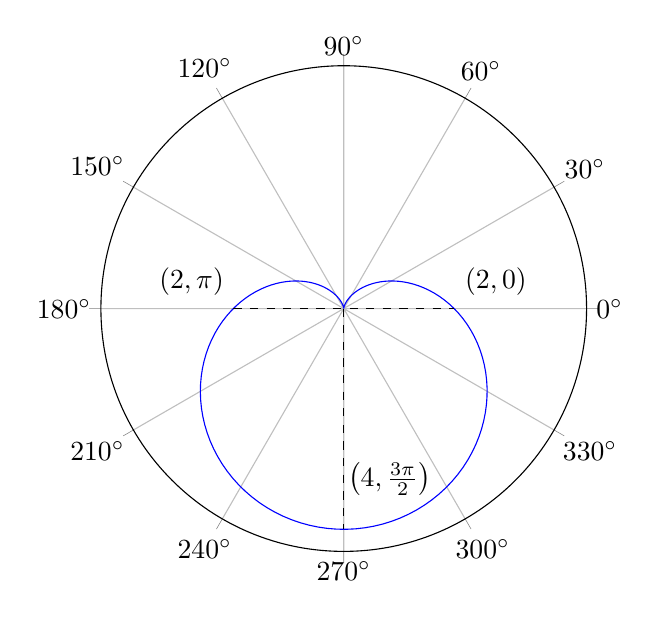
\begin{tikzpicture}
  \begin{polaraxis}[ytick=\empty, axis y line=none, xticklabel=$\pgfmathprintnumber{\tick}^\circ$, scale=0.9]
    \addplot [
      domain=0:2*pi,
      samples=150,
      blue,
      data cs=polarrad,
    ] {2-2*sin(deg(x))};

    \draw[dashed] (axis cs: 0,-2) -- (axis cs: 0,2);
    \node at (axis cs: -10,-2.8) {$(2,\pi)$};
    \node at (axis cs: 10,2.8) {$(2,0)$};
    \node at (axis cs: 285,3.2) {$\left(4,\frac{3\pi}2\right)$};
    \draw[dashed] (axis cs: 0,0) -- (axis cs: 270,4);

  \end{polaraxis}
\end{tikzpicture}
\end{center}

\noindent (b)
\begin{align*}A&=\frac12\int_a^br^2\,d\theta=\frac12\int_0^{2\pi}\left(2-2\sin\theta\right)^2\,d\theta=\frac12\int_0^{2\pi}\left(4-8\sin\theta+4\sin^2\theta\right)\,d\theta\\\\&=\frac12\int_0^{2\pi}\left(4-8\sin\theta+4\sin^2\theta\right)\,d\theta=\int_0^{2\pi}\left(2-4\sin\theta+1-\cos2\theta\right)\,d\theta\\\\&=\left[2\theta+4\cos\theta+\theta-\frac12\sin2\theta\right]_0^{2\pi}=\left[\left(4\pi+4+2\pi\right)-(4)\right]=\boxed{6\pi}\end{align*}

\hfill

\noindent (c) The slope of the tangent line in terms of $r$ and $\theta$ is

\[\left.\frac{dy}{dx}\right|_{(r,\theta)}=\frac{f'(\theta)\cdot\sin\theta+f(\theta)\cdot\cos\theta}{f'(\theta)\cdot\cos\theta-f(\theta)\cdot\sin\theta}\]

\[f(\theta)=2-2\sin\theta, \quad f'(\theta)=-2\cos\theta\]

\[\frac{dy}{dx}=\frac{-2\cos\theta\cdot\sin\theta+(2-2\sin\theta)\cdot\cos\theta}{-2\cos\theta\cdot\cos\theta-(2-2\sin\theta)\cdot\sin\theta}=\frac{-2\sin2\theta+2\cos\theta}{-\sin2\theta-2\sin\theta+2\sin^2\theta}\]

\[\left.\frac{dy}{dx}\right|_{\left(2-\sqrt2,\:\pi/4\right)}=\frac{-2+\sqrt2}{-\sqrt2}=\sqrt2-1\]

\hfill

\noindent The tangent vectors to the curve at $\theta=\dfrac\pi4$ are

\[\boxed{\left\langle k,\:k\left(\sqrt2-1\right)\right\rangle,\quad k\in\mathbb{R}}\]

\hfill

\noindent 2. 

\hfill

\noindent (a) Choose three arbitrary points and determine the parallel vector of each of the two line segments that connect the points.

\[\overrightarrow{AB}=\left\langle-1-0,\:0-(-1),\:1-1\right\rangle=\left\langle-1,1,0\right\rangle\]
\[\overrightarrow{AC}=\left\langle1-0,\:0-(-1),\:2-1\right\rangle=\left\langle1,1,1\right\rangle\]

\hfill

\noindent The cross product of these vectors gives us the normal vector of the plane.

\begin{align*}\mathbf{n}&=\left|\begin{array}{ccc}
\mathbf{i}&\mathbf{j}&\mathbf{k}\\
-1&1&0\\
1&1&1
\end{array}\right|=\mathbf{i}\left|\begin{array}{cc}
1&0\\1&1
\end{array}\right|-\mathbf{j}\left|\begin{array}{cc}
-1&0\\1&1
\end{array}\right|+\mathbf{k}\left|\begin{array}{cc}
-1&1\\1&1
\end{array}\right|\\\\&=(1\cdot1-0\cdot1)\mathbf{i}-(-1\cdot1-0\cdot1)\mathbf{j}+(-1\cdot1-1\cdot1)\mathbf{k}=\mathbf i+\mathbf j-2\mathbf k\end{align*}

\hfill

\noindent The plane has the equation $\mathbf n\cdot\overrightarrow{PP_0}=0$. Since $C(1,0,2)$ is on the plane, the equation of the plane is

\[\boxed{1(x-1)+1(y-0)-2(z-2)=0\implies x+y-2z+3=0}\]

\hfill

\noindent (b) Let $P$ be a point on a plane, then the distance from any point $R$ to the plane is the length of the vector projection of $\overrightarrow{PR}$ onto $\mathbf n$. That is,

\[d=\left|\overrightarrow{PR}\cdot\frac{\mathbf n}{|\mathbf n|}\right|\]

\hfill

\noindent The distance from $D$ to the plane passing through $A, B, C$ can be calculated using

\[d=\left|\overrightarrow{AD}\cdot\frac{\mathbf n}{|\mathbf n|}\right|=\left|\left\langle0-0,0-(-1),1-1\right\rangle\cdot\frac{\left\langle1,1,-2\right\rangle}{\sqrt{1^2+1^2+(-2)^2}}\right|=\boxed{\frac1{\sqrt6}}\]

\noindent (c) We have

\[\mathbf{v}=\overrightarrow{BD}=\left\langle0-(-1),0-0,1-1\right\rangle=\left\langle1,0,0\right\rangle\]

\hfill

\noindent The parametric equations for a line that passes through the point $P_0(x_0,y_0,z_0)$ is given by
\[\left.\begin{array}{c}
x=x_0+v_1t\\
y=y_0+v_2t\\
z=z_0+v_3t
\end{array}\right\}\quad t\in\mathbb{R}\]

\hfill

\noindent Therefore, the parametric equations for the line passing through $B$ and $D$ is

\[\boxed{\left.\begin{array}{l}
x=-1+t\\
y=0\\
z=1
\end{array}\right\}\quad t\in\mathbb{R}}\]

\hfill 

\noindent 3.

\hfill

\noindent (a)
\begin{center}
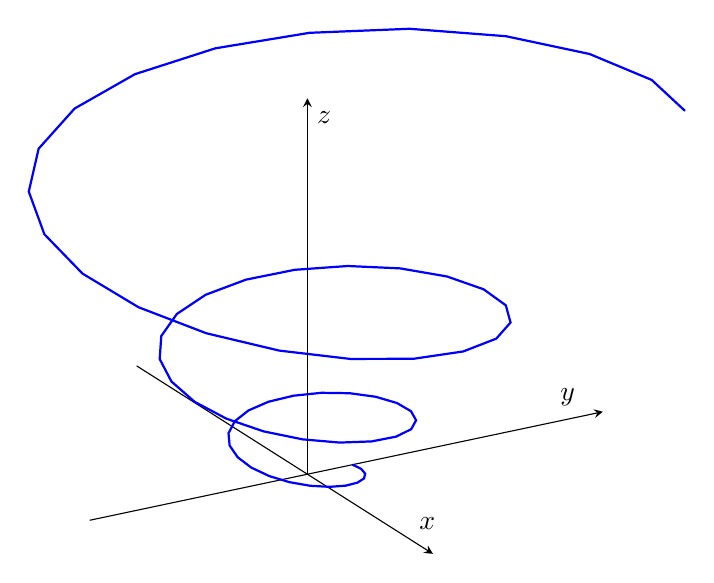
\begin{tikzpicture}
  \begin{axis}[
    view={60}{30},
    axis lines=center,
    xlabel={$x$}, ylabel={$y$}, zlabel={$z$},
    domain=0:2,
    samples=67,
    variable=t,
    xtick=\empty, ytick=\empty, ztick=\empty,
    restrict z to domain=0:7,
    scale=1.5,
  ]
    \addplot3[thick, blue] (
      {exp(t)*sin(deg(10*t))},
      {exp(t)*cos(deg(10*t))},
      {exp(t)}
    );
  \end{axis}
\end{tikzpicture}
\end{center}

\hfill

\noindent (b) The length of the parametrized curve $\mathbf{r}(t)=\left\langle x(t),\,y(t),\,z(t)\right\rangle$ for $a<t<b$ can be evaluated using the integral

\[L=\int_a^b\left|\frac{d\mathbf r}{dt}\right|\,dt\]

\hfill

\noindent The length of the curve is then

\begin{align*}L&=\int_0^1\left|\frac{d\mathbf r}{dt}\right|\,dt=\int_0^1\left|\left\langle\mathrm{e}^t\sin t+\mathrm{e}^t\cdot\cos t,\:\mathrm{e}^t\cos t-\mathrm{e}^t\sin t,\:\mathrm{e}^t\right\rangle\right|\,dt\\\\&=\int_0^1\sqrt{\left(\mathrm{e}^t\sin t+\mathrm{e}^t\cdot\cos t\right)^2+\left(\mathrm{e}^t\cos t-\mathrm{e}^t\sin t\right)^2+\left(\mathrm{e}^t\right)^2}\,dt\\\\&=\int_0^1\sqrt{\mathrm{e}^{2t}\left(\sin^2t+2\sin t\cos t+\cos^2t\right)+\mathrm{e}^t\left(\cos^2t-2\sin t\cos t+\sin^2t\right)+\mathrm{e}^{2t}}\,dt\\\\&=\int_0^1\sqrt{3\mathrm{e}^{2t}}\,dt=\int_0^1\sqrt3\mathrm e^t\,dt=\sqrt3\mathrm{e}^t\bigg|_0^1=\boxed{\sqrt3(\mathrm e-1)}\end{align*}

\hfill

\noindent 4.

\hfill

\noindent (a) Factor the denominator.

\begin{align*}\lim_{(x,y)\to(-1,-2)}\frac{y+2}{x^2y-xy+2x^2-2x}&=\lim_{(x,y)\to(-1,-2)}\frac{y+2}{x^2(y+2)-x(y+2)}\\\\&=\lim_{(x,y)\to(-1,-2)}\frac1{x^2-x}=\frac1{1-(-1)}=\boxed{\frac12}\end{align*}

\hfill

\noindent (b) Apply the Two-Path Test.

\[y=x\implies\lim_{(x,y)\to(0,0)}\frac{4x^2y}{x^4+y^2}=\lim_{(x,y)\to(0,0)}\frac{4x^3}{x^4+x^2}=\lim_{x\to0}\frac{4x}{x^2+1}=\frac01=0\]
\[y=x^2\implies\lim_{(x,y)\to(0,0)}\frac{4x^2y}{x^4+y^2}=\lim_{x\to0}\frac{4x^4}{2x^4}=\lim_{x\to0}\frac42=2\]

\hfill

\noindent Since $0\neq2$, by the Two-Path Test, the limit does not exist.

\hfill

\noindent 5.

\hfill

\noindent (a) Compute the first partial derivatives.

\[f_x=\frac1{x^2+y^2}\cdot2x=\frac{2x}{x^2+y^2},\qquad f_y=\frac1{x^2+y^2}\cdot2y=\frac{2y}{x^2+y^2}\]

\hfill

\noindent Compute the second partial derivatives.

\[f_{xx}=\frac{2\left(x^2+y^2\right)-(2x)\cdot(2x)}{\left(x^2+y^2\right)^2}=\frac{2y^2-2x^2}{\left(x^2+y^2\right)^2},\: f_{yy}=\frac{2\left(x^2+y^2\right)-(2y)\cdot(2y)}{\left(x^2+y^2\right)^2}=\frac{2x^2-2y^2}{\left(x^2+y^2\right)^2}\]
\[f_{xx}+f_{yy}=\frac{2y^2-2x^2}{\left(x^2+y^2\right)^2}+\frac{2x^2-2y^2}{\left(x^2+y^2\right)^2}=\boxed0\]

\hfill

\noindent (b)
\begin{center}
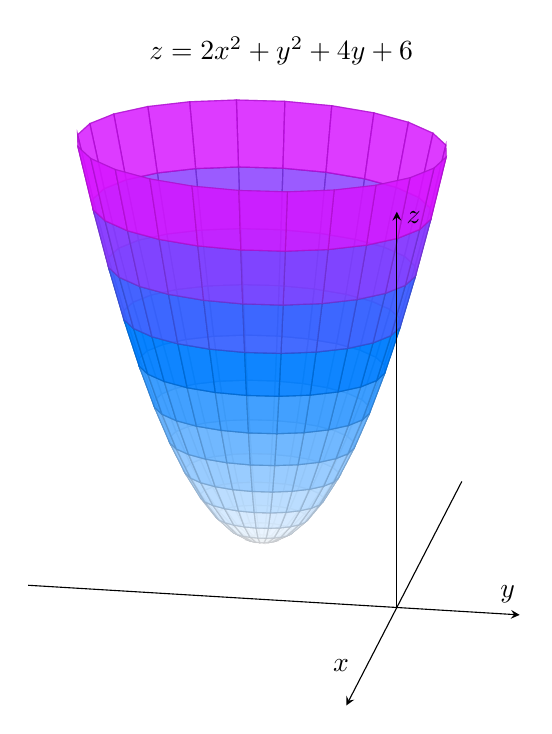
\begin{tikzpicture}
  \begin{axis}[
    title={$z=2x^2+y^2+4y+6$},
    title style={yshift=-10pt},
      view={100}{20},
      axis lines=center,
      axis equal image,
      xlabel={$x$},
      ylabel={$y$},
      zlabel={$z$},
      domain=0:2*pi,
      y domain=-2.25:2.25,
      samples=25,
      samples y=25,
      colormap/cool,
      axis on top,
      scale=1.5,
      xtick=\empty, ytick=\empty, ztick=\empty,
      z buffer=sort,
      xmin=-4.5, xmax=3.5,
      ymin=-4.5, ymax=1.5,
    ]
    \addplot3[
      surf,
      opacity=0.6
    ]
    ( {-2+(1/sqrt(2))*y*cos(deg(x))},
      {y*sin(deg(x))-2},
      {y^2} );
  \end{axis}
\end{tikzpicture}
\end{center}

\newpage


\begin{center}
2019-2020 Spring Midterm (08/06/2020) Solutions\\
(Last update: 28/08/2025 16:57)
\end{center}

\noindent 1. Let $M$ be the line $\dfrac{x-2}{-1}=\dfrac{y-1}{-2}=\dfrac{z-5}{1}=\lambda,\quad\lambda\in\mathbb{R}$. The direction vector of $M$ is $\mathbf u=\left\langle-1,-2,1\right\rangle$.

\hfill

\noindent Let $\mathbf v=\left\langle a,b,c\right\rangle$, where $a,b,c\in\mathbb R$, be the direction vector of $L$. If $M$ and $L$ are orthogonal, the dot product of the direction vectors is zero.

\[\mathbf u\cdot\mathbf v=\left\langle1,-2,1\right\rangle\cdot\left\langle a,b,c\right\rangle=a-2b+c=0\]

\hfill

\noindent $a,b,c$ could be any number with the relation $a-2b+c=0$. Let $a=1,\, b=1$. Then $c=2b-a=2-1=1$. The direction vector $\mathbf v$ is then $\mathbf v=\left\langle1,1,3\right\rangle$.

\hfill

\noindent The parametric equations for a line that passes through the point $P_0(x_0,y_0,z_0)$ is given by
\[\left.\begin{array}{c}
x=x_0+v_1t\\
y=y_0+v_2t\\
z=z_0+v_3t
\end{array}\right\}\quad t\in\mathbb{R}\]

\hfill

\noindent Therefore, using the point $P$, the parametric equations for the line $L$ is

\[\boxed{\left.\begin{array}{l}
x=-1+t\\
y=3+t\\
z=1+3t
\end{array}\right\}\quad t\in\mathbb{R}}\]

\hfill

\noindent 2.

\hfill

\noindent (a)
\begin{center}
    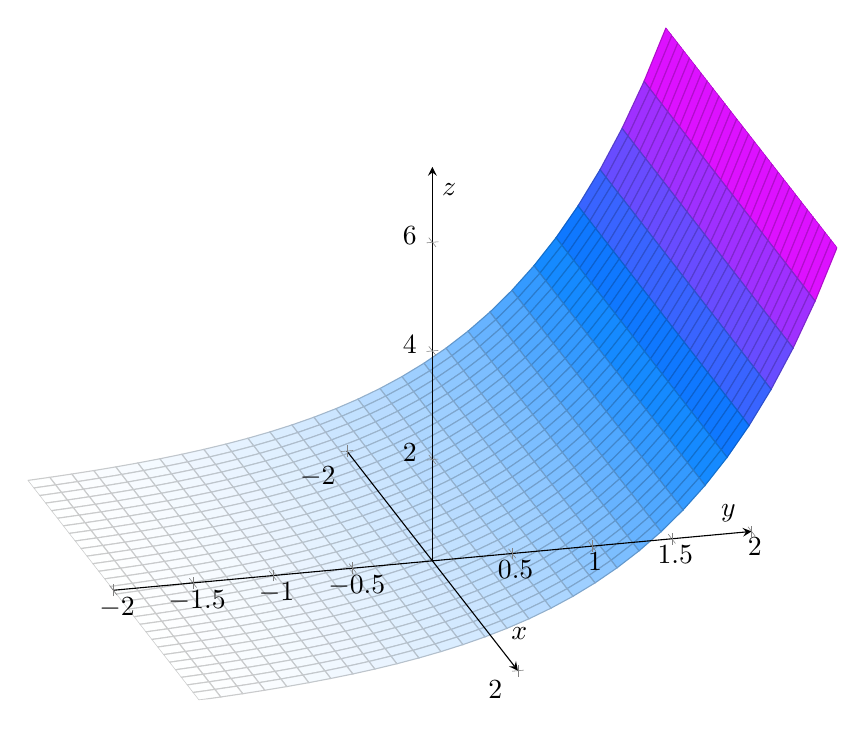
\begin{tikzpicture}
  \begin{axis}[
    view={75}{30},
    axis lines=center,
    xlabel={$x$},
    ylabel={$y$},
    zlabel={$z$},
    domain=-2:2,
    samples=30,
    colormap/cool,
    mesh/ordering=y varies,
    scale=1.5,
    axis on top,
  ]
    \addplot3[surf]  (x, y, {e^y});
  \end{axis}
\end{tikzpicture}
\end{center}

\newpage

\noindent (b)
\begin{center}
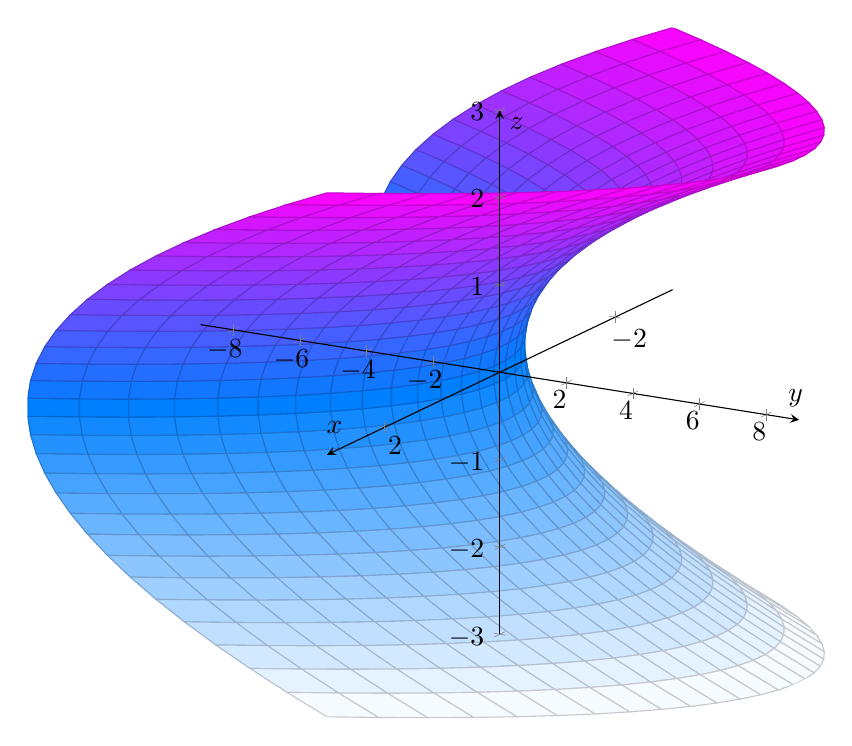
\begin{tikzpicture}
  \begin{axis}[
    view={120}{20},
    axis lines=center,
    xlabel={$x$},
    ylabel={$y$},
    zlabel={$z$},
    domain=-3:3,
    y domain=-3:3,
    samples=30,
    samples y=30,
    colormap/cool,
    z buffer=sort,
    axis on top,
    scale=1.75
  ]
    \addplot3[surf]({x}, {y^2 - x^2}, {y});
  \end{axis}
\end{tikzpicture}
\end{center}

\hfill

\noindent 3. The velocity and acceleration vectors can be obtained by taking the first and the second derivatives of the vector function with respect to the parametrization variable, respectively.

\[\text{Velocity vector}:\mathbf v(t)=\frac{d\mathbf R}{dt}=\left\langle-2\sin t,\,2t,\,2\cos t\right\rangle\]

\[\text{Acceleration vector}:\mathbf a(t)=\frac{d\mathbf v}{dt}=\left\langle-2\cos t,\,2,\,-2\sin t\right\rangle\]

\hfill

\noindent The speed of motion is the magnitude of the velocity vector, and the direction is the normalized velocity vector.

\[\text{Speed}=\left|\mathbf v(t=\pi/2)\right|=\sqrt{\left(-2\sin\frac\pi2\right)^2+\left(2\cdot\frac\pi2\right)^2+\left(2\cos\frac\pi2\right)^2}=\sqrt{4+\pi^2}\]

\[\text{Direction}=\frac{\mathbf v(t=\pi/2)}{\left|\mathbf v(t=\pi/2)\right|}=\frac{\left\langle-2\sin\dfrac\pi2,\,2\cdot\dfrac\pi2,\,2\cos\dfrac\pi2\right\rangle}{\sqrt{4+\pi^2}}=\left\langle-\frac2{\sqrt{4+\pi^2}},\,\frac\pi{\sqrt{4+\pi^2}},0\right\rangle\]

\hfill

\[\boxed{\begin{array}{c}
\mathbf v(t)=\left\langle-2\sin t,\,2t,\,2\cos t\right\rangle\\
\mathbf a(t)=\left\langle-2\cos t,\,2,\,-2\sin t\right\rangle\\[1em]
\text{Speed of motion at }t=\dfrac\pi2:\sqrt{4+\pi^2}\\
\text{Direction of motion at }t=\dfrac\pi2:\left\langle-\dfrac2{\sqrt{4+\pi^2}},\,\dfrac\pi{\sqrt{4+\pi^2}},0\right\rangle\\
\end{array}}\]

\newpage

\noindent 4. Apply the Two-Path Test.

\[x=y\implies\lim_{(x,y)\to(0,0)}\frac{xy^3}{x^2+y^6}=\lim_{y\to0}\frac{y^4}{y^2+y^6}=\lim_{y\to0}\frac{y^2}{1+y^4}=\frac01=0\]
\[x=y^3\implies\lim_{(x,y)\to(0,0)}\frac{xy^3}{x^2+y^6}=\lim_{y\to0}\frac{y^6}{y^6+y^6}=\lim_{y\to0}\frac{y^6}{2y^6}=\frac12\]

\hfill

\noindent Since $0\neq\dfrac12$, by the Two-Path Test, the limit does not exist. Therefore, the function $f$ is not continuous at $(0,0)$.

\hfill

\noindent 5. The value of the function at the point $(0,0)$ is $0$. Therefore, we will show that the limit $L$ is also $0$. For every $\epsilon>0$, there exists a $\delta>0$ such that

\[0<\sqrt{(x-0)^2+(y-0)^2}<\delta\implies\left|f(x,y)-L\right|<\epsilon\]

\begin{align*}\left|\frac{x^2y}{x^2+y^6}-0\right|&=|y|\cdot\left|\frac{x^2}{x^2+y^6}\right|\leq|y|\cdot1=|y|\qquad\left[\frac{x^2}{x^2+y^6}\leq\frac{x^2}{x^2}=1\right]\\\\&\leq|x|+|y|<2\delta\qquad\left[x^2\geq0,\,y^2\geq0,\,\sqrt{x^2+y^2}<\delta\implies|x|<\delta,\,|y|<\delta\right]\end{align*}

\hfill

\noindent Let $\delta=\dfrac\epsilon2$.

\[\left|\frac{x^2y}{x^2+y^6}\right|\leq|x|+|y|=2\cdot\frac\epsilon2=\epsilon\]

\hfill

\noindent Since the limit is equal to the value of the function at $(0,0)$, $f$ is continuous at $(0,0)$.

\hfill

\noindent 6. $u$ and $v$ are functions of $x$ and $y$. $x$ and $y$ are functions of $r$ and $\theta$. Use the chain rule.

\[\frac{\partial u}{\partial r}=\frac{\partial u}{\partial x}\cdot\frac{\partial x}{\partial r}+\frac{\partial u}{\partial y}\cdot\frac{\partial y}{\partial r}=u_x\cdot\cos\theta+u_y\cdot\sin\theta=v_y\cos\theta-v_x\sin\theta\]

\[\frac{\partial v}{\partial\theta}=\frac{\partial v}{\partial x}\cdot\frac{\partial x}{\partial\theta}+\frac{\partial v}{\partial y}\cdot\frac{\partial y}{\partial\theta}\implies\frac1r\frac{\partial v}{\partial\theta}=\frac1r\left(-v_x\cdot r\sin\theta+v_y\cdot r\cos\theta\right)=-v_x\sin\theta+v_y\cos\theta\]

\[\frac{\partial u}{\partial r}=-v_x\sin\theta+v_y\cos\theta=\frac1r\frac{\partial v}{\partial\theta}\]

\hfill

\[\frac{\partial v}{\partial r}=\frac{\partial v}{\partial x}\cdot\frac{\partial x}{\partial r}+\frac{\partial v}{\partial y}\cdot\frac{\partial y}{\partial r}=v_x\cdot\cos\theta+v_y\cdot\sin\theta=-u_y\cos\theta+u_x\sin\theta\]

\[\frac{\partial u}{\partial\theta}=\frac{\partial u}{\partial x}\cdot\frac{\partial x}{\partial\theta}+\frac{\partial u}{\partial y}\cdot\frac{\partial y}{\partial\theta}\implies-\frac1r\frac{\partial u}{\partial\theta}=-\frac1r\left(-u_x r\sin\theta+u_y r\cos\theta\right)=u_x\sin\theta-u_y\cos\theta\]

\[\frac{\partial v}{\partial r}=u_x\sin\theta-u_y\cos\theta=-\frac1r\frac{\partial u}{\partial \theta}\]

\hfill

\noindent 7. The total differential of $R$ is

\[dR=\frac{\partial R}{\partial x}\,dx+\frac{\partial R}{\partial r}\,dr=\frac c{r^4}\,dx-\frac{4cx}{r^5}\,dr\]

\hfill

\noindent Since we estimate the percent change in $R$, we may take $\Delta R\approx dR$. Therefore, $dx=x\cdot3\%,\,dr=r\cdot(-2\%)$. Given also $x=8\,\text{cm},\,r=2\, \text{mm}=0.2\,\text{cm}$, the percent change can be estimated as

\[\frac{dR}R\cdot100\%=\frac1{\frac{cx}{r^4}}\cdot\left(\frac c{r^4}\cdot x\cdot3\%-\frac{4cx}{r^5}\cdot r\cdot(-2\%)\right)\cdot100\%=\boxed{11\%}\]

\hfill

\noindent 8. To identify the critical points, find where both $f_x=f_y=0$ or one of the partial derivatives does not exist.

\[f_x=-3x^2+9,\quad f_y=-8y\]
\[\left.\begin{array}{c}
f_x=0\implies9=3x^2\\
f_y=0\implies-8y=0 
\end{array}\:\right\}\quad y=0,\:x=\pm\sqrt3\]

\hfill

\noindent The critical points are $\left(\sqrt3,0\right)$ and $\left(-\sqrt3,0\right)$. To classify these points, calculate the second partial derivatives and then find the Hessian determinants.

\[f_{xx}=-6x,\quad f_{xy}=f_{yx}=0,\quad f_{yy}=-8\]

\[\left(\sqrt3,0\right)\rightarrow\left\{\:\begin{array}{l}
f_{xx}=-6\sqrt3,\quad f_{xy}=0,\quad f_{yy}=-8\\[1em]
\left|\begin{array}{cc}
-6\sqrt3 & 0\\
0 & -8
\end{array}\right|=\left(-6\sqrt3\right)\cdot(-8)-0\cdot0=48\sqrt3>0,\quad f_{xx}<0
\end{array}\right.\]

\[\left(-\sqrt3,0\right)\rightarrow\left\{\:\begin{array}{l}
f_{xx}=6\sqrt3,\quad f_{xy}=0,\quad f_{yy}=-8\\[1em]
\left|\begin{array}{cc}
6\sqrt3 & 0\\
0 & -8
\end{array}\right|=\left(-6\sqrt3\right)\cdot(-8)-0\cdot0=-48\sqrt3<0
\end{array}\right.\]

\[\boxed{\text{A local maximum occurs at }\left(\sqrt3,0\right)\text{ and a saddle point occurs at }\left(-\sqrt3,0\right).}\]

\newpage


\begin{center}
2019-2020 Summer Midterm (15/08/2020) Solutions\\
(Last update: 30/08/2025 01:52)
\end{center}

\noindent 1. The normal vector of the plane is the gradient vector. Find the normal vectors of the planes and calculate the cross product of these vectors. The resulting vector is parallel to the intersection of the planes.
\[\mathbf{n}_1=\left\langle1,-1,0\right\rangle,\qquad \mathbf{n}_2=\left\langle3,0,1\right\rangle\]
\[\mathbf{v}=\mathbf{n}_1\times\mathbf{n}_2=\left|\begin{array}{ccc}
\mathbf{i}&\mathbf{j}&\mathbf{k}\\
1&-1&0\\
3&0&1
\end{array}\right|=\mathbf{i}\left|\begin{array}{cc}
-1&0\\0&1
\end{array}\right|-\mathbf{j}\left|\begin{array}{cc}
1&0\\3&1
\end{array}\right|+\mathbf{k}\left|\begin{array}{cc}
1&-1\\3&0
\end{array}\right|=-\mathbf{i}-\mathbf{j}+3\mathbf{k}\]

\hfill

\noindent The parametric equations for a line that passes through the point $P_0(x_0,y_0,z_0)$ is given by
\[\left.\begin{array}{c}
x=x_0+v_1t\\
y=y_0+v_2t\\
z=z_0+v_3t
\end{array}\right\}\quad t\in\mathbb{R}\]

\hfill

\noindent Therefore, the parametric equations for the line $L$ is

\[\boxed{\left.\begin{array}{l}
x=-t\\
y=2-t\\
z=1+3t
\end{array}\right\}\quad t\in\mathbb{R}}\]

\hfill

\noindent 2. The vector that is parallel to the direction of the line is
\[\mathbf u=\left\langle-1-1,0-2,4-1\right\rangle=\left\langle-2,-2,3\right\rangle\]

\noindent If the vectors $\mathbf v$ and $\mathbf u$ are orthogonal, the dot product of these two vectors must be equal to zero.
\[\mathbf v\times \mathbf u=\left\langle1,5,4\right\rangle\cdot\left\langle-2,-2,3\right\rangle=1\cdot(-2)+5\cdot(-2)+4\cdot3=-2-10+12=0\]

\noindent 3.

\hfill

\noindent (a)
\begin{center}
    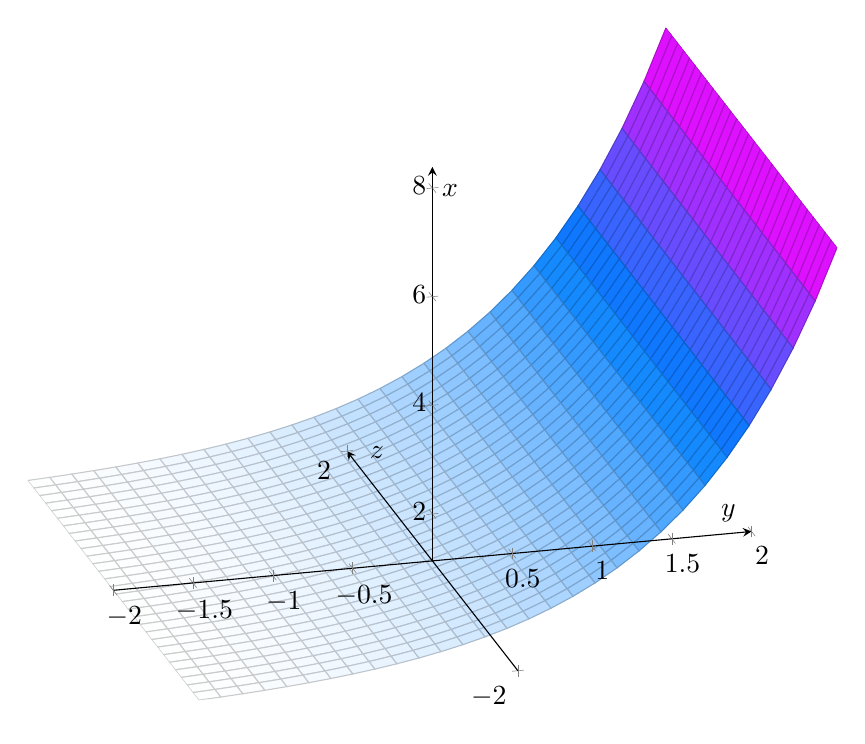
\begin{tikzpicture}
  \begin{axis}[
    view={-15}{30},
    axis lines=center,
    xlabel={$y$},
    ylabel={$z$},
    zlabel={$x$},
    domain=-2:2,
    samples=30,
    colormap/cool,
    mesh/ordering=y varies,
    scale=1.5,
    axis on top,
  ]
    \addplot3[surf]{exp(x)+1};
  \end{axis}
\end{tikzpicture}
\end{center}

\hfill

\noindent (b)
\begin{center}
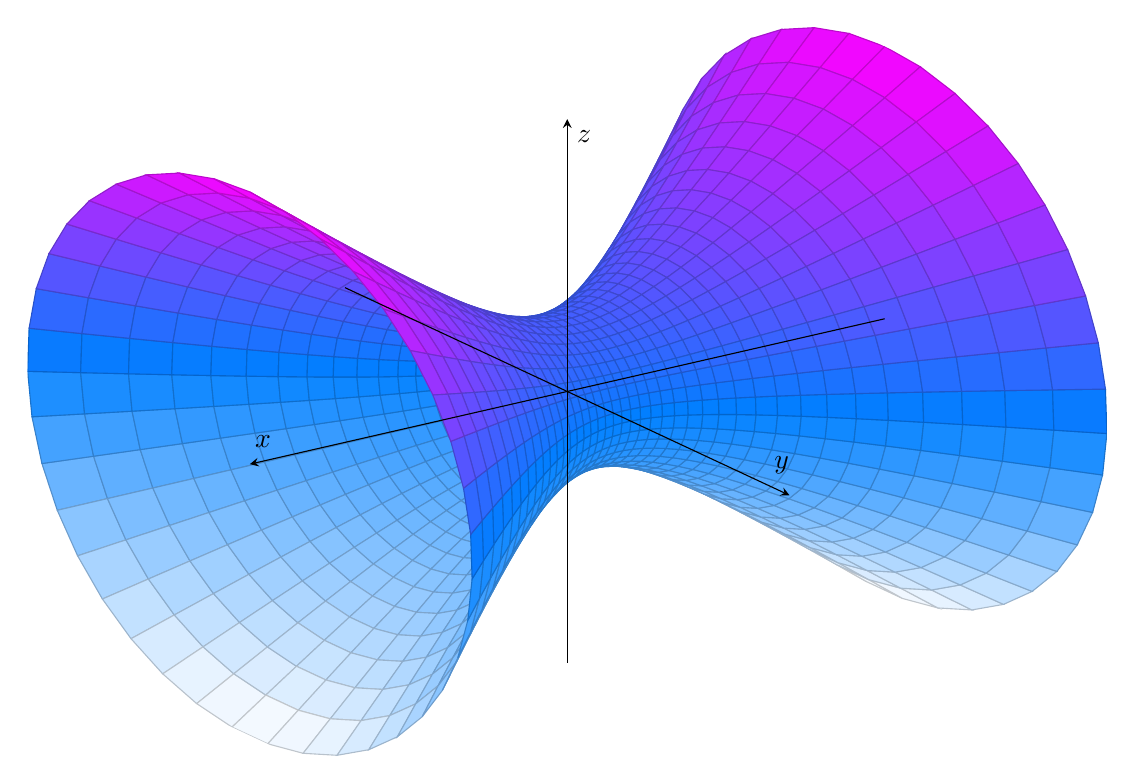
\begin{tikzpicture}
  \begin{axis}[
    view={145}{25},
    xlabel={$x$},
    ylabel={$y$},
    zlabel={$z$},
    axis lines=center,
    domain=0:360,
    y domain=-2:2,
    samples=40,
    axis on top,
    colormap/cool,
    scale=2,
    ticklabel style={anchor=base},
    z buffer=sort, 
    xtick=\empty, ytick=\empty, ztick=\empty,
  ]
  
  \addplot3[surf] ({sinh(y)},{cosh(y)*sin(x)},{cosh(y)*cos(x)});
  \end{axis}
\end{tikzpicture}
\end{center}

\hfill

\noindent 4. Apply the Two Different Paths Test.

\[y=x\implies\lim_{(x,y)\to(0,0)}\frac{x^5y^3}{x^7+y^{21/2}}=\lim_{x\to0}\frac{x^8}{x^7\left(1+x^{7/2}\right)}=\lim_{x\to0}\frac x{1+x^{7/2}}=\frac01=0\]
\[y=x^{2/3}\implies\lim_{(x,y)\to(0,0)}\frac{x^5y^3}{x^7+y^{21/2}}=\lim_{x\to0}\frac{x^7}{2x^7}=\frac12\]

\hfill

\noindent Since $0\neq\dfrac12$, by the Two Different Paths Test, the limit does not exist.

\hfill

\noindent 5. For every $\epsilon>0$, there exists a $\delta>0$ such that

\[0<\sqrt{(x-0)^2+(y-0)^2}<\delta\implies\left|f(x,y)-L\right|<\epsilon\]

\hfill

\noindent The value of the function at $(0,0)$ is $f(0,0)=6\cdot0^2+7\cdot0^2=0$. So, we expect that the limit of the function at this point is $0$.

\[\left|6x^2+7y^2\right|=6x^2+7y^2\qquad\left[x^2\geq0,\quad y^2\geq0\right]\]
\[6x^2+7y^2\leq7x^2+7y^2=7\left(x^2+y^2\right)<7\delta^2\qquad\left[0<\sqrt{x^2+y^2}<\delta\right]\]

\hfill

\noindent Set $\delta=\sqrt{\dfrac\epsilon7}$.

\[\left|f(x,y)-L\right|=|6x^2+7y^2-0|=6x^2+7y^2<7\delta^2=\epsilon\]

\hfill

\noindent Since the limit is the value of the function at this point, $f$ is continuous at $(x,y)=(0,0)$.

\hfill

\noindent 6. $w$ is a function of $x,\:y,\:z$ and $x,\:y,\:z$ are functions of $r,\:s,\:t$. Namely, $w=w(x,y,z),\:x=x(r,s,t),\:y=y(r,s,t),\:z=z(r,s,t)$. Apply the chain rule.

\[\frac{\partial w}{\partial r}=\frac{\partial w}{\partial x}\cdot\frac{\partial x}{\partial r}+\frac{\partial w}{\partial y}\cdot\frac{\partial y}{\partial r}+\frac{\partial w}{\partial z}\cdot\frac{\partial z}{\partial r}\]

\[\frac{\partial w}{\partial x}=\mathrm{e}^{2x-y+3z^2}\cdot2,\quad\frac{\partial w}{\partial y}=\mathrm{e}^{2x-y+3z^2}\cdot(-1),\quad\frac{\partial w}{\partial z}=\mathrm{e}^{2x-y+3z^2}\cdot(6z)\]

\[\frac{\partial x}{\partial r}=1,\quad\frac{\partial y}{\partial r}=2,\quad\frac{\partial z}{\partial r}=-2\sin(rst)\cdot st\]

\[\frac{\partial w}{\partial r}=2\mathrm{e}^{2x-y+3z^2}-2\mathrm{e}^{2x-y+3z^2}-12z\mathrm{e}^{2x-y+3z^2}\sin(rst)st=\boxed{-12zst\cdot\mathrm{e}^{2x-y+3z^2}\cdot\sin(rst)}\]

\hfill

\noindent 7. The volume and the surface area of a right circular cylinder are as follows, respectively.

\[V(D,h)=\frac{\pi D^2h}4,\quad S(D,h)=\pi Dh+\frac{\pi D^2}2,\]

\noindent where $D$ is the diameter of the base and $D=2r$.

\hfill

\noindent (a) The total differential of $V$ is

\[dV=V_D\cdot dD+V_h\cdot dh\]

\hfill

\noindent Calculate the partial derivatives.

\[V_D=\frac{\pi Dh}2,\quad V_h=\frac{\pi D^2}4\]

\hfill

\noindent It is given $\left|dD\right|\leq0.5,\:|dh|\leq0.5,\:D=4,\:h=8$. The bounds for the propagated error in calculating the volume is

\[|dV|\leq\frac{\pi\cdot4\cdot8}2\cdot0.5+\frac{\pi\cdot4^2}4\cdot0.5=8\pi+2\pi=\boxed{10\pi\:\text{cm}^3}\]

\hfill

\noindent (b) The total differential of $S$ is

\[dS=S_D\cdot dD+S_h\cdot dh\]

\hfill

\noindent Calculate the partial derivatives.

\[S_D=\pi h+\pi D,\quad S_h=\pi D\]

\hfill

\noindent It is given $\left|dD\right|\leq0.5,\:|dh|\leq0.5,\:D=4,\:h=8$. The bounds for the propagated error in calculating the surface area is

\[|dS|=\pi\left(8+4\right)\cdot0.5+4\pi\cdot0.5=6\pi+2\pi=\boxed{8\pi\:\text{cm}^2}\]

\hfill

\noindent 8. The normal vector to the surface is $\left\langle0,\ln z,\frac yz+1\right\rangle$. At the point $(1,0,2)$, the normal vector is $\left\langle0,\ln2,1\right\rangle$. The dot product of the normal vector to the surface and the vector that is parallel to the direction of the line is $0$. Let $\mathbf v=\langle 0,b,c\rangle$ be the direction vector of the line. The $x$-component is $0$ because the line is parallel to the $yz$-plane.

\[\langle0,\ln2,1\rangle\cdot\langle0,b,c\rangle=b\ln2+c=\implies \frac cb=-\ln2\]

\hfil

\noindent The slope of the line is $\dfrac{dz}{dy}$ on the $yz$-plane, which is $\dfrac cb$. Therefore, the slope is $\boxed{-\ln2}$.

\hfill

\noindent 9. The equation for the tangent plane to the surface defined by $z=f(x,y)$ at a point $P_0(x_0,y_0,z_0)$ is given by $z-z_0=f_x(x-x_0)+f_y(y-y_0)$.

\[x_0=0,\quad y_0=1,\quad z_0=3,\quad f_x=\cos x+y\mathrm{e}^{xy},\quad f_y=x\mathrm{e}^{xy}+2\]
\[P=(0,1,3)\quad\rightarrow\quad f_x(0,1)=2,\quad f_y(0,1)=2\]

\hfill

\noindent The equation for the tangent plane is

\[\boxed{z-3=2(x-0)+2(y-1)\implies z=2x+2y+1}\]

\newpage


\begin{center}
2020-2021 Spring Midterm (28/04/2021) Solutions\\
(Last update: 28/08/2025 14:04)
\end{center}

\noindent 1.

\hfill

\noindent (a) Two lines are skew if they do not intersect and are not parallel.

\hfill

\noindent Let $L$ be the line $x-1=\dfrac z3,\: y=0$  and $M$ be the line $\displaystyle x=\frac{y+1}2=z$. Let $\mathbf u$ and $\mathbf v$ be the vectors that are parallel to these lines, respectively. Using the coefficients from the symmetric equations, we have $\mathbf u=\langle1,0,3\rangle, \:\mathbf v= \langle1,2,1\rangle$. If the cross product of these vectors is a non-zero vector, they are not parallel.
\[\mathbf{n}=\mathbf{u}\times\mathbf{v}=\left|\begin{array}{ccc}
\mathbf{i}&\mathbf{j}&\mathbf{k}\\
1&0&3\\
1&2&1
\end{array}\right|=\mathbf{i}\left|\begin{array}{cc}
0&3\\2&1
\end{array}\right|-\mathbf{j}\left|\begin{array}{cc}
1&3\\1&1
\end{array}\right|+\mathbf{k}\left|\begin{array}{cc}
1&0\\1&2
\end{array}\right|=-6\mathbf{i}+2\mathbf{j}+2\mathbf{k}\neq\mathbf{0}\]

\hfill

\noindent Parametrize the lines and determine whether they intersect.

\[L=\left\{\begin{array}{l}
x=1+t\\
y=0\\
z=3t
\end{array}\right.\quad t\in\mathbb{R}\qquad\qquad M=\left\{\begin{array}{l}
x=s\\
y=2s-1\\
z=s
\end{array}\right.\quad s\in\mathbb{R}\]

\hfill

\noindent Compare the $y$-components. If $2s-1=0$, then $s=\dfrac12$. If we substitute the value for $s$ in the $x$- and $z$- components and compare, we obtain $1+t=\dfrac12$ and $3t=\dfrac12$.

\[1+t=\frac12\implies t=\frac12,\qquad 3t=\frac12\implies t=\frac32\]
\[\frac12\neq\frac32\]

\hfill

\noindent This leads to a contradiction that the lines intersect. Since the lines do not intersect and are not parallel, the lines are skew.

\hfill

\noindent (b) From (a), we have the normal vector $\mathbf n$ of the plane. The equation for the tangent plane with the normal vector $\mathbf n$ containing the point $P_0(x_0,y_0,z_0)$ is given by $n_1(x-x_0)+n_2(y-y_0)+n_3(z-z_0)=0$.

\[x_0=1,\quad y_0=3,\quad z=5,\quad \mathbf n=-6\mathbf{i}+2\mathbf{j}+2\mathbf{k}\]

\hfill

\noindent The equation for the tangent plane is

\[-6(x-1)+2(y-3)+2(z-5)=0\implies\boxed{-3x+y+z=5}\]

\newpage

\noindent 2.

\hfill

\noindent (a)
\begin{center}
    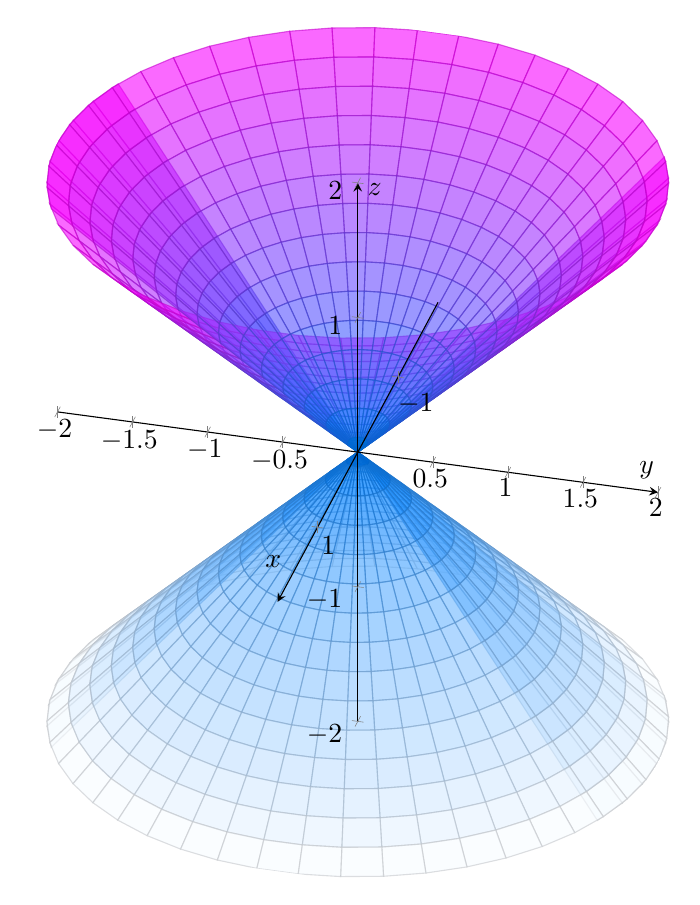
\begin{tikzpicture}
  \begin{axis}[
    view={105}{30},
    axis lines=center,
    axis equal image,
    xlabel={$x$},
    ylabel={$y$},
    zlabel={$z$},
    domain=-2:2,
    samples=30,
    colormap/cool,
    mesh/ordering=y varies,
    scale=3,
    axis on top,
  ]
  \addplot3 [surf,z buffer=sort,opacity=0.6] ({x*cos(deg(y))}, {x*sin(deg(y))}, {x});
  \addplot3 [surf,z buffer=sort,opacity=0.6] ({x*cos(deg(y))}, {x*sin(deg(y))}, {-x});
  \end{axis}
\end{tikzpicture}
\end{center}

\hfill

\noindent (b)
\begin{center}
    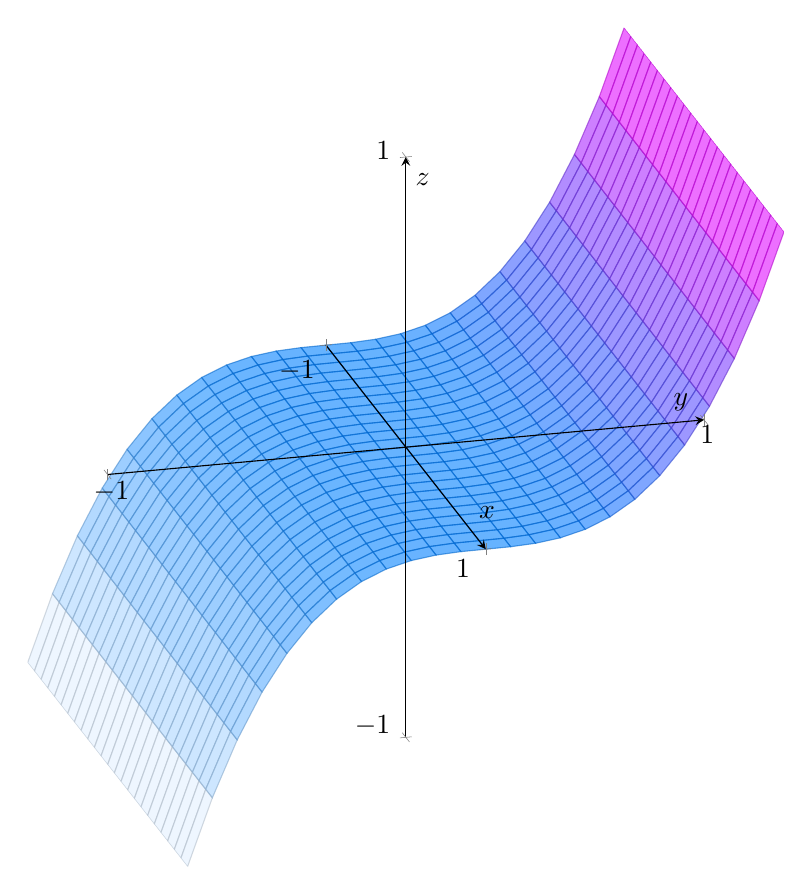
\begin{tikzpicture}
  \begin{axis}[
    view={75}{20},
    axis equal image,
    axis lines=center,
    xlabel={$x$},
    ylabel={$y$},
    zlabel={$z$},
    domain=-1:1,
    samples=25,
    colormap/cool,
    scale=2.2,
    axis on top,
    xtick={-1,1}, ytick={-1,1}, ztick={-1,1},
  ]
  \addplot3 [surf,z buffer=sort,opacity=0.6] {y^3};
  \end{axis}
\end{tikzpicture}
\end{center}

\newpage

\noindent 3. Find $\mathbf{R}(1)$.

\[\mathbf{R}(1)=\mathbf{i}-\mathbf{k}\]

\hfill

\noindent For $t=1$, we have the point $(1,0,-1)$ on the curve. The tangent vector of this curve is the first derivative of $\mathbf{R}$ with respect to the parametrization variable.

\begin{align*}\mathbf{T}=\frac{d\mathbf R}{dt}&=\left(\frac d{dt}\left(1+2\sin(2\pi t)\right)\right)\mathbf{i}+\left(\frac d{dt}\ln t\right)\mathbf{j}+\left(\frac d{dt}\cos(\pi t)\right)\mathbf{k}\\\\&=(4\pi\cos(2\pi t))\mathbf{i}+\left(\frac1t\right)\mathbf{j}+(-\pi\sin(\pi t))\mathbf{k}\end{align*}

\hfill

\noindent At $t=1$, the tangent vector is $\mathbf{T}(1)=\left(4\pi\right)\mathbf{i}+\mathbf{j}$. The parametric equations for a line that passes through the point $P_0(x_0,y_0,z_0)$ is given by
\[\left.\begin{array}{c}
x=x_0+T_1u\\
y=y_0+T_2u\\
z=z_0+T_3u
\end{array}\right\}\quad u\in\mathbb{R}\]

\hfill

\noindent Therefore, the equation of the line that is tangent to $C$ is

\[\boxed{\left.\begin{array}{l}
x=1+4\pi u\\
y=u\\
z=-1
\end{array}\right\}\quad u\in\mathbb{R}}\]

\hfill

\noindent 4. The value of the function at the point $(1,-2)$ is $4$. Therefore, we will show that the limit is also $4$. For every $\epsilon>0$, there exists a $\delta>0$ such that

\[0<\sqrt{(x-1)^2+(y+2)^2}<\delta\implies\left|f(x,y)-L\right|<\epsilon\]

\begin{align*}\left|\frac{4x^2-y}{2x+y}-4\right|&=\left|\frac{(2x-y)(2x+y)}{2x+y}-4\right|=\left|2x-y-4\right|=\left|2(x-1)+(-y-2)\right|\\\\&\leq2|x-1|+\left|-y-2\right|\quad \left(|a+b|\leq|a|+|b|\rightarrow\text{triangle inequality}\right)\\\\&=2|x-1|+|y+2|\end{align*}

\hfill

\noindent Since $\sqrt{(x-1)^2+(y+2)^2}<\delta\implies(x-1)^2+(y+2)^2<\delta^2$ and $(x-1)^2\geq0$ and $(y+2)^2\geq0$, we have $|x-1|\leq\delta$ and $|y+2|\leq\delta$.

\[2|x-1|+|y+2|\leq2\delta+\delta=3\delta\]

\hfill

\noindent Let $\delta=\dfrac\epsilon3$.

\[\left|\frac{4x^2-y}{2x+y}-4\right|\leq2|x-1|+|y+2|\leq3\cdot\frac\epsilon3=\epsilon\]

\hfill

\noindent Since the limit is equal to the value of the function at $(-1,2)$, $f$ is continuous at $(-1,2)$.

\hfill

\noindent 5. Apply the chain rule.

\[\frac{\partial w}{\partial u}=\frac{\partial w}{\partial x}\cdot\frac{\partial x}{\partial u}+\frac{\partial w}{\partial y}\cdot\frac{\partial y}{\partial u}+\frac{\partial w}{\partial z}\cdot\frac{\partial z}{\partial u}\]
\[\frac{\partial w}{\partial x}=\frac1z,\quad\frac{\partial w}{\partial y}=\frac{\cos y}z,\quad \frac{\partial w}{\partial z}=-\frac{x+\sin y}{z^2}\]
\[\frac{\partial x}{\partial u}=\frac1{u+v},\quad\frac{\partial y}{\partial u}=v\mathrm{e}^{uv},\quad\frac{\partial z}{\partial u}=-\frac1{u^2}\]

\begin{align*}\frac{\partial w}{\partial u}&=\frac1z\cdot\frac1{u+v}+\frac{\cos y}z\cdot v\mathrm{e}^{uv}+\frac{x+\sin y}{z^2}\cdot\frac1{u^2}\\\\&=\boxed{\frac u{u+v}+\mathrm{e}^{uv}uv\cos\left(\mathrm{e}^{uv}\right)+\ln(u+v)+\sin\left(\mathrm{e}^{uv}\right)}\end{align*}

\hfill

\noindent 6. The volume of a right triangular prism with opposite and adjacent sides and height $a=5,\:b=3,\:h=6$ is given by

\[V(a,b,h)=\frac12 abh\]

\hfill

\noindent For small errors, $\Delta V\approx dV$. The total differential of $V$ is

\[dV=V_ada+V_bdb+V_hdh\]

\hfill

\noindent Compute $V_a,\: V_b,\: V_c$.

\[V_a=\frac12bh=\frac12\cdot3\cdot6=9,\quad V_b=\frac12ah=\frac12\cdot5\cdot6=15,\quad V_h=\frac12ab=\frac12\cdot5\cdot3=\frac{15}2\]

\hfill

\noindent Given that $|da|\leq0.4,\:|db|\leq0.4,\:|dh|\leq0.4$. Calculate the bounds for the propagated error.

\[\left|dV\right|\leq9\cdot0.4+15\cdot0.4+\frac{15}2\cdot0.4=\boxed{\frac{63}5}\]

\hfill

\noindent 7. Let $g(x,y,z)=x^2+2y^2+z^2-1$ be the constraint. Solve the system of equations below.

\[
\left.
\begin{array}{c}
\displaystyle\nabla f=\lambda\nabla g\\
\displaystyle g(x,y,z)=0
\end{array}
\right\}\quad
\begin{array}{l}
\nabla f=\left\langle1,0,-1\right\rangle=\lambda\left\langle2x,4y,2z\right\rangle=\lambda\nabla g\\[1em]x=\dfrac1{2\lambda},\quad y=0\:\text{ or }\:\lambda=0,\quad z=-\dfrac1{2\lambda}
\end{array}
\]

\hfill

\[\lambda=0\implies x=y=z=0\implies f(0,0,0)=0\]

\[x=\frac1{2\lambda},\quad y=0,\quad z=-\frac1{2\lambda}\implies g\left(\frac1{2\lambda},0,-\frac1{2\lambda}\right)=\left(\frac1{2\lambda}\right)^2+2\cdot0^2+\left(-\frac1{2\lambda}\right)^2=1\]
\[\frac1{2\lambda^2}=1\implies\lambda=\pm\frac1{\sqrt2}\]

\hfill

\[\lambda=\frac1{\sqrt2}\implies x=\frac1{\sqrt2},\: y=0,\: z=-\frac1{\sqrt2}\qquad\lambda=-\frac1{\sqrt2}\implies x=-\frac1{\sqrt2},\: y=0,\: z=\frac1{\sqrt2}\]

\hfill

\[f\left(\frac1{\sqrt2},0,-\frac1{\sqrt2}\right)=\frac1{\sqrt2}+\frac1{\sqrt2}=\sqrt2\qquad f\left(-\frac1{\sqrt2},0,\frac1{\sqrt2}\right)=-\frac1{\sqrt2}-\frac1{\sqrt2}=-\sqrt2\]

\hfill

\noindent Compare the values $\displaystyle f(0,0,0),\:f\left(\frac1{\sqrt2},0,-\frac1{\sqrt2}\right),\:f\left(-\frac1{\sqrt2},0,\frac1{\sqrt2}\right)$.

\hfill

\[\boxed{\text{The minimum value is }{-\sqrt2},\text{ the maximum value is }\sqrt2.}\]

\hfill

\noindent 8. To identify the critical points, find where both $f_x=f_y=0$ or one of the partial derivatives does not exist.

\[f_x=3x^2+y,\quad f_y=-3y^2+x\]
\[\left.\begin{array}{c}
f_x=0\implies-y=3x^2\\
f_y=0\implies3y^2=x 
\end{array}\:\right\}\:-y=27y^4\implies y(27y^3+1)=0\implies y_1=0,\quad y_2=-\frac13\]

\[y_1=0\implies x_1=0,\quad y_2=-\frac13\implies x_2=\frac13\]

\hfill

\noindent The critical points are $(0,0)$ and $\left(\frac13,-\frac13\right)$. To classify these points, calculate the second partial derivatives and then find the Hessian determinants.

\[f_{xx}=6x,\quad f_{xy}=f_{yx}=1,\quad f_{yy}=-6y\]

\[(0,0)\rightarrow\left\{\:\begin{array}{l}
f_{xx}=0,\quad f_{xy}=1,\quad f_{yy}=0\\[1em]
\left|\begin{array}{cc}
0 & 1\\
1 & 0
\end{array}\right|=0\cdot0-1\cdot1=-1<0
\end{array}\right.\]

\[\left(\frac13,-\frac13\right)\rightarrow\left\{\:\begin{array}{l}
f_{xx}=2,\quad f_{xy}=1,\quad f_{yy}=2\\[1em]
\left|\begin{array}{cc}
2 & 1\\
1 & 2
\end{array}\right|=2\cdot2-1\cdot1=3>0,\quad f_{xx}>0
\end{array}\right.\]

\[\boxed{\text{A local minimum occurs at }\left(\frac13,-\frac13\right)\text{ and a saddle point occurs at }(0,0).}\]

\newpage


\begin{center}
2021-2022 Spring Midterm (20/04/2022) Solutions\\
(Last update: 26/08/2025 23:42)
\end{center}

\noindent 1. Apply the Ratio Test for absolute convergence, and apply other tests at the endpoints.

\[\lim_{k\to\infty}\left|\frac{\ln(k+1)\cdot x^{k+1}}{k+1}\cdot\frac k{\ln(k)\cdot x^k}\right|=\lim_{k\to\infty}\left|x\cdot\frac{k}{k+1}\cdot\frac{\ln(k+1)}{\ln(k)}\right|=|x|\cdot1=|x|\]

\hfill

\noindent $k/(k+1)\to1$ and $\ln(k)/\ln(k+1)\to1$ as $k\to\infty$. Therefore, the limit is $|x|$.

\[|x|<1\implies-1<x<1\quad(\text{convergent})\]


\hfill

\noindent Investigate the convergence at the endpoints.

\[x=1\implies \sum_{k=1}^{\infty}\frac{(\ln k)\cdot 1^k}{k}=\sum_{k=1}^{\infty}\frac{\ln k}{k}\]

\hfill

\noindent Take the corresponding function $f(x)=\dfrac{\ln x}x$. The function is continuous and positive for $x>1$. It is also decreasing for $x>\mathrm{e}$ because $x$ grows faster than $\ln x$. Confirm the behavior by taking the first derivative.

\[f'(x)=\frac{1-\ln x}{x^2}<0\quad\text{for}\quad x>\mathrm e\]

\hfill

\noindent We may now apply the Integral Test.

\[\int_1^{\infty}\frac{\ln x}x\,dx=\lim_{R\to\infty}\int_1^R\frac{\ln x}x\,dx=\lim_{R\to\infty}\left.\frac12\left(\ln x\right)^2\right|_1^R=\frac12\lim_{R\to\infty}\left((\ln R)^2-(\ln1)^2\right)=\infty\]

\hfill

\noindent Since the integral diverges, by the Integral Test, the series $\displaystyle\sum_{k=1}^{\infty}\frac{\ln k}k$ also diverges. Try $x=-1$.

\[x=-1\implies \sum_{k=1}^{\infty}\frac{(\ln k)\cdot(-1)^k}{k}\]

\hfill

\noindent This is an alternating series. The non-alternating part, which is $\dfrac{\ln k}k$, is nonincreasing for $k>\mathrm{e}$ and it is positive. The previous cases are already confirmed for $x=1$. The limit at infinity is $0$. By Leibniz's Alternating Series Test, the series converges.

\hfill

\noindent Thus, the convergence set for the power series is $\boxed{[-1,1)}$.

\hfill

\noindent 2. If $\mathbf{w}\cdot(\mathbf{u}\times\mathbf{v})=0$, the vectors are coplanar. Because $\mathbf{u}\times\mathbf{v}$ is perpendicular to $\mathbf u$ and $\mathbf v$, and the resulting vector is also perpendicular to $\mathbf w$. Compute the cross product.

\begin{align*}\mathbf{u}\times\mathbf{v}&=\left|\begin{array}{ccc}
\mathbf{i}&\mathbf{j}&\mathbf{k}\\
1&3&1\\
2&-1&-1
\end{array}\right|=\mathbf{i}\left|\begin{array}{cc}
3&1\\-1&-1
\end{array}\right|-\mathbf{j}\left|\begin{array}{cc}
1&1\\2&-1
\end{array}\right|+\mathbf{k}\left|\begin{array}{cc}
1&3\\2&-1
\end{array}\right|\\\\&=(-1\cdot3-1\cdot(-1))\mathbf{i}-(-1\cdot1-2\cdot1)\mathbf{j}+(-1\cdot1-3\cdot2)\mathbf{k}=-2\mathbf i+3\mathbf j-7\mathbf k\end{align*}

\hfill

\noindent Compute the dot product.

\[\mathbf w\cdot(\mathbf u\times\mathbf v)=(7\mathbf j+3\mathbf k)\cdot(2\mathbf i+3\mathbf j-7\mathbf k)=0\cdot2+7\cdot3+3\cdot(-7)=0\]

\hfill

\noindent Therefore, all the vectors are coplanar.

\hfill

\noindent 3. For $y=3$, $2y-z=5\implies6-z=5\implies z=1$. For $z=1$, $x-1=z\implies x-1=1\implies x=2$. Therefore, the point where the line and the plane intersect is $\boxed{(2,3,1)}$.

\hfill

\noindent 4.

\hfill

\noindent (a)
\begin{center}
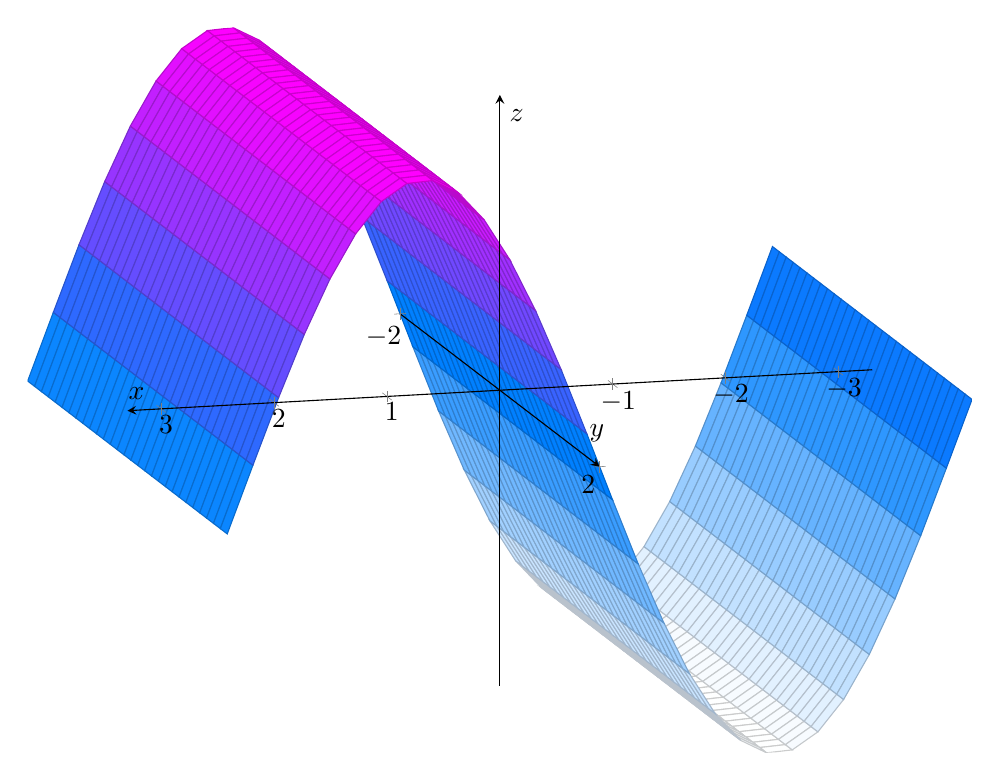
\begin{tikzpicture}
  \begin{axis}[
    view={165}{15},
    axis lines=center,
    xlabel={$x$},
    ylabel={$y$},
    zlabel={$z$},
    domain=-3.3:3.3,
    y domain=-2:2,
    samples=30,
    samples y=30,
    colormap/cool,
    z buffer=sort,
    axis on top,
    scale=1.75,
    ztick={-1,1}
  ]
    \addplot3[surf] {sin(deg(x)};
    \end{axis}
\end{tikzpicture}
\end{center}

\newpage

\noindent (b)
\begin{center}
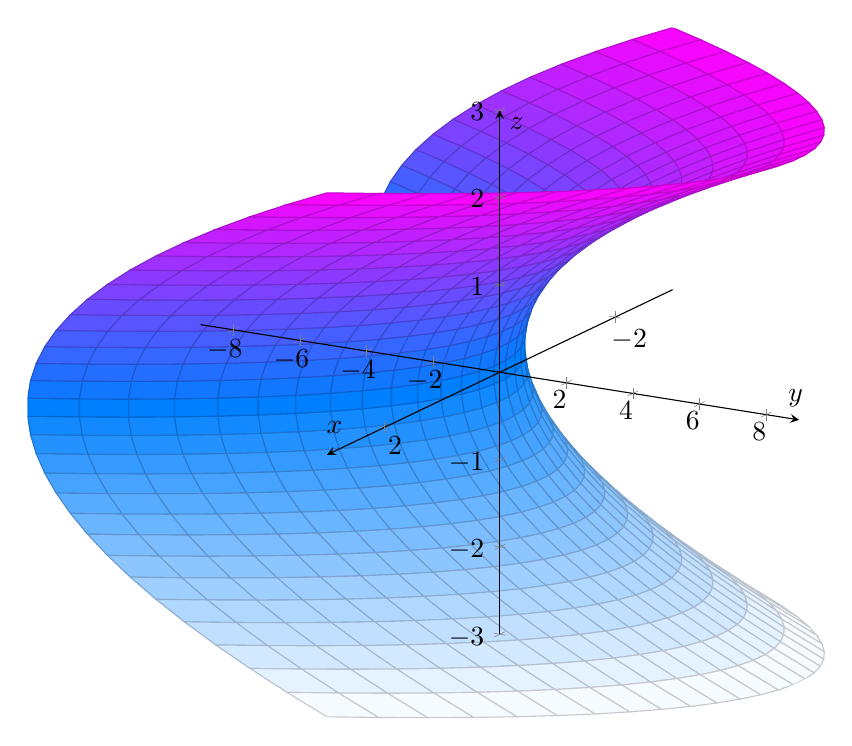
\begin{tikzpicture}
  \begin{axis}[
    view={120}{20},
    axis lines=center,
    xlabel={$x$},
    ylabel={$y$},
    zlabel={$z$},
    domain=-3:3,
    y domain=-3:3,
    samples=30,
    samples y=30,
    colormap/cool,
    z buffer=sort,
    axis on top,
    scale=1.75
  ]
    \addplot3[surf]({x}, {y^2 - x^2}, {y});
  \end{axis}
\end{tikzpicture}
\end{center}

\hfill

\noindent 5. Apply the Two-Path Test.

\[y=x\implies\lim_{(x,y)\to(0,0)}\frac{xy^2}{x^2+y^4}=\lim_{x\to0}\frac{x^3}{x^2+x^4}=\lim_{x\to0}\frac{x}{1+x^2}=\frac01=0\]
\[x=y^2\implies\lim_{(x,y)\to(0,0)}\frac{xy^2}{x^2+y^4}=\lim_{y\to0}\frac{y^4}{2y^4}=\frac12\]

\hfill

\noindent Since $0\neq\dfrac12$, by the Two-Path Test, the limit does not exist.

\hfill

\noindent 6.

\hfill

\noindent (a) Apply the product rule.

\[\frac\partial{\partial T}\left[\left(P+\frac A{V^2}\right)(V-B)\right]=\frac\partial{\partial T}\left(kT\right)\]

\[\left(\frac{\partial P}{\partial T}-\frac{2A}{V^3}\cdot\frac{\partial V}{\partial T}\right)(V-B)+\left(P+\frac A{V^2}\right)\left(\frac{\partial V}{\partial T}\right)=k\]

\[(V-B)\frac{\partial P}{\partial T}+\frac{\partial V}{\partial T}\left(-\frac{2A}{V^2}+\frac{2AB}{V^3}\right)+\frac{\partial V}{\partial T}\left(P+\frac{A}{V^2}\right)=k\]

\[\boxed{\frac{\partial V}{\partial T}=\frac{k+(B-V)\dfrac{\partial P}{\partial T}}{P+\dfrac{2AB}{V^3}-\dfrac{A}{V^2}}}\]

\hfill

\noindent (b) Apply the product rule again.

\[\frac\partial{\partial V}\left[\left(P+\frac A{V^2}\right)(V-B)\right]=\frac\partial{\partial V}\left(kT\right)\]

\[\left(\frac{\partial P}{\partial V}-\frac{2A}{V^3}\right)(V-B)+\left(P+\frac A{V^2}\right)\cdot1=k\frac{\partial T}{\partial V}\]

\[(V-B)\frac{\partial P}{\partial V}-\frac{2A}{V^2}+\frac{2AB}{V^3}=k\frac{\partial T}{\partial V}-P-\frac A{V^2}\]

\[\boxed{\frac{\partial P}{\partial V}=\frac{k\dfrac{\partial T}{\partial V}-P+\dfrac A{V^2}-\dfrac{2AB}{V^3}}{V-B}}\]

\hfill

\noindent 7. $z=z(x,y),\:x=x(t)$ and $y=y(t)$. Apply the chain rule.

\begin{align*}\frac{dz}{dt}&=\frac{\partial z}{\partial x}\cdot\frac{dx}{dt}+\frac{\partial z}{\partial y}\cdot\frac{dy}{dt}=(2x-y)(-\sin t)+(2y-x)(\cos t)\\\\&=(2\cos t-\sin t)(-\sin t)+(2\sin t-\cos t)(\cos t)=\sin^2t-\cos^2t=-\cos2t\end{align*}

\hfill

\noindent The result is then

\[\left.\frac{dz}{dt}\right|_{t=0}=-\cos0=\boxed{-1}\]

\hfill

\noindent 8. Let $f(x,y,z)=x^2+y^2-z=0$ and $g(x,y,z)=2x^2+2y^2+z^2=8$ be level surfaces. The tangent line is perpendicular to both $\nabla f$ and $\nabla g$ at $P$.

\[\nabla f=\left\langle2x,2y,-1\right\rangle,\qquad\nabla g=\left\langle4x,4y,2z\right\rangle\]
\[\nabla f(P)=\left\langle-2,2,-1\right\rangle,\qquad\nabla g(P)=\left\langle-4,4,4\right\rangle\]

\begin{align*}\mathbf{T}&=\nabla f\times\nabla g=\left|\begin{array}{ccc}
\mathbf{i}&\mathbf{j}&\mathbf{k}\\
-2&2&-1\\
-4&4&4
\end{array}\right|=\mathbf{i}\left|\begin{array}{cc}
2&-1\\4&4
\end{array}\right|-\mathbf{j}\left|\begin{array}{cc}
-2&-1\\-4&4
\end{array}\right|+\mathbf{k}\left|\begin{array}{cc}
-2&2\\-4&4
\end{array}\right|\\\\&=(2\cdot4-4\cdot(-1))\mathbf{i}-(-2\cdot4-(-4)\cdot(-1))\mathbf{j}+(-2\cdot4-2\cdot(-4))\mathbf{k}=12\mathbf i+12\mathbf j\end{align*}

\hfill

\noindent The parametric equations for the tangent line is

\[\boxed{\left.\begin{array}{l}
x=-1+12t\\
y=1+12t\\
z=2
\end{array}\right\}\quad t\in\mathbb{R}}\]

\newpage


\begin{center}
2022-2023 Spring Midterm (08/05/2023) Solutions\\
(Last update: 25/08/2025 23:50)
\end{center}

\noindent 1.

\hfill

\noindent (a)
\begin{center}
\begin{tikzpicture}
  \begin{axis}[
  title={Plane $x=0$},
    xlabel=$y$, ylabel=$z$,
    xtick=\empty, ytick=\empty,
    samples=50,
    axis lines=middle,
    clip=true,
    scale=1,
    enlargelimits=true
    ]
    \addplot[domain=-5:-2, blue] {sqrt(x^2/4-1)};
    \addplot[domain=2:5, blue] {sqrt(x^2/4-1)};
    \addplot[domain=-5:-2, blue] {-sqrt(x^2/4-1)};
    \addplot[domain=2:5, blue] {-sqrt(x^2/4-1)};

    \node[blue] at (2.1,-2) {$\dfrac{y^2}4-z^2=1$};
  \end{axis}
\end{tikzpicture}\hspace{1em}
\begin{tikzpicture}
  \begin{axis}[
  title={Plane $y=0$},
    xlabel=$x$, ylabel=$z$,
    xtick=\empty, ytick=\empty,
    samples=50,
    axis lines=middle,
    clip=true,
    scale=1,
    enlargelimits=true
    ]
    \addplot[domain=-8:-4, red] {sqrt(x^2/16-1)};
    \addplot[domain=4:8, red] {sqrt(x^2/16-1)};
    \addplot[domain=-8:-4, red] {-sqrt(x^2/16-1)};
    \addplot[domain=4:8, red] {-sqrt(x^2/16-1)};

    \node[red] at (3.5,-1.5) {$\dfrac{x^2}{16}-z^2=1$};
  \end{axis}
\end{tikzpicture}

\hfill

\begin{tikzpicture}
  \begin{axis}[
  title={Plane $z=0$},
  axis equal image,
    xlabel=$x$, ylabel=$y$,
    xtick=\empty, ytick=\empty,
    samples=200,
    axis lines=middle,
    clip=true,
    scale=1,
    enlargelimits=true
    ]
    \addplot[domain=-4:4, orange] {4*sqrt(1-x^2/16)};
    \addplot[domain=-4:4, orange] {-4*sqrt(1-x^2/16)};

    \node[orange] at (1.9,1.1) {\small $\dfrac{x^2}{16}+\dfrac{y^2}4=1$};
  \end{axis}
\end{tikzpicture}\hspace{1em}
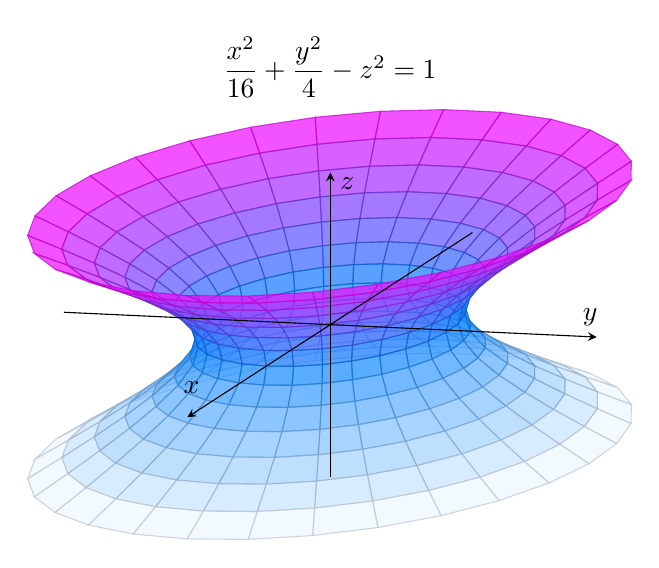
\begin{tikzpicture}
  \begin{axis}[
    title={$\dfrac{x^2}{16}+\dfrac{y^2}4-z^2=1$},
    title style={yshift=-20pt},
      view={105}{10},
      axis lines=center,
      axis equal image,
      xlabel={$x$},
      ylabel={$y$},
      zlabel={$z$},
      domain=0:2*pi,
      y domain=-2:2,
      samples=30,
      samples y=15,
      zmin=-2.5, zmax=2.5,
      colormap/cool,
      axis on top,
      scale=2.5,
      xtick=\empty, ytick=\empty, ztick=\empty,
      z buffer=sort,
    ]
    \addplot3[
      surf,
      opacity=0.7
    ]
    ( {4*sqrt(1+y^2)*cos(deg(x))},
      {2*sqrt(1+y^2)*sin(deg(x))},
      {y} );
  \end{axis}
\end{tikzpicture}
\end{center}

\hfill

\noindent (b)
\begin{center}
\begin{tikzpicture}
  \begin{axis}[
  title={Plane $x=0$},
    xlabel=$y$, ylabel=$z$,
    xtick=\empty, ytick=\empty,
    samples=50,
    axis lines=middle,
    clip=true,
    scale=1,
    enlargelimits=true
    ]
    \addplot[domain=-5:5, blue] {x^2/4-6};

    \node[blue] at (1.9,-1.8) {$z=\dfrac{y^2}4-6$};
  \end{axis}
\end{tikzpicture}\hspace{1em}
\begin{tikzpicture}
  \begin{axis}[
  title={Plane $y=0$},
    xlabel=$x$, ylabel=$z$,
    xtick=\empty, ytick=\empty,
    samples=50,
    axis lines=middle,
    clip=true,
    scale=1,
    enlargelimits=true
    ]
    \addplot[domain=-5:5, red] {x^2/4-6};

    \node[red] at (1.9,-1.8) {$z=\dfrac{x^2}4-6$};
  \end{axis}
\end{tikzpicture}

\begin{tikzpicture}
  \begin{axis}[
  title={Plane $z=0$},
  axis equal image,
    xlabel=$x$, ylabel=$y$,
    xtick=\empty, ytick=\empty,
    samples=300,
    axis lines=middle,
    clip=true,
    scale=1,
    enlargelimits=true
    ]
    \addplot[domain=-2*sqrt(6):2*sqrt(6), orange] {sqrt(24-x^2)};
    \addplot[domain=-2*sqrt(6):2*sqrt(6), orange] {-sqrt(24-x^2)};

    \node[orange] at (2.4,0.8) {\small $y^2=24-x^2$};
  \end{axis}
\end{tikzpicture}\hspace{1em}
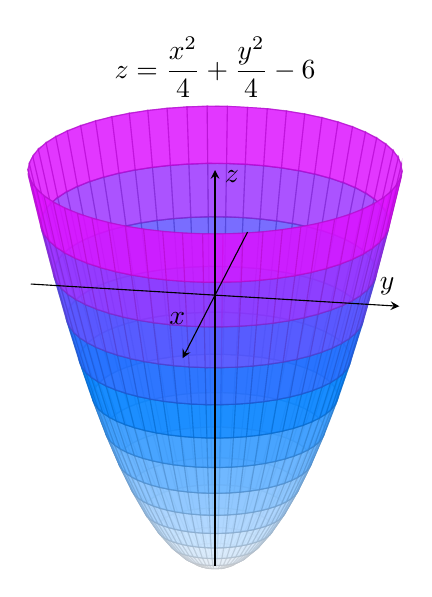
\begin{tikzpicture}
  \begin{axis}[
    title={$\displaystyle z=\frac{x^2}4+\frac{y^2}4-6$},
    title style={yshift=-10pt},
      view={100}{20},
      axis lines=center,
      axis equal image,
      xlabel={$x$},
      ylabel={$y$},
      zlabel={$z$},
      domain=0:2*pi,
      y domain=-2.25:2.25,
      samples=30,
      samples y=30,
      colormap/cool,
      axis on top,
      scale=1.5,
      xtick=\empty, ytick=\empty, ztick=\empty,
      z buffer=sort,
    ]
    \addplot3[
      surf,
      opacity=0.6
    ]
    ( {y*cos(deg(x))},
      {y*sin(deg(x))},
      {y^2-2*sqrt(3)} );
  \end{axis}
\end{tikzpicture}
\end{center}

\hfill

\noindent 2. Apply the Two-Path Test.

\[x=y\implies\lim_{(x,y)\to(0,0)}\frac{y^3\sqrt x}{2\left(x^2+y^4\right)}=\lim_{x\to0}\frac{x^{7/2}}{2\left(x^2+x^4\right)}=\lim_{x\to0}\frac{x^{3/2}}{2\left(1+x^2\right)}=\frac02=0\]
\[x=y^2\implies\lim_{(x,y)\to(0,0)}\frac{y^3\sqrt x}{2\left(x^2+y^4\right)}=\lim_{y\to0}\frac{y^4}{4y^4}=\lim_{y\to0}\frac14=\frac14\]

\hfill

\noindent Since $0\neq\dfrac14$, by the Two-Path Test, the limit does not exist.

\hfill

\noindent 3. Let $f(x,y,z)=xz^2-2xy+y^2=2$ and $g(x,y,z)=xz-x^2y+z^2=1$ be the level surfaces. The cross product of the gradient of these functions give us the vector that is parallel to the line of intersection. Compute the gradients.

\[\nabla f=\left\langle z^2-2y,\:-2x+2y,\:2xz\right\rangle,\quad \nabla g=\left\langle z-2xy,\:-x^2,\: x+2z\right\rangle\]
\[\nabla f\,|_{\left(0,\,\sqrt2,\,1\right)}=\left\langle1-2\sqrt2,\:2\sqrt2,\:0\right\rangle,\quad \nabla g\,|_{\left(0,\,\sqrt2,\,1\right)}=\left\langle1,\:0,\:2\right\rangle\]

\hfill

\noindent Find the cross product.

\begin{align*}\mathbf{n}&=\nabla f\times \nabla g=\left|\begin{array}{ccc}
\mathbf{i}&\mathbf{j}&\mathbf{k}\\
1-2\sqrt2&2\sqrt2&0\\
1&0&2
\end{array}\right|\\\\&=\mathbf{i}\left|\begin{array}{cc}
2\sqrt2&0\\0&2
\end{array}\right|-\mathbf{j}\left|\begin{array}{cc}
1-2\sqrt2&0\\1&2
\end{array}\right|+\mathbf{k}\left|\begin{array}{cc}
1-2\sqrt2&2\sqrt2\\1&0
\end{array}\right|\\\\&=\left(2\sqrt2\cdot2-0\cdot0\right)\mathbf{i}-\left[\left(1-2\sqrt2\right)\cdot2-0\cdot1\right]\mathbf{j}+\left[\left(1-2\sqrt2\right)\cdot0-2\sqrt2\cdot1\right)\mathbf{k}\\\\&=4\sqrt2\,\mathbf{i}+\left(4\sqrt2-2\right)\,\mathbf{j}+-2\sqrt2\,\mathbf{k}\end{align*}

\hfill

\noindent The line of intersection is the normal line of the plane. Therefore, $\mathbf n$ is the normal vector of the plane. The equation of the plane with the normal vector $\mathbf n$ and containing the point $P(x_0,y_0,z_0)$ is

\[n_1(x-x_0)+n_2(y-y_0)+n_3(z-z_0)=0\]

\hfill

\noindent Therefore, the equation for this plane is

\[4\sqrt2(x-0)+\left(4\sqrt2-2\right)(y-1)-2\sqrt2(z-2)=0\]

\[\boxed{2x\sqrt2+y\left(2\sqrt2-1\right)-z\sqrt2+1=0}\]

\hfill

\noindent 4. Apply the chain rule.

\[\frac{\partial w}{\partial s}=\frac{\partial w}{\partial x}\cdot\frac{\partial x}{\partial s}+\frac{\partial w}{\partial y}\cdot\frac{\partial y}{\partial s}+\frac{\partial w}{\partial z}\cdot\frac{\partial z}{\partial s}\]

\hfill

\noindent Compute the partial derivatives.

\[\frac{\partial w}{\partial x}=y\ln\left(1+\sqrt{x^2+y^2}\right)+xy\cdot\frac1{1+\sqrt{x^2+y^2}}\cdot\left(\frac{x}{\sqrt{x^2+y^2}}\right)+z\]
\[\frac{\partial w}{\partial y}=x\ln\left(1+\sqrt{x^2+y^2}\right)+xy\cdot\frac1{1+\sqrt{x^2+y^2}}\cdot\left(\frac{y}{\sqrt{x^2+y^2}}\right),\quad \frac{\partial w}{\partial z}=x\]

\[\frac{\partial x}{\partial s}=1,\quad\frac{\partial y}{\partial s}=\mathrm{e}^s,\quad\frac{\partial z}{\partial s}=\frac{2s}{s^2+t}\]

\begin{align*}\frac{\partial w}{\partial s}=&\left[y\ln\left(1+\sqrt{x^2+y^2}\right)+xy\cdot\frac1{1+\sqrt{x^2+y^2}}\cdot\left(\frac{x}{\sqrt{x^2+y^2}}\right)+z\right]\cdot1\\\\&+\left[x\ln\left(1+\sqrt{x^2+y^2}\right)+xy\cdot\frac1{1+\sqrt{x^2+y^2}}\cdot\left(\frac{y}{\sqrt{x^2+y^2}}\right)\right]\cdot\mathrm{e}^s+\frac{2xs}{s^2+t}\end{align*}

\hfill

\noindent Write in terms of $s$ and $t$ rigorously.

\[\boxed{\begin{array}{ll}\dfrac{\partial w}{\partial s}=&
\mathrm{e}^s\ln\left(1+\sqrt{(t+s)^2+\mathrm{e}^{2s}}\right)+\dfrac{(t+s)^2\cdot\mathrm{e}^s}{\sqrt{(t+s)^2+\mathrm{e}^{2s}}+(t+s)^2+\mathrm{e}^{2s}}+\ln\left(s^2+t\right)\\\\&+(t+s)\mathrm{e}^s\ln\left(1+\sqrt{(t+s)^2+\mathrm{e}^{2s}}\right)+\dfrac{(t+s)\cdot\mathrm{e}^{3s}}{\sqrt{(t+s)^2+\mathrm{e}^{2s}}+(t+s)^2+\mathrm{e}^{2s}}\\\\&+\dfrac{2s(t+s)}{s^2+t}
\end{array}}\]

\hfill

\noindent 5. Let $f(x,y)=\tan\left(xy^2\right)$. The total differential of $f$ is

\[df=f_x\,dx+f_y\,dy=\sec^2\left(xy^2\right)\cdot y^2\,dx+\sec^2\left(xy^2\right)\cdot2xy\,dy\]

\hfill

\noindent Since $x=0.97\approx1$ and $y=2.05\approx2$, we may approximate the value of $\tan\left(0.97\cdot2.05^2\right)$ near $\tan\left(1\cdot 2^2\right)=\tan4$. Take $x=1,\:y=2,\:dx=0.97-1=-0.03,\:dy=2.05-2=0.05$.

\[df=\sec^24\cdot4\cdot(-0.03)+\sec^24\cdot4\cdot(0.05)=0.08\sec^24\]

\hfill

\noindent Since $f(x+\Delta x,\:y+\Delta y)\approx f(x,y)+df$, the value of $\tan\left(0.97\cdot2.05^2\right)$ is approximately

\[\boxed{\tan4+0.08\sec^24}\]

\hfill

\noindent 6. The function $f$ has the minimum rate of change if the gradient vector of $f$ and the unit direction vector $\mathbf u$ are antiparallel. That is, they have opposite directions.

\[\nabla f=\left\langle\frac1{2\sqrt{x+yz}},\frac z{2\sqrt{x+yz}},\frac y{2\sqrt{x+yz}}\right\rangle\]

\[\left(\nabla f\cdot \mathbf u\right)_{\text{min}}=\left|\nabla f\right||u|\cos\pi=-|\nabla f|\]

\[\nabla f|_{(1,1,3)}=\left\langle\frac14,\frac34,\frac14\right\rangle\implies-|\nabla f|=-\sqrt{\left(\frac14\right)^2+\left(\frac34\right)^2+\left(\frac14\right)^2}=-\frac{\sqrt{11}}4\]

\hfill

\noindent Since $\mathbf u$ has the opposite direction to that of the gradient, we may also find the components of $\mathbf u$.

\[\mathbf{u}=-\frac{\nabla f}{|\nabla f|}=-\frac{\left\langle\frac14,\frac34,\frac14\right\rangle}{\frac{\sqrt{11}}4}=\left\langle-\frac1{\sqrt{11}},-\frac3{\sqrt{11}},-\frac1{\sqrt{11}}\right\rangle\]

\[\boxed{\text{The minimum rate of change: }{-\frac{\sqrt{11}}4},\text{ the direction vector:}\left\langle-\frac1{\sqrt{11}},-\frac3{\sqrt{11}},-\frac1{\sqrt{11}}\right\rangle}\]

\hfill

\noindent 7. $f$ is continuous on a bounded and closed set on $\mathbb R$. By the Extreme Value Theorem, the extrema must exist in the region or on the boundary.

\hfill

\noindent First, determine where $f_x=f_y=0$ to find the critical points.

\[f_x=2x-y,\quad f_y=1-x\]
\[f_x=f_y=0\implies2x-y=0,\quad1-x=0\implies x=1,\quad y=2\]
\[f(1,2)=5\]

\hfill

\noindent Take a look at the boundary. From $(0,0)$ to $(4,0)$, we have $y=0$.

\[y=0\implies f(x,0)=x^2+4\quad\rightarrow\quad\frac d{dx}\left(x^2-4\right)=2x=0\implies x=0\]
\[f(0,0)=4\]

\hfill

\noindent From $(0,0)$ to $(0,4)$, we have $x=0$.

\[x=0\implies f(0,y)=y+4\quad\rightarrow\quad\frac d{dy}\left(y+4\right)=1\neq0\]

\hfill

\noindent From $(4,0)$ to $(0,4)$, we have $x=y$.

\[y=4-x\implies f(x,4-x)=x^2+(4-x)-x(4-x)+4=2x^2-5x+8\]

\[\frac d{dx}\left(2x^2-5x+8\right)=4x-5=0\implies x=\frac54,\quad y=\frac{11}4\]
\[f\left(\frac54,\frac{11}4\right)=\frac{39}8\]

\hfill

\noindent We also have $f(0,0)=5,\:f(4,0)=20,\:f(0,4)=8$ from the vertices of the triangular region.

\hfill

\noindent Compare all the values $f(0,0),\:f(1,2),\:f(4,0),\:f(0,4),\:f\left(\frac54,\frac{11}4\right)$.

\[\boxed{\text{Absolute minimum: }f(0,0)=4,\quad \text{absolute maximum: } f(4,0)=20.}\]

\newpage


\begin{center}
2023-2024 Spring Midterm (26/04/2024) Solutions\\
(Last update: 27/08/2025 23:24)
\end{center}

\noindent 1.

\hfill

\noindent (a)
\begin{center}
\begin{tikzpicture}
  \begin{axis}[
  title={Plane $x=0$},
    xlabel=$y$, ylabel=$z$,
    xtick=\empty, ytick=\empty,
    samples=30,
    axis lines=middle,
    clip=true,
    scale=1,
    enlargelimits=true
    ]
    \addplot[domain=-1:0.8, blue] {e^x};

    \node[blue] at (0.5,1) {$z=\mathrm{e}^y$};
  \end{axis}
\end{tikzpicture}\hspace{1em}
\begin{tikzpicture}
  \begin{axis}[
  title={Plane $y=0$},
    xlabel=$x$, ylabel=$z$,
    xtick=\empty, ytick=\empty,
    axis lines=middle,
    samples=30,
    clip=true,
    ymin=0, ymax=2,
    scale=1,
    enlargelimits=true
    ]
    \addplot[domain=-2:2, red, thick] {1};

    \node[red] at (1.5,1.5) {$z=1$};
  \end{axis}
\end{tikzpicture}

\hfill

\begin{tikzpicture}
  \begin{axis}[
  title={Plane $z=0$ (No intersection)},
  axis equal image,
    xlabel=$x$, ylabel=$y$,
    xtick=\empty, ytick=\empty,
    xmin=-1, xmax=1,
    ymin=-1, ymax=1,
    axis lines=center,
    clip=true,
    scale=1,
    enlargelimits=true
    ]
  \end{axis}
\end{tikzpicture}\hspace{1em}
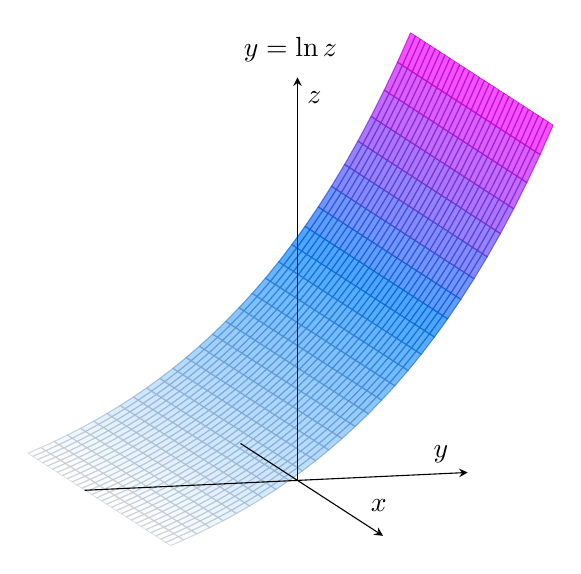
\begin{tikzpicture}
  \begin{axis}[
    title={$y=\ln z$},
    title style={yshift=-20pt},
      view={75}{10},
      axis lines=center,
      axis equal image,
      xlabel={$x$},
      ylabel={$y$},
      zlabel={$z$},
      domain=-1:1.5,
      y domain=-1:0.8,
      samples=30,
      samples y=30,
      colormap/cool,
      axis on top,
      scale=1.25,
      xtick=\empty, ytick=\empty, ztick=\empty,
      z buffer=sort,
    ]
    \addplot3[
      surf,
      opacity=0.7
    ]
    ( {x},
      {y},
      {e^y} );
  \end{axis}
\end{tikzpicture}
\end{center}

\hfill

\noindent (b)
\begin{center}
\begin{tikzpicture}
  \begin{axis}[
  title={Plane $x=0$},
    xlabel=$y$, ylabel=$z$,
    xtick=\empty, ytick=\empty,
    samples=30,
    axis lines=middle,
    clip=true,
    scale=1,
    enlargelimits=true
    ]
    \addplot[domain=-2:2, blue] {sqrt(2*x^2/3+1/3)};
    \addplot[domain=-2:2, blue] {-sqrt(2*x^2/3+1/3)};
    
    \node[blue] at (1.25,-0.4) {$2y^2+1=3z^2$};
  \end{axis}
\end{tikzpicture}\hspace{1em}
\begin{tikzpicture}
  \begin{axis}[
  title={Plane $y=0$},
    xlabel=$x$, ylabel=$z$,
    xtick=\empty, ytick=\empty,
    samples=30,
    axis lines=middle,
    clip=true,
    scale=1,
    enlargelimits=true
    ]
    \addplot[domain=-2:2, red] {sqrt(x^2/3+1/3)};
    \addplot[domain=-2:2, red] {-sqrt(x^2/3+1/3)};
    
    \node[red] at (1.25,-0.4) {$x^2+1=3z^2$};
  \end{axis}
\end{tikzpicture}

\begin{tikzpicture}
  \begin{axis}[
  title={Plane $z=0$ (No intersection)},
  axis equal image,
    xlabel=$x$, ylabel=$y$,
    xtick=\empty, ytick=\empty,
    xmin=-1, xmax=1,
    ymin=-1, ymax=1,
    axis lines=center,
    clip=true,
    scale=1,
    enlargelimits=true
    ]
  \end{axis}
\end{tikzpicture}\hspace{1em}
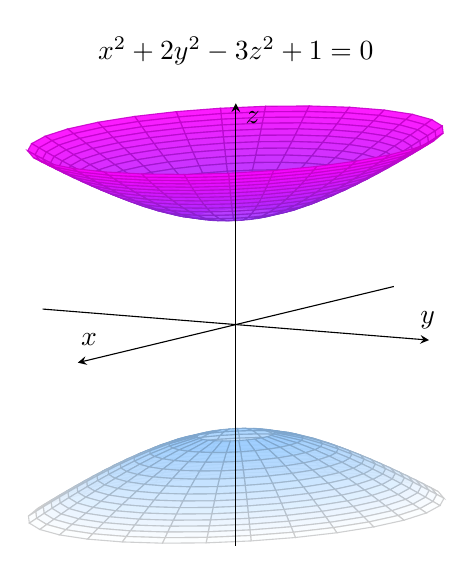
\begin{tikzpicture}
  \begin{axis}[
  title={$x^2+2y^2-3z^2+1=0$},
    title style={yshift=-15pt},
      view={120}{8},
      axis lines=center,
      axis equal image,
      xlabel={$x$},
      ylabel={$y$},
      zlabel={$z$},
      domain=0:2*pi,
      y domain=-2:2,
      samples=30,
      samples y=30,
      colormap/cool,
      axis on top,
      scale=1.6,
      xtick=\empty, ytick=\empty, ztick=\empty,
      z buffer=sort,
      enlargelimits=true,
    ]
    \addplot3[
      surf,
      opacity=0.9
    ]
    ( {sqrt(y)*cos(deg(x))},
      {1/sqrt(2))*sqrt(y)*sin(deg(x))},
      {(1/sqrt(3))*sqrt(y+1)} );
    \addplot3[
      surf,
      opacity=0.9
    ]
    ( {-sqrt(y)*cos(deg(x))},
      {-1/sqrt(2))*sqrt(y)*sin(deg(x))},
      {-(1/sqrt(3))*sqrt(y+1)} );
  \end{axis}
\end{tikzpicture}
\end{center}

\hfill

\noindent 2. The $\epsilon-\delta$ definition is the formal way of calculating the limit of a function at a point $(x_0,y_0)$. According to the definition, for every $\epsilon>0$, there exists a $\delta$ such that

\[0<\sqrt{(x-x_0)^2+(y-y_0)^2}<\delta\implies\left|f(x,y)-L\right|<\epsilon,\]

\hfill

\noindent where $L$ is the limit.

\hfill

\noindent Then for every $\epsilon>0$, there exists a $\delta$ such that

\[0<\sqrt{x^2+y^2}<\delta\implies\left|2x^2+y^2\right|<\epsilon.\]

\[\left|2x^2+y^2\right|\leq2x^2+y^2\qquad\left[x^2\geq0,\quad y^2\geq0\right]\]

\[2x^2+y^2\leq2x^2+2y^2=2\left(x^2+y^2\right)\leq2\delta^2\qquad\left[\sqrt{x^2+y^2}<\delta\implies  x^2+y^2<\delta^2\right]\]

\hfill

\noindent Let $\delta=\sqrt{\dfrac{\epsilon}2}$.

\[\left|2x^2+y^2\right|\leq2\left(x^2+y^2\right)<2\cdot\left(\sqrt{\frac{\epsilon}2}\right)^2=2\cdot\frac{\epsilon}2=\epsilon\]

\hfill

\noindent This shows that the limit is equal to $0$.

\hfill

\noindent 3. The coefficients of the parametrization variables have the same ratio. That is, they are parallel. Choose $P_1(3,3,3)$ on $l_1$ and $P_2(1,2,1)$ on $l_2$. The cross product of $\mathbf u=\left\langle3,-1,2\right\rangle$, which is parallel to the lines, and the vector $\mathbf v$ joining $P_1$ and $P_2$, where $\mathbf w=\left\langle3-1,\,3-2,\,3-1\right\rangle=\left\langle2,1,2\right\rangle$, gives us the normal of the plane.

\begin{align*}\mathbf n&=\mathbf{u}\times\mathbf{v}=\left|\begin{array}{ccc}
\mathbf{i}&\mathbf{j}&\mathbf{k}\\
3&-1&2\\
2&1&2
\end{array}\right|=\mathbf{i}\left|\begin{array}{cc}
-1&2\\1&2
\end{array}\right|-\mathbf{j}\left|\begin{array}{cc}
3&2\\2&2
\end{array}\right|+\mathbf{k}\left|\begin{array}{cc}
3&-1\\2&1
\end{array}\right|\\\\&=(-1\cdot2-1\cdot2)\mathbf{i}-(3\cdot2-2\cdot2)\mathbf{j}+(3\cdot1-2\cdot(-1))\mathbf{k}=-4\mathbf i-2\mathbf j+5\mathbf k\end{align*}

\hfill

\noindent Using the definition $\mathbf{n}\cdot\overrightarrow{PP_1}=0$, where $P$ is a point on the plane, the equation of the plane is

\begin{align*}\mathbf{n}\cdot\overrightarrow{PP_1}=0&\implies\left\langle-4,-2,5\right\rangle\cdot\left\langle x-3,\,y-3,\,z-3\right\rangle=0\\\\&\implies-4(x-3)-2(y-3)+5(z-3)=0\implies\boxed{-4x-2y+5z+3=0}\end{align*}

\hfill

\noindent 4.

\hfill

\noindent (i) Use the definition of the partial derivative.

\begin{align*}f_x|_{(0,0)}&=\lim_{h\to0}\frac{f(0+h,0)-f(0,0)}h=\lim_{h\to0}\frac{\dfrac{(0+h)^2\cdot\mathrm{e}^{(0+h)^2+0}}{(0+h)^2+0^2}}{h}=\lim_{h\to0}\frac{\mathrm{e}^{h^2}}{h}\\\\&=\infty\:(f_x\:\text{does not exist})\end{align*}

\[f_y|_{(0,0)}=\lim_{h\to0}\frac{f(0,0+h)-f(0,0)}h=\lim_{h\to0}\frac{\dfrac{0^2\cdot\mathrm{e}^{0^2+(0+h)}}{0^2+(0+h)^2}}{h}=\lim_{h\to0}\frac{0}{h}=0\]

\hfill

\noindent (ii) $f_y$ is a finite number. However, since $f_x$ does not exist, $f$ is not differentiable at $(0,0)$.

\hfill

\noindent 5. $u$ and $v$ are functions of $x$ and $y$. $x$ and $y$ are functions of $r$ and $\theta$. Use the chain rule.

\[\frac{\partial u}{\partial r}=\frac{\partial u}{\partial x}\cdot\frac{\partial x}{\partial r}+\frac{\partial u}{\partial y}\cdot\frac{\partial y}{\partial r}=u_x\cdot\cos\theta+u_y\cdot\sin\theta=v_y\cos\theta-v_x\sin\theta\]

\[\frac{\partial v}{\partial\theta}=\frac{\partial v}{\partial x}\cdot\frac{\partial x}{\partial\theta}+\frac{\partial v}{\partial y}\cdot\frac{\partial y}{\partial\theta}\implies\frac1r\frac{\partial v}{\partial\theta}=\frac1r\left(-v_x\cdot r\sin\theta+v_y\cdot r\cos\theta\right)=-v_x\sin\theta+v_y\cos\theta\]

\[\frac{\partial u}{\partial r}=-v_x\sin\theta+v_y\cos\theta=\frac1r\frac{\partial v}{\partial\theta}\]

\hfill

\[\frac{\partial v}{\partial r}=\frac{\partial v}{\partial x}\cdot\frac{\partial x}{\partial r}+\frac{\partial v}{\partial y}\cdot\frac{\partial y}{\partial r}=v_x\cdot\cos\theta+v_y\cdot\sin\theta=-u_y\cos\theta+u_x\sin\theta\]

\[\frac{\partial u}{\partial\theta}=\frac{\partial u}{\partial x}\cdot\frac{\partial x}{\partial\theta}+\frac{\partial u}{\partial y}\cdot\frac{\partial y}{\partial\theta}\implies-\frac1r\frac{\partial u}{\partial\theta}=-\frac1r\left(-u_x r\sin\theta+u_y r\cos\theta\right)=u_x\sin\theta-u_y\cos\theta\]

\[\frac{\partial v}{\partial r}=u_x\sin\theta-u_y\cos\theta=-\frac1r\frac{\partial u}{\partial \theta}\]

\hfill

\noindent 6. The function $f$ has the maximum rate of change if the gradient vector of $f$ and the unit direction vector $\mathbf u$ are in the same direction. Apply the quotient rule to compute the gradient of $f$.
\[\nabla f=\left\langle\frac{\left(2^{xy}\cdot y\cdot\ln2\right)\cdot x-2^{xy}\cdot(1)}{x^2},\,2^{xy}\cdot\ln2\right\rangle=\left\langle\frac{2^{xy}\left(yx\ln2-1\right)}{x^2},\,2^{xy}\cdot\ln2\right\rangle\]

\[\left(\nabla f\cdot\mathbf u\right)_{\text{max}}=\left|\nabla f\right||u|\cos0=|\nabla f|\]

\begin{align*}\nabla f|_{(1,1)}&=\left\langle2\ln2-2,\,2\ln2\right\rangle\implies|\nabla f|=\sqrt{\left(2\ln2-2\right)^2+\left(2\ln2\right)^2}\\\\&=2\sqrt{2\ln^22-2\ln2+1}\end{align*}

\hfill

\noindent The unit direction vector $u$ is
\[\mathbf{u}=\frac{\nabla f}{|\nabla f|}=\frac{\left\langle2\ln2-2,\,2\ln2\right\rangle}{2\sqrt{2\ln^22-2\ln2+1}}=\left\langle\frac{\ln2-1}{\sqrt{2\ln^22-2\ln2+1}},\frac{\ln2}{\sqrt{2\ln^22-2\ln2+1}}\right\rangle\]

\[\boxed{\begin{array}{c}\text{The maximum rate of change: }{2\sqrt{2\ln^22-2\ln2+1}}\\[1em]\text{The direction vector:}\left\langle\dfrac{\ln2-1}{\sqrt{2\ln^22-2\ln2+1}},\dfrac{\ln2}{\sqrt{2\ln^22-2\ln2+1}}\right\rangle\end{array}}\]

\hfill

\noindent 7. Apply the chain rule.
\begin{align*}f_x&=(y+1)\left[1\cdot(x-y+3)+(x-1)\cdot1\right]=(y+1)(2x-y+2)\\\\&=2xy-y^2+2y+2x-y+2=-y^2+y+2xy+2x+2\end{align*}
\begin{align*}f_y&=(x-1)\left[1\cdot(x-y+3)+(y+1)\cdot(-1)\right]=(x-1)(x-2y+2)\\\\&=x^2-2xy+2x-x+2y-2=x^2-2xy+x+2y-2\end{align*}

\hfill

\noindent The critical points occur where one of the partial derivatives does not exist or $f_x=f_y=0$. $f_x$ and $f_y$ are continuous everywhere. Therefore, we may simply determine where $f_x=f_y=0$.

\begin{align*}f_x=f_y=0&\implies\left.\begin{array}{rc}
2xy-y^2+2y+2x-y+2=0&(1)\\
x^2-2xy+x+2y-2=0
\end{array}\right\}\quad x^2-y^2+3(x+y)=0\\\\&\implies(x-y)(x+y)+3(x+y)=0\implies(x-y+3)(x+y)=0\end{align*}

\hfill

\noindent We have two cases: $x+3=y$ or $x=-y$.

\begin{flalign*}\text{Case I}:x=-y&\overset{(1)}\implies-y^2-2y^2+y-2y+2=0\implies -3y^2-y+2=0\\\\&\implies
(2-3y)(y+1)=0\implies y_1=\frac23,\:y_2=-1&\end{flalign*}
\[y_1=\frac23\implies x_1=-\frac23\qquad y_2=-1\implies x_2=1\]

\begin{flalign*}\text{Case II}:x+3=y&\overset{(1)}\implies-(x+3)^2+2x(x+3)+x+3+2x+2=0\\\\&\implies-x^2-6x-9+2x^2+6x+3x+5=0\implies x^2+3x-4=0&\end{flalign*}
\[x_{3,4}=\frac{-3\pm\sqrt{9-4\cdot1\cdot(-4)}}{2\cdot1}=\frac{-3\pm5}2\implies x_3=-4,\:x_4=1\implies y_3=-1,\:y_4=4\]

\hfill

\noindent To classify these four critical points, apply the Second Derivative Test.

\[f_{xx}=2y+2,\quad f_{xy}=f_{yx}=2x-2y+1,\quad f_{yy}=-2x+2\]

\begin{flalign*}\left(-\frac23,\frac23\right)\rightarrow\left\{\:\begin{array}{l}
f_{xx}=\dfrac{10}3,\quad f_{xy}=-\dfrac53 ,\quad f_{yy}=\dfrac{10}3\\[1em]
\left|\begin{array}{cc}
\dfrac{10}3&-\dfrac{10}3\\[1em]
-\dfrac53 & \dfrac{10}3
\end{array}\right|=\dfrac{10}3\cdot\dfrac{10}3-\left(-\dfrac53\right)\cdot\left(-\dfrac53\right)=\dfrac{25}3,\quad f_{xx}=\dfrac{10}3>0
\end{array}\right.&&\end{flalign*}

\begin{flalign*}\left(1,-1\right)\rightarrow\left\{\:\begin{array}{l}
f_{xx}=0,\quad f_{xy}=5,\quad f_{yy}=0\\[1em]
\left|\begin{array}{cc}
0 & 5\\
5 & 0
\end{array}\right|=0\cdot0-5\cdot5=-25<0
\end{array}\right.&&\end{flalign*}

\begin{flalign*}\left(-4,-1\right)\rightarrow\left\{\:\begin{array}{l}
f_{xx}=0,\quad f_{xy}=-5,\quad f_{yy}=10\\[1em]
\left|\begin{array}{cc}
0 & -5\\
-5 & 10
\end{array}\right|=0\cdot10-(-5)\cdot(-5)=-25<0
\end{array}\right.&&\end{flalign*}

\begin{flalign*}\left(1,4\right)\rightarrow\left\{\:\begin{array}{l}
f_{xx}=10,\quad f_{xy}=5,\quad f_{yy}=0\\[1em]
\left|\begin{array}{cc}
10 & 5\\
5 & 0
\end{array}\right|=10\cdot0-5\cdot5=-25<0
\end{array}\right.&&\end{flalign*}

\[\boxed{\begin{array}{c}\text{A local minimum occurs at }\left(-\dfrac23,\dfrac23\right).\\\text{ Saddle points occur at } (1,-1), (-4,-1),\:\text{and}\:(1,4).\end{array}}\]

\newpage


\begin{center}
2024-2025 Spring Midterm (09/04/2025) Solutions\\
(Last update: 29/08/2025 01:59)
\end{center}

\noindent 1.

\hfill

\noindent (a) Determine whether the graph is symmetric about the $x$-axis.

\[(r,\theta)\rightarrow r=2\cos(3\theta),\qquad (r,-\theta)\rightarrow r=2\cos(-3\theta)=2\cos(3\theta)\]

\hfill

\noindent $(r,\theta)$ is on the graph, and the graph is symmetric about the $x$-axis. Determine whether the graph is symmetric about the origin.

\[(r,\theta)\rightarrow r=2\cos(3\theta),\qquad (r,\theta+\pi)\rightarrow r=2\cos(-3(\theta+\pi))=-2\cos(3\theta)\]

\hfill

\noindent $(r,\theta+\pi)$ is not on the graph, and the graph is not symmetric about the origin. Determine whether the graph is symmetric about the $y$-axis.

\[(r,\theta)\rightarrow r=2\cos(3\theta),\qquad (r,\theta-\pi)\rightarrow r=2\cos(-3(\theta-\pi))=-2\cos(3\theta)\]

\hfill

\noindent $(r,\theta-\pi)$ is not on the graph, and the graph is not symmetric about the $y$-axis. 

\begin{center}
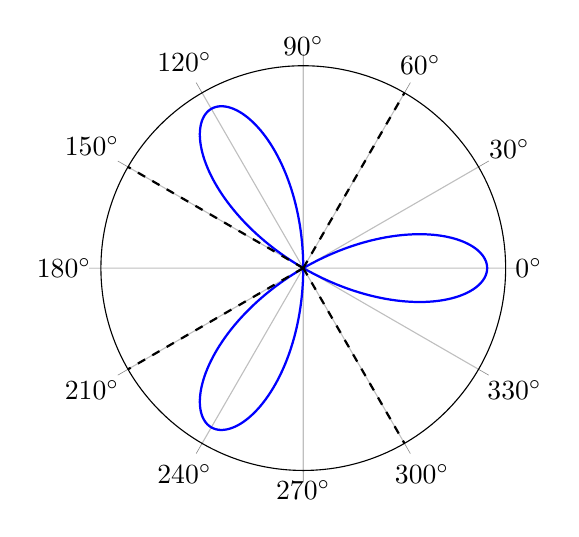
\begin{tikzpicture}
  \begin{polaraxis}[ytick=\empty, axis y line=none, xticklabel=$\pgfmathprintnumber{\tick}^\circ$,      scale=0.75,]
    \addplot [
      domain=0:2*pi,
      samples=300,
      thick,
      blue,
      data cs=polarrad,
    ] {2*cos(deg(3*x))};

    \draw[black, thick, dashed] (axis cs: 60,0) -- (axis cs: 60,2.5);
    \draw[black, thick, dashed] (axis cs: -60,0) -- (axis cs: -60,2.5);
    \draw[black, thick, dashed] (axis cs: 150,0) -- (axis cs: 150,2.5);
    \draw[black, thick, dashed] (axis cs: 210,0) -- (axis cs: 210,2.5);

  \end{polaraxis}
\end{tikzpicture}
\end{center}

\noindent (b) It is sufficient to calculate the area of the upper half of the leaf right to the $y$-axis and multiply the result by six.

\begin{center}
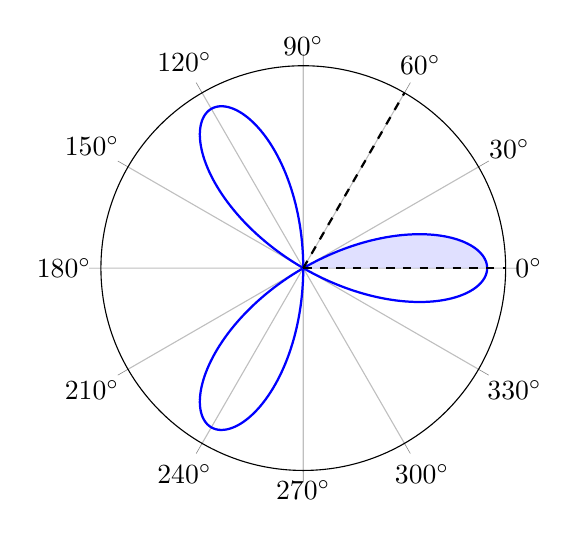
\begin{tikzpicture}
  \begin{polaraxis}[ytick=\empty, axis y line=none, xticklabel=$\pgfmathprintnumber{\tick}^\circ$,      scale=0.75,]
    \addplot [
      domain=0:2*pi,
      samples=300,
      thick,
      blue,
      data cs=polarrad,
    ] {2*cos(deg(3*x))};
    
    \addplot [
      domain=0:pi/6,
      draw=none,
      data cs=polarrad,
      name path=B
    ] {2*cos(deg(3*x))};
    
    \addplot [
      domain=0:pi/6,
      draw=none,
      data cs=polarrad,
      name path=A
    ] {0};
    
    \addplot [
      blue!20,
      fill opacity=0.6,
    ] fill between[of=A and B];

    \draw[black, thick, dashed] (axis cs: 60,0) -- (axis cs: 60,2.5);
    \draw[black, thick, dashed] (axis cs: 0,0) -- (axis cs: 0,2.5);

  \end{polaraxis}
\end{tikzpicture}
\end{center}
\begin{align*}\frac12\int_0^{\pi/6}\left(2\cos(3\theta)\right)^2\,d\theta&=\frac12\int_0^{\pi/6}4\cos^2(3\theta)\,d\theta=2\int_0^{\pi/6}\frac{1-\cos(6\theta)}2\,d\theta\\\\&=\left.\theta-\frac{\sin(6\theta)}6\right|_0^{\pi/6}=\frac\pi6\end{align*}

\hfill

\noindent The area is then
\[\text{Area}=6\cdot\frac\pi6=\boxed{\pi}\]

\hfill

\noindent 2.

\hfill

\noindent (i) Multiply each side by $r$.

\[r=2\sin\theta+2\cos\theta\implies r^2=2r\sin\theta+2r\cos\theta\]

\hfill

\noindent Using the equations $x=r\cos\theta$ and $y=r\sin\theta$, we get

\begin{align*}x^2+y^2=2x+2y&\implies x^2-2x+y^2+2y=0\implies x^2-2x+1+y^2-2y+1=2\\\\&\implies(x-1)^2+(y-1)^2=\left(\sqrt2\right)^2\end{align*}

\hfill

\noindent This is a circle with radius $\sqrt2$ centered at $(1,1)$.

\begin{center}
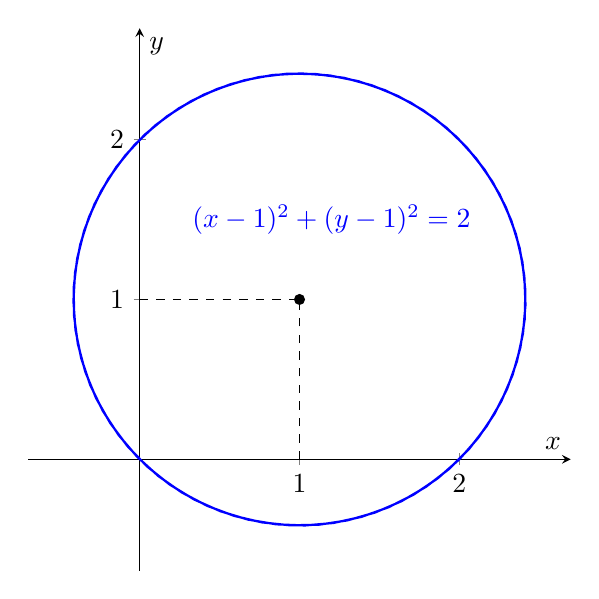
\begin{tikzpicture}
  \begin{axis}[
      axis lines = center,
      xlabel = {$x$},
      ylabel = {$y$},
      samples=100,
      xtick={1,2}, ytick={1,2},
      scale=1.21,
      axis equal image,
      enlargelimits=true,
    ]
    
    \addplot[blue, thick, domain=0:360] ({(2*sin(x)+2*cos(x))*cos(x)}, {(2*sin(x)+2*cos(x))*sin(x)});
    \fill (axis cs:1,1) circle (2pt);
    \node[blue] at (1.2,1.5) {$(x-1)^2+(y-1)^2=2$};
    \draw[dashed](1,0)--(1,1); \draw[dashed](0,1)--(1,1);
  \end{axis}
\end{tikzpicture}
\end{center}

\hfill

\noindent (ii) Rearrange the equation.

\[r=\tan\theta\sec\theta=\frac{\sin\theta}{\cos^2\theta}\implies r\cos^2\theta=\sin\theta\implies r^2\cos^2\theta=r\sin\theta\]

\hfill

\noindent Using the equations $x=r\cos\theta$ and $y=r\sin\theta$, we get the parabola $x^2=y$, where its branches open upward along the $y$-axis with the vertex $(0,0)$.

\begin{center}
\begin{tikzpicture}
  \begin{axis}[
      axis lines = center,
      xlabel = {$x$},
      ylabel = {$y$},
      samples=100,
      scale=1.21,
      axis equal image,
      enlargelimits=true,
    ]
    
    \addplot[blue, thick, domain=-2:2] {x^2};
    \node[blue] at (1.2,3) {$y=x^2$};
  \end{axis}
\end{tikzpicture}
\end{center}
\noindent 3.

\hfill

\noindent (a)

\hfill

\noindent (i) If $\mathbf u$ and $\mathbf v$ are perpendicular, the dot product of these vectors is equal to zero.

\[\mathbf u\cdot\mathbf v=\left\langle6,-3,2\right\rangle\cdot\left\langle4p+1,\,p-2,\,1\right\rangle=6(4p+1)-3(p-2)+2\cdot1=21p+14=0\implies p=\boxed{-\frac23}\]

\hfill

\noindent (ii) If $\mathbf u$ and $\mathbf v$ are parallel, the cross product of these vectors is equal to the zero vector.

\begin{align*}\mathbf{u}\times\mathbf{v}&=\left|\begin{array}{ccc}
\mathbf{i}&\mathbf{j}&\mathbf{k}\\
6&-3&2\\
4p+1&p-2&1
\end{array}\right|=\mathbf{i}\left|\begin{array}{cc}
-3&2\\p-2&1
\end{array}\right|-\mathbf{j}\left|\begin{array}{cc}
6&2\\4p+1&1
\end{array}\right|+\mathbf{k}\left|\begin{array}{cc}
6&-3\\4p+1&p-2
\end{array}\right|\\\\&=[1\cdot(-3)-2(p-2)]\mathbf i-(6\cdot1-2(4p+1))\mathbf j+[6(p-2)-(-3)(4p+1)]\mathbf k\\\\&=(1-2p)\mathbf i-(4-8p)\mathbf j+(-9+18p)\mathbf k=\mathbf0\implies \boxed{p=\frac12}\end{align*}

\hfill

\noindent (b) The sides of an equilateral triangle have the same length.

\[\overrightarrow{AB}=\left\langle3-5,\,1-1,\,5-3\right\rangle=\left\langle-2,0,2\right\rangle\rightarrow\left|\overrightarrow{AB}\right|=\sqrt{(-2)^2+0^2+2^2}=\sqrt8\]
\[\overrightarrow{AC}=\left\langle5-5,\,3-1,\,5-3\right\rangle=\left\langle0,2,2\right\rangle\rightarrow\left|\overrightarrow{AC}\right|=\sqrt{0^2+2^2+2^2}=\sqrt8\]
\[\overrightarrow{BC}=\left\langle5-3,\,3-1,\,5-5\right\rangle=\left\langle2,2,0\right\rangle\rightarrow\left|\overrightarrow{AC}\right|=\sqrt{2^2+2^2+0^2}=\sqrt8\]

\hfill

\noindent Half of the magnitude of the cross product of two vectors gives us the area of the triangle.

\[\frac12\left|\overrightarrow{AB}\times\overrightarrow{AC}\right|=\frac12\left|\overrightarrow{AB}\right|\left|\overrightarrow{AC}\right|\sin\frac\pi3=\frac12\cdot\sqrt8\cdot\sqrt8\cdot\frac{\sqrt3}2=\boxed{2\sqrt3}\]

\hfill

\noindent 4.

\hfill

\noindent (a) The planes have the same normal $\mathbf n=\left\langle1,1,1\right\rangle$. Using the definition $\mathbf n\cdot\overrightarrow{PP_0}=0$, we obtain

\[1(x-1)+1(y-2)+1(z-3)=0\implies\boxed{x+y+z=6}\]

\hfill

\noindent (b) The direction vector of the line is the normal vector of the plane. Therefore, the parametric equations for the line $L$ is as follows.

\[\boxed{\left.\begin{array}{l}
x=1+t\\
y=2+t\\
z=3+t
\end{array}\right\}\quad t\in\mathbb{R}}\]

\hfill

\noindent (c) Substitute the equation of $L$ in the equation of the plane $R$.

\[x+y+z=1\implies (1+t)+(2+t)+(3+t)=1\implies 3t+6=1\implies t=-\frac53\]
\[t=-\frac53\implies x=1-\frac53=-\frac23,\quad y=2-\frac53=\frac13,\quad z=3-\frac53=\frac43\]

\hfill

\noindent Therefore, the point of intersection is $\boxed{\left(-\frac23,\frac13,\frac43\right)}$.

\hfill

\noindent 5. 

\hfill

\noindent (a) Apply the Two-Path Test.

\[y=x\implies\lim_{(x,y)\to(0,0)}\frac{x^3y}{x^6+y^2}=\lim_{x\to0}\frac{x^4}{x^6+x^2}=\lim_{x\to0}\frac{x^2}{x^4+1}=\frac01=0\]
\[y=x^3\implies\lim_{(x,y)\to(0,0)}\frac{x^3y}{x^6+y^2}=\lim_{x\to0}\frac{x^6}{2x^6}=\lim_{x\to0}\frac12=\frac12\]

\hfill

\noindent Since $0\neq\dfrac12$, by the Two-Path Test, the limit does not exist.

\hfill

\noindent (b) We have the inequality $\left|\sin\theta\right|\leq1$ for all values of $\theta$. Therefore,

\[-1\leq\sin\left(\frac1{x^2+|y|}\right)\leq1\qquad\left[\text{except for }x=0,\,y=0\right]\]
\[-x^4\leq x^4\sin\left(\frac1{x^2+|y|}\right)\leq x^4\]

\[\lim_{(x,y)\to(0,0)}-x^4=\lim_{(x,y)\to(0,0)}x^4=0\implies\lim_{(x,y)\to(0,0)}x^4\sin\left(\frac1{x^2+|y|}\right)=\boxed0\]

\hfill

\noindent By the squeeze theorem, the limit is equal to zero.

\newpage

\noindent 6.

\hfill

\noindent (a) Parametrize the curve using $0\leq t\leq 2\pi$.

\[x=\cos t,\:y=\sin t,\:z=4\cos^2t,\qquad0\leq t\leq2\pi\]
\[\boxed{\mathbf r(t)=\left\langle\cos t,\,\sin t,\,4\cos^2t\right\rangle\qquad0\leq t\leq2\pi}\]

\hfill

\noindent (b) The tangent vector can be obtained by taking the first derivative of the vector function.

\[\mathbf T(t)=\mathbf r'(t)=\left\langle-\sin t,\,\cos t,\,-8\cos t\sin t\right\rangle\]

\hfill

\noindent The unit tangent vector is

\[\frac{\mathbf T(t)}{\left|\mathbf T(t)\right|}=\frac{\left\langle-\sin t,\,\cos t,\,-8\cos t\sin t\right\rangle}{\sqrt{(-\sin t)^2+(\cos t)^2+(-8\cos t\sin t)^2}}=\frac{\left\langle-\sin t,\,\cos t,\,-8\cos t\sin t\right\rangle}{\sqrt{1+64\cos^2t\sin^2t}}\]

\hfill

\noindent At $t=\dfrac\pi2$,

\[\frac{\mathbf T(t=\pi/2)}{|\mathbf T(t=\pi/2)|}=\frac{\left\langle-\sin\dfrac\pi2,\,\cos \dfrac\pi2,\,-8\cos\dfrac\pi2\sin\dfrac\pi2\right\rangle}{\sqrt{1+64\cos^2\dfrac\pi2\sin^2\dfrac\pi2}}=\boxed{\left\langle-1,0,0\right\rangle}\]

\hfill

\noindent (c) The length of the parametrized curve $\mathbf{r}(t)=\left\langle x(t),\,y(t),\,z(t)\right\rangle$ for $a\leq t\leq b$ can be evaluated using the integral

\[L=\int_a^b\left|\frac{d\mathbf r}{dt}\right|\,dt\]

\hfill

\noindent The length of the curve is then

\begin{align*}L&=\int_0^{2\pi}\left|\frac{d\mathbf r}{dt}\right|\,dt=\boxed{\int_0^{2\pi}\sqrt{1+64\cos^2t\sin^2t}\,dt=\int_0^{2\pi}\sqrt{1+16\sin^22t}\,dt}\end{align*}

\hfill

\noindent 7. This is a circular paraboloid with the vertex $(0,0,2)$ opening downward along the $z$-axis.

\begin{center}
\begin{tikzpicture}
  \begin{axis}[
  title={Plane $x=0$},
    xlabel=$y$, ylabel=$z$,
    xtick=\empty, ytick=\empty,
    samples=50,
    axis lines=middle,
    clip=true,
    scale=1,
    enlargelimits=true
    ]
    \addplot[domain=-5:5, blue] {-x^2/4+2};

    \node[blue] at (2.2,-2.8) {$z=-y^2+2$};
  \end{axis}
\end{tikzpicture}\hspace{1em}
\begin{tikzpicture}
  \begin{axis}[
  title={Plane $y=0$},
    xlabel=$x$, ylabel=$z$,
    xtick=\empty, ytick=\empty,
    samples=50,
    axis lines=middle,
    clip=true,
    scale=1,
    enlargelimits=true
    ]
    \addplot[domain=-5:5, red] {-x^2/4+2};

    \node[red] at (2.2,-2.8) {$z=-x^2+2$};
  \end{axis}
\end{tikzpicture}

\begin{tikzpicture}
  \begin{axis}[
  title={Plane $z=0$},
  axis equal image,
    xlabel=$x$, ylabel=$y$,
    xtick=\empty, ytick=\empty,
    samples=300,
    axis lines=middle,
    clip=true,
    scale=1,
    enlargelimits=true
    ]
    \addplot[domain=-sqrt(2):sqrt(2), orange] {sqrt(2-x^2)};
    \addplot[domain=-sqrt(2):sqrt(2), orange] {-sqrt(2-x^2)};

    \node[orange] at (0.7,0.2) {$x^2+y^2=2$};
  \end{axis}
\end{tikzpicture}\hspace{1em}
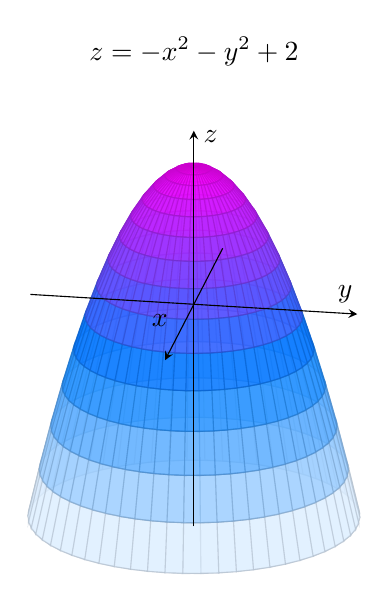
\begin{tikzpicture}
  \begin{axis}[
    title={$\displaystyle z=-x^2-y^2+2$},
    title style={yshift=-10pt},
      view={100}{20},
      axis lines=center,
      axis equal image,
      xlabel={$x$},
      ylabel={$y$},
      zlabel={$z$},
      domain=0:2*pi,
      y domain=-2.25:2.25,
      samples=30,
      samples y=30,
      colormap/cool,
      axis on top,
      scale=1.5,
      xtick=\empty, ytick=\empty, ztick=\empty,
      z buffer=sort,
      zmin=-3.2, zmax=2.5
    ]
    \addplot3[
      surf,
      opacity=0.6
    ]
    ({y*cos(deg(x))},
      {y*sin(deg(x))},
      {-y^2+2});
  \end{axis}
\end{tikzpicture}
\end{center}

\newpage

\vspace*{\fill}
\begin{center}
\Huge \textbf{FINAL SOLUTIONS}
\end{center}
\vspace*{\fill}
\newpage

\begin{center}
2019-2020 Spring Final (01/07/2020) Solutions\\
(Last update: 30/08/2025 02:16)
\end{center}

\noindent 1. Let $g(x,y,z)=x^2+y^2+z^2-100$ and then, solve the system of equations below using the method of Lagrange multipliers.

\[
\left.
\begin{array}{l}
\displaystyle\nabla f=\lambda\nabla g\\
\displaystyle g(x,y,z)=0
\end{array}
\right\}\quad\begin{array}{c}
\nabla f=\left\langle1,-1,1\right\rangle=\lambda\left\langle2x,2y,2z\right\rangle=\lambda\nabla g\\[1em]\displaystyle\therefore\: x=\frac1{2\lambda},\quad y=-\frac1{2\lambda},\quad z=\frac1{2\lambda}
\end{array}
\]

\hfill

\noindent Use the constraint.

\[g(x,y,z)=0\implies\left(\frac1{2\lambda}\right)^2+\left(-\frac1{2\lambda}\right)^2+\left(\frac1{2\lambda}\right)^2=100\implies\frac3{4\lambda^2}=100\implies\lambda=\pm\frac{\sqrt3}{20}\]

\[\lambda=\pm\frac{\sqrt3}{20\lambda}\implies x=\pm\frac{10\sqrt3}3,\quad y=\mp\frac{10\sqrt3}3,\quad z=\pm\frac{10\sqrt3}3\quad\]

\hfill

\noindent The absolute extrema occur at $\left(\frac{10\sqrt3}3,-\frac{10\sqrt3}3,\frac{10\sqrt3}3\right)$ and $\left(-\frac{10\sqrt3}3,\frac{10\sqrt3}3,-\frac{10\sqrt3}3\right)$.

\[f\left(\frac{10\sqrt3}3,-\frac{10\sqrt3}3,\frac{10\sqrt3}3\right)=10\sqrt3,\quad f\left(-\frac{10\sqrt3}3,\frac{10\sqrt3}3,-\frac{10\sqrt3}3\right)=-10\sqrt3\]

\[\boxed{\text{The minimum value is }{-10\sqrt3}\text{ and the maximum value is }10\sqrt3.}\]

\hfill

\noindent 2. Recall that 12 inches is 1 foot. The volume of a right circular cylinder is

\[V(r,h)=\pi r^2 h\]

\hfill

\noindent The total differential is

\[dV=V_r\,dr+V_h\,dh=\pi\left(2r\cdot h\right)\,dr+\pi\left(r^2\cdot 1\right)\,dh\]

\hfill

\noindent Set $r=1,\:h=4,\:dr=-0.2/12=-1/60,\:dh=-0.4/12=-1/30$.

\[dV=\pi\left(2\cdot1\cdot 4\right)\cdot\left(-\frac1{60}\right)+\pi\left(1^2\right)\left(-\frac1{30}\right)=-\frac\pi6\]

\hfill

\noindent Calculate the volume of the outer cylinder.

\[V(1,4)=\pi\cdot1^2\cdot4=4\pi\]

\hfill

\noindent Take $\displaystyle\Delta V\approx dV=-\frac\pi6$. Therefore, the volume of the interior can be approximated as follows.

\[\boxed{V\approx4\pi-\frac\pi6=\frac{23\pi}6}\]

\newpage

\noindent 3. We have $x=r\cos\theta$ and $y=r\sin\theta$. Compute the first-order partial derivatives.

\[\frac{\partial z}{\partial r}=\frac{\partial z}{\partial x}\cdot\frac{\partial x}{\partial r}+\frac{\partial z}{\partial y}\cdot\frac{\partial y}{\partial r},\qquad\frac{\partial z}{\partial \theta}=\frac{\partial z}{\partial x}\cdot\frac{\partial x}{\partial \theta}+\frac{\partial z}{\partial y}\cdot\frac{\partial y}{\partial \theta}\]

\hfill

\[\frac{\partial x}{\partial r}=\cos\theta,\qquad\frac{\partial y}{\partial r}=\sin\theta,\qquad\frac{\partial x}{\partial \theta}=-r\sin\theta,\qquad\frac{\partial y}{\partial\theta}=r\cos\theta,\]

\hfill

\noindent Rewrite $\displaystyle\frac{\partial z}{\partial r}$ and $\displaystyle\frac{\partial z}{\partial\theta}$.

\[\frac{\partial z}{\partial r}=\frac{\partial z}{\partial x}\cdot\cos\theta+\frac{\partial z}{\partial y}\cdot\sin\theta\]

\[\frac{\partial z}{\partial\theta}=\frac{\partial z}{\partial x}\cdot(-r\sin\theta)+\frac{\partial z}{\partial y}\cdot(r\cos\theta)\implies\frac1r\cdot\frac{\partial z}{\partial\theta}=\frac{\partial z}{\partial x}\cdot(-\sin\theta)+\frac{\partial z}{\partial y}\cdot\cos\theta\]

\hfill

\noindent Take the squares of both sides of the equations and add up side by side.

\[\left(\frac{\partial z}{\partial r}\right)^2=\left(\frac{\partial z}{\partial x}\cdot\cos\theta+\frac{\partial z}{\partial y}\cdot\sin\theta\right)^2,\quad\left(\frac1r\cdot\frac{\partial z}{\partial\theta}\right)^2=\left(\frac{\partial z}{\partial x}\cdot(-\sin\theta)+\frac{\partial z}{\partial y}\cdot\cos\theta\right)^2\]

\hfill

\begin{align*}
\left(\frac{\partial z}{\partial r}\right)^2+\frac1{r^2}\left(\frac{\partial z}{\partial\theta}\right)^2&=\left(\frac{\partial z}{\partial x}\right)^2\cos^2\theta+\frac{\partial z}{\partial x}\cdot\frac{\partial z}{\partial y}\cdot\cos\theta\sin\theta+\left(\frac{\partial z}{\partial y}\right)^2\sin^2\theta\\\\&\quad\:\;+\left(\frac{\partial z}{\partial x}\right)^2\sin^2\theta-\frac{\partial z}{\partial x}\cdot\frac{\partial z}{\partial y}\cdot\cos\theta\sin\theta+\left(\frac{\partial z}{\partial y}\right)^2\cos^2\theta
\end{align*}

\hfill

\noindent The terms with $\sin\theta\cos\theta$ cancel each other. Recall the equation $\displaystyle \sin^2x+\cos^2x=1$. The equation then becomes

\[\left(\frac{\partial z}{\partial r}\right)^2+\frac1{r^2}\left(\frac{\partial z}{\partial\theta}\right)^2=\left(\frac{\partial z}{\partial x}\right)^2+\left(\frac{\partial z}{\partial y}\right)^2,\]

\hfill

\noindent which we set out to demonstrate.

\hfill

\noindent 4.
\begin{center}
\begin{minipage}{0.5\textwidth}
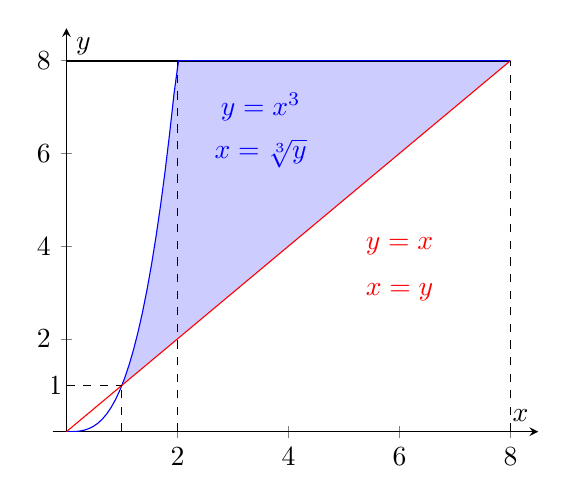
\begin{tikzpicture}
  \begin{axis}[
      axis lines = middle,
      xlabel = $x$, ylabel = $y$,
      domain=0:8,
      ymin=0, ymax=8.7,
      xmin=-0.25, xmax=8.5,
      samples=100,
      clip=true,
      scale=0.9,
    ]
    
    \addplot [name path=A, domain=1:8, draw=none] {x};
    \addplot [name path=B, domain=1:8, draw=none] {min(x^3,8)};
    \addplot [fill=blue!20, draw=none] fill between [of=A and B, soft clip={domain=1:8}];

    \node at (-0.2,1) {$1$};
    \draw[thick] (0,8)--(8,8);
    \addplot [blue, domain=0:8] {min(x^3,8)};
    \addplot [red, domain=0:8] {x};
    \draw[dashed] (1,0)--(1,1); \draw[dashed] (0,1)--(1,1); \draw[dashed] (2,0)--(2,8); \draw[dashed] (8,0)--(8,8);

    \node[red] at (6,4) {$y=x$}; \node[red] at (6,3) {$x=y$};
    \node[blue] at (3.5,7) {$y=x^3$}; \node[blue] at (3.5,6) {$x=\sqrt[3]{y}$};
  \end{axis}
\end{tikzpicture}
\end{minipage}\begin{minipage}{0.45\textwidth}
\[\boxed{\int_1^8\int_{\sqrt[3]y}^yf(x,y)\,dx\,dy}\]
\end{minipage}
\end{center}

\newpage

\hfill

\noindent 5. 
\begin{align*}\int_1^2\int_{y^2}^{y^5}\mathrm{e}^{x/y^2}\,dx\,dy&=\int_1^2\left[y^2\cdot{\mathrm{e}^{x/y^2}}\right]_{x=y^2}^{x=y^5}\,dy=\int_1^2\left(y^2\cdot\mathrm{e}^{y^3}-y^2\cdot\mathrm{e}\right)\,dy=\left[\frac13\mathrm{e}^{y^3}-\frac13\mathrm{e}y^3\right]_1^2\\\\&=\frac13\mathrm{e}^{8}-\frac{8\mathrm{e}}3-\left(\frac13\mathrm{e}^1-\frac13\mathrm{e}\right)=\boxed{\frac{\mathrm{e}}3\left(\mathrm{e}^7-8\right)}\end{align*}

\hfill

\noindent 6.
\begin{center}
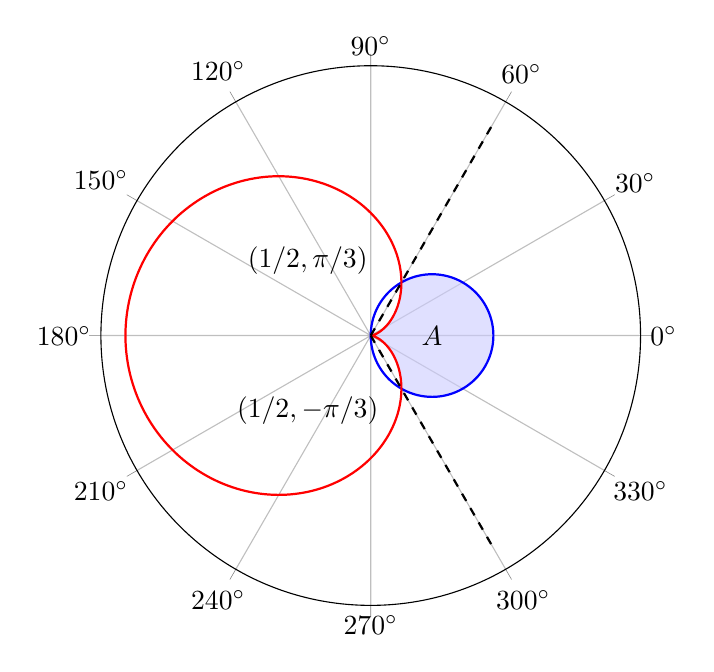
\begin{tikzpicture}
  \begin{polaraxis}[ytick=\empty, axis y line=none, xticklabel=$\pgfmathprintnumber{\tick}^\circ$,]
    \addplot [
      domain=-pi/3:pi/3,
      samples=300,
      draw=none,
      name path=A,
      data cs=polarrad,
    ] {cos(deg(x))};

    \addplot [
      domain=-pi/3:pi/3,
      samples=300,
      draw=none,
      name path=B,
      data cs=polarrad,
    ] {1-cos(deg(x))};

    \addplot [
      blue!20,
      fill opacity=0.6,
    ] fill between[of=A and B];

    \addplot [
      domain=0:2*pi,
      samples=300,
      thick,
      blue,
      data cs=polarrad,
    ] {cos(deg(x))};

    \addplot [
      domain=0:2*pi,
      samples=300,
      thick,
      red,
      data cs=polarrad,
    ] {1-cos(deg(x))};

    \draw[black, thick, dashed] (axis cs: 60,0) -- (axis cs: 60,2);
    \draw[black, thick, dashed] (axis cs: -60,0) -- (axis cs: -60,2);

    \node at (axis cs:130,0.8) {$(1/2,\pi/3)$};
    \node at (axis cs:-130,0.8) {$(1/2,-\pi/3)$};
    \node at (0,0.5) {$A$};

  \end{polaraxis}
\end{tikzpicture}
\end{center}

\begin{align*}
A&=\int_{-\pi/3}^{\pi/3}\int_{1-\cos\theta}^{\cos\theta}\,r\,dr\,d\theta=\frac12\int_{-\pi/3}^{\pi/3}\left[\cos^2\theta-(1-\cos\theta)^2\right]\,d\theta=\frac12\int_{-\pi/3}^{\pi/3}\left(2\cos\theta-1\right)\,d\theta\\\\&=\frac12\bigg[2\sin\theta-\theta\bigg]_{-\pi/3}^{\pi/3}=\frac12\left[\left(2\sin\frac\pi3-\frac\pi3\right)-\left(2\sin\left(-\frac\pi3\right)+\frac\pi3\right)\right]=\boxed{\sqrt3-\frac\pi3}
\end{align*}

\hfill

\noindent 7. For cylindrical coordinates, we have

\[
\begin{array}{c}
z=z\\
r^2=x^2+y^2\\
dV=r\,dz\,dr\,d\theta
\end{array}\quad\rightarrow\quad
\begin{array}{c}
\displaystyle z=\sqrt{x^2+y^2}\implies z=\sqrt{r^2}\implies z_{\text{lower}}=r\\[1em]
z=2-x^2-y^2\implies z_{\text{upper}}=2-r^2\\[1em]
0\leq\theta\leq2\pi
\end{array}
\]

\hfill

\noindent Find where the surfaces $z=r$ and $z=2-r^2$ intersect to determine the upper bound of $r$.

\begin{align*}\left.\begin{array}{c}
z=r\\
z=2-r^2
\end{array}\right\}\quad r^2+r-2=0\implies (r+2)(r-1)=0\implies r_{\text{upper}}=1\end{align*}

\newpage

\begin{align*}\mathrm{I}&=\int_0^{2\pi}\int_0^1\int_{r}^{2-r^2}r\,dz\,dr\,d\theta=\int_0^{2\pi}\int_0^1\bigg[z\bigg]_{z=r}^{z=2-r^2}r\,dr\,d\theta=\int_0^{2\pi}\int_0^1\left(2-r^2-r\right)\,r\,dr\,d\theta\\\\&=\int_0^{2\pi}\int_0^1\left(2r-r^3-r^2\right)\,dr\,d\theta=\int_0^{2\pi}\left[r^2-\frac{r^4}4-\frac{r^3}3\right]_{r=0}^{r=1}\,d\theta=\int_0^{2\pi}\frac5{12}\,d\theta=\frac5{12}\cdot\theta\,\bigg|_0^{2\pi}\\\\&=\boxed{\frac{5\pi}6}\end{align*}

\hfill

\noindent 8. For spherical coordinates, we have

\[
\left.\begin{array}{c}
z=\rho\cos\phi\\
r=\rho\sin\phi\\
x^2+y^2+z^2=\rho^2\\
dV=\rho^2\sin\phi\,d\rho\,d\phi\,d\theta
\end{array}\right.\begin{array}{c}
x^2+y^2+z^2=7\implies\rho^2=7\implies\rho_{\text{upper},1}=\sqrt7\\
z=x^2+y^2\implies\rho\cos\phi=\rho^2\sin^2\phi\implies\rho_{\text{upper},2}=\cot\phi\csc\phi\\[1em]
\sin\left(\sqrt{x^2+y^2+z^2}\right)=\sin\left(\sqrt{\rho^2}\right)=\sin\rho\\[1em]
\displaystyle0\leq\theta\leq\frac\pi2
\end{array}\]

\hfill

\noindent Find where the surfaces $z=x^2+y^2$ and $x^2+y^2+z^2=7$ intersect to find the bounds of $\phi$.

\[\begin{array}{c}\displaystyle z^2+z-7=0\implies z_{1,2}=\frac{-1\pm\sqrt{1^2-4\cdot1\cdot(-7)}}2\\[1em]\displaystyle z>0\implies z=\rho\cos\phi=\sqrt7\cos\phi=\frac{-1+\sqrt{29}}{2}\\[1em]\displaystyle\cos\phi=\frac{-1+\sqrt{29}}{2\sqrt7}\implies\phi=\arccos\left(\frac{-1+\sqrt{29}}{2\sqrt7}\right)\end{array}\]

\hfill

\noindent For $\displaystyle\phi<\arccos\left(\frac{-1+\sqrt{29}}{2\sqrt7}\right)$, the upper bound for $\rho$ is $\sqrt7$. For $\displaystyle\phi>\arccos\left(\frac{-1+\sqrt{29}}{2\sqrt7}\right)$, the lower bound is $\cot\phi\csc\phi$.

\[\boxed{\begin{array}{l}\displaystyle\int_0^{\pi/2}\int_0^{\arccos\left(\textstyle\frac{-1+\sqrt{29}}{2\sqrt7}\right)}\int_0^{\sqrt7}\sin\rho \cdot\rho^2\sin\phi\,d\rho\,d\phi\,d\theta\\\\\displaystyle+\int_0^{\pi/2}\int_{\arccos\left(\textstyle\frac{-1+\sqrt{29}}{2\sqrt7}\right)}^{\pi/2}\int_0^{\cot\phi\csc\phi}\sin\rho\cdot\rho^2\sin\phi\,d\rho\,d\phi\,d\theta\end{array}}\]

\hfill

\noindent Since we choose the minimum of the upper bounds of $\rho$, we can write the equivalent expression.

\[\boxed{\int_0^{\pi/2}\int_0^{\pi/2}\int_0^{\min\left(\sqrt7,\cot\phi\csc\phi\right)}\sin\rho\cdot\rho^2\sin\phi\,d\rho\,d\phi\,d\theta}\]

\newpage


\begin{center}
2019-2020 Spring Resit (01/07/2020) Solutions\\
(Last update: 08/08/2025 22:44)
\end{center}

\noindent 1. Let $g(x,y,z)=x+y+z-10$ and then, solve the system of equations below using the method of Lagrange multipliers.

\[
\left.
\begin{array}{ll}
\displaystyle\nabla T =\lambda \nabla g\\
\displaystyle g(x,y,z) = 0
\end{array}
\right\}\quad
\nabla T = \left\langle-y-z,-x-z,-x-y\right\rangle=\lambda\left\langle1,1,1\right\rangle= \lambda\nabla g
\]

\begin{align*}T_x+T_y + T_z&=(-y-z) +(-x-z) +(-x-y)=-2x-2y-2z\\&=\lambda+\lambda+\lambda=3\lambda\implies x+y+z=\frac{-3\lambda}{2}\end{align*}

\hfill

\noindent Use the constraint to find the value of $\lambda$.

\[g(x,y,z) = 0 \implies \frac{-3\lambda}{2}-10=0\implies \lambda=-\frac{20}{3}\]

\hfill

\noindent So far, we have the equations below. Solve the system of equations and find the values of $x,y,z$ one by one.

\[
\left.
\begin{array}{ll}
\displaystyle -y-z=-\frac{20}{3}&(1)\\[0.5cm]
\displaystyle -x-z=-\frac{20}{3}&(2)\\[0.5cm]
\displaystyle -x-y=-\frac{20}{3}&(3)
\end{array}
\right\}\quad
\begin{array}{ll}
\displaystyle (1)\:\&\:(2)\rightarrow x-y=0 & (4) \\[0.2cm]
\displaystyle (3)\:\&\:(4)\rightarrow y=\frac{10}{3}&(5)\\[0.5cm]
\displaystyle\therefore z=\frac{10}{3},\quad x=\frac{10}{3}
\end{array}
\]

\hfill

\noindent We now have all the values. Substitute in $T(x,y,z)$ to find the minimum value of the temperature.

\[T_{\text{min}}=T\left(\frac{10}{3},\frac{10}{3},\frac{10}{3}\right)=100-\left(\frac{10}{3}\right)^2-\left(\frac{10}{3}\right)^2-\left(\frac{10}{3}\right)^2=\boxed{\frac{200}{3}}\]

\hfill

\noindent 2. We have $x=r\cos\theta$ and $y=r\sin\theta$.

\[x^2=r^2\cos^2\theta,\quad y^2 =r^2\sin^2\theta\implies x^2+y^2=r^2\left(\cos^2\theta+\sin^2\theta\right)=r^2, \quad \therefore  r=\sqrt{x^2+y^2}\]

\[\frac{y}{x}=\frac{r\sin\theta}{r\cos\theta}=\tan\theta \implies \theta=\tan^{-1}\frac{y}{x}\]

\hfill

\noindent Compute the first-order partial derivatives.

\[\frac{\partial z}{\partial x}=\frac{\partial z}{\partial r}\cdot\frac{\partial r}{\partial x}+\frac{\partial z}{\partial \theta}\cdot\frac{\partial\theta}{\partial x},\quad\quad\frac{\partial z}{\partial y}=\frac{\partial z}{\partial r}\cdot\frac{\partial r}{\partial y} + \frac{\partial z}{\partial\theta}\cdot\frac{\partial\theta}{\partial y}\]

\hfill

\[\frac{\partial r}{\partial x}=\frac{x}{\sqrt{x^2+y^2}}=\cos\theta,\quad\quad\frac{\partial r}{\partial y}=\frac{y}{\sqrt{x^2+y^2}}=\sin\theta\]

\newpage

\[\quad\frac{\partial\theta}{\partial x}=\frac{1}{\displaystyle 1+\frac{y^2}{x^2}}\cdot \left(-\frac{y}{x^2}\right)=\frac{-y}{x^2+y^2}=\frac{-\sin\theta}{r},\quad\quad\frac{\partial\theta}{\partial y}=\frac{1}{\displaystyle1+\frac{y^2}{x^2}}\cdot\frac{1}{x}=\frac{x}{x^2+y^2}=\frac{\cos\theta}{r}\]

\hfill

\noindent Rewrite $\displaystyle\frac{\partial z}{\partial x}$ and $\displaystyle\frac{\partial z}{\partial y}$.

\[\frac{\partial z}{\partial x}=\frac{\partial z}{\partial r}\cdot\frac{x}{\sqrt{x^2+y^2}}+\frac{\partial z}{\partial\theta}\cdot\frac{-y}{x^2+y^2},\quad\quad\frac{\partial z}{\partial y}=\frac{\partial z}{\partial r}\cdot\frac{y}{\sqrt{x^2+y^2}}+\frac{\partial z}{\partial \theta}\cdot\frac{x}{x^2+y^2}\]

\hfill

\noindent Compute the second-order partial derivatives.

\[\frac{\partial}{\partial x}\left(\frac{\partial z}{\partial x}\right)=\frac{\partial}{\partial x}\left(\frac{\partial z}{\partial r}\cdot\frac{x}{\sqrt{x^2+y^2}}+\frac{\partial z}{\partial\theta}\cdot\frac{-y}{x^2+y^2}\right)\]

\begin{align*}\frac{\partial^2z}{\partial x^2}=&\left[\left(\frac{\partial^2z}{\partial r^2}\cdot\frac{\partial r}{\partial x}+\frac{\partial^2 z}{\partial\theta\,\partial r}\cdot\frac{\partial\theta}{\partial x}\right)\cdot\frac{x}{\sqrt{x^2+y^2}}+\frac{\partial z}{\partial r}\cdot\frac{1\cdot\sqrt{x^2+y^2}-x\cdot\frac{x}{\sqrt{x^2+y^2}}}{\left(\sqrt{x^2+y^2}\right)^2}\right]\\&+\left[\left(\frac{\partial^2z}{\partial \theta^2}\cdot\frac{\partial \theta}{\partial x}+\frac{\partial^2 z}{\partial r\,\partial \theta}\cdot\frac{\partial r}{\partial x}\right)\cdot\frac{-y}{x^2+y^2}+\frac{\partial z}{\partial\theta}\cdot\frac{y}{(x^2+y^2)^2}\cdot2x\right]\end{align*}

\hfill

\[\frac{\partial}{\partial y}\left(\frac{\partial z}{\partial y}\right)=\frac{\partial}{\partial y}\left(\frac{\partial z}{\partial r}\cdot\frac{y}{\sqrt{x^2+y^2}}+\frac{\partial z}{\partial \theta}\cdot\frac{x}{x^2+y^2}\right)\]

\begin{align*}\frac{\partial^2z}{\partial y^2}=&\left[\left(\frac{\partial^2z}{\partial r^2}\cdot\frac{\partial r}{\partial y}+\frac{\partial^2 z}{\partial\theta\,\partial r}\cdot\frac{\partial\theta}{\partial y}\right)\cdot\frac{y}{\sqrt{x^2+y^2}}+\frac{\partial z}{\partial r}\cdot\frac{1\cdot\sqrt{x^2+y^2}-y\cdot\frac{y}{\sqrt{x^2+y^2}}}{\left(\sqrt{x^2+y^2}\right)^2}\right]\\&+\left[\left(\frac{\partial^2z}{\partial \theta^2}\cdot\frac{\partial \theta}{\partial y}+\frac{\partial^2 z}{\partial r\,\partial \theta}\cdot\frac{\partial r}{\partial y}\right)\cdot\frac{x}{x^2+y^2}+\frac{\partial z}{\partial\theta}\cdot\frac{-x}{(x^2+y^2)^2}\cdot2y\right]\end{align*}

\hfill

\noindent Add the second-order partial derivatives and set to $0$. The last terms eliminate each other. Write $x$ and $y$ in terms of $r$ and $\theta$.

\begin{align*}\frac{\partial^2 z}{\partial x^2}+\frac{\partial^2 z}{\partial y^2}=&\left[\left(\frac{\partial^2z}{\partial r^2}\cdot\cos\theta +\frac{\partial^2z}{\partial\theta\,\partial r}\cdot\frac{-\sin\theta}{r}\right)\cdot\cos\theta+\frac{\partial z}{\partial r}\cdot\frac{\sin^2\theta}{r}\right]\\\\&+\left[\left(\frac{\partial^2z}{\partial\theta^2}\cdot\frac{-\sin\theta}{r} + \frac{\partial^2z}{\partial r\,\partial\theta}\cdot\cos\theta\right)\cdot\frac{-\sin\theta}{r}\right]\\\\&+\left[\left(\frac{\partial^2z}{\partial r^2}\cdot\sin\theta +\frac{\partial^2z}{\partial\theta\,\partial r}\cdot\frac{\cos\theta}{r}\right)\cdot\sin\theta+\frac{\partial z}{\partial r}\cdot\frac{\cos^2\theta}{r}\right]\\\\&+\left[\left(\frac{\partial^2z}{\partial\theta^2}\cdot\frac{\cos\theta}{r} + \frac{\partial^2z}{\partial r\,\partial\theta}\cdot\sin\theta\right)\cdot\frac{\cos\theta}{r}\right]=0\end{align*}

\newpage

\noindent Inspect the terms that add up to $0$. Recall $\sin^2\theta+\cos^2\theta=1$, then the equation reduces to

\begin{align*}
\frac{\partial^2z}{\partial x^2}+\frac{\partial^2z}{\partial y^2}&=\frac{\partial^2z}{\partial r^2}\cdot\left(\cos^2\theta+\sin^2\theta\right)+\frac{\partial z}{\partial r}\cdot\frac{\sin^2\theta+\cos^2\theta}{r}+\frac{\partial^2z}{\partial\theta^2}\cdot\left(\sin^2\theta+\cos^2\theta\right)\\\\&=\frac{\partial^2z}{\partial r^2}+\frac1r\cdot\frac{\partial z}{\partial r}+\frac{\partial^2z}{\partial\theta^2}=0,
\end{align*}

\hfill

\noindent which we set out to demonstrate.

\hfill

\noindent 3. Change the order of integration using the graph below and then evaluate the integral.

\begin{center}
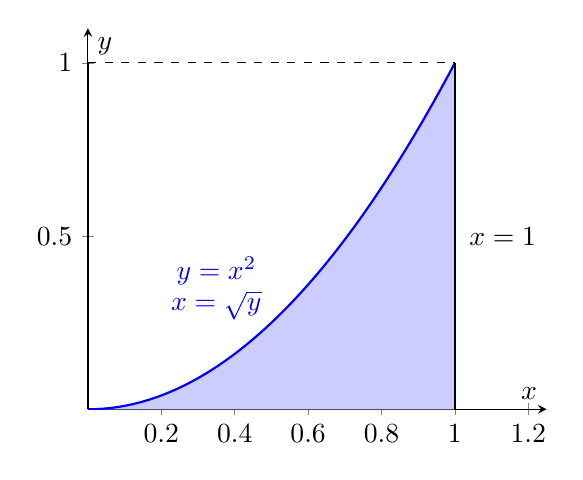
\begin{tikzpicture}
  \begin{axis}[
      axis lines = middle,
      xlabel = $x$, ylabel = $y$,
      domain=0:1,
      ymin=0, ymax=1.1,
      xmin=0, xmax=1.25,
      samples=100,
      clip=true,
      scale=0.85
    ]
    
    \addplot [
      name path=A,
      domain=0:1,
      draw=none,
    ] {x^2};

    \path[name path=B] (axis cs:0,1) -- (axis cs:1,1);
    \path[name path=C] (axis cs:0,0) -- (axis cs:0,1);
    \path[name path=D] (axis cs:0,0) -- (axis cs:1,0);

    \addplot [
      fill=blue!20,
      draw=none,
    ] fill between [
      of=A and D,
      soft clip={domain=0:1},
    ];
    
    \addplot[blue, thick] {x^2};
    \addplot[black, thick] coordinates {(0,0) (0,1)};
    \addplot[black, thick] coordinates {(1,0) (1,1)};
    \draw[dashed] (axis cs: 0,1) -- (axis cs: 1,1);
    \node at (axis cs: 1.13, 0.5) {$x=1$};
    \node[blue] at (axis cs: 0.35, 0.4) {$y=x^2$};
    \node[blue] at (axis cs: 0.35, 0.3) {$x=\sqrt{y}$};

  \end{axis}
\end{tikzpicture}
\end{center}
\begin{align*}
\int_0^1\int_{\sqrt{y}}^1\sqrt{1-x^3}\,dx\,dy&=\int_0^1\int_0^{x^2}\sqrt{1-x^3}\,dy\,dx=\int_0^1x^2\sqrt{1-x^3}\,dx\:\left[\begin{array}{c}u=1-x^3 \\du=-3x^2\,dx\end{array}\right]\\\\&=\int\frac{\sqrt{u}}{-3}\,du=-\frac29u^{3/2}+c=-\frac29\left(1-x^3\right)^{3/2}\Bigg|_0^1=0-\left[-\frac29\right]=\boxed{\frac29}\end{align*}

\hfill

\noindent 4.

\begin{minipage}{0.45\textwidth}
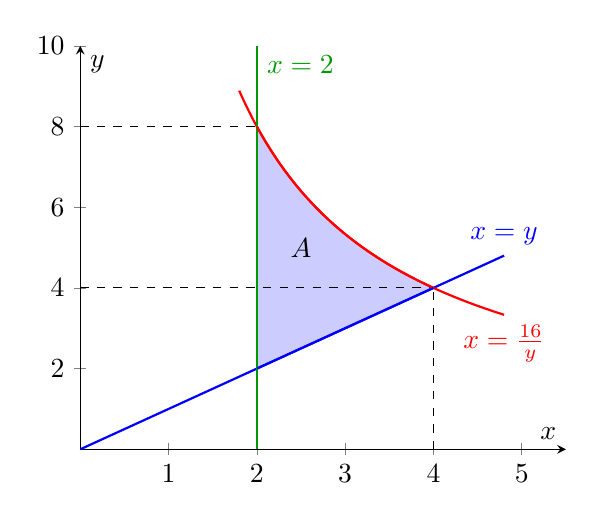
\begin{tikzpicture}
  \begin{axis}[
      axis lines = center,
      xlabel = {$x$},
      ylabel = {$y$},
      domain=1:4,
      samples=200,
      ymin=0, ymax=10,
      xmin=0, xmax=5.5,
      clip=true,
      scale=0.9
    ]
    
    \draw[dashed] (axis cs: 0,4) -- (axis cs: 4,4);
    \draw[dashed] (axis cs: 4,0) -- (axis cs: 4,4);
    \draw[dashed] (axis cs: 0,8) -- (axis cs:2,8);
    \node at (2.5,5) {$A$};

    \addplot[blue, thick, domain=0:4.8] {x} node[above] {$x = y$};

    \addplot[red, thick, domain=1.8:4.8] {16/x} node[below] {$x = \frac{16}{y}$};

    \addplot[green!60!black, thick, domain=0:10] ({2},x) node[below right] {$x = 2$};
    
    \addplot[red, thick, domain=2:4, name path=A] {16/x};
    \addplot[blue, thick, domain=2:4, name path=B] {x};

    \addplot [
      fill=blue!20,
      draw=none,
    ] fill between [
      of=A and B,
      soft clip={domain=2:4},
    ];
  \end{axis}
\end{tikzpicture}
\end{minipage}\hspace{0.25em}
\begin{minipage}{0.5\textwidth}
\begin{align*}A&=\int_2^4\int_2^y\,dx\,dy + \int_4^8\int_2^{16/y}\,dx\,dy\\\\&=\int_2^4\int_{x}^{\frac{16}x}\,dy\,dx=\int_2^4\left(\frac{16}x-x\right)\,dx\\\\&=\left[16\ln|x| -\frac{x^2}2\right]_2^4\\\\&=\left[\left(16\ln4 -\frac{4^2}{2}\right)-\left(16\ln2-\frac{2^2}{2}\right)\right]\\\\&=\boxed{16\ln2-6}\end{align*}
\end{minipage}

\newpage

\noindent 5.
\begin{center}
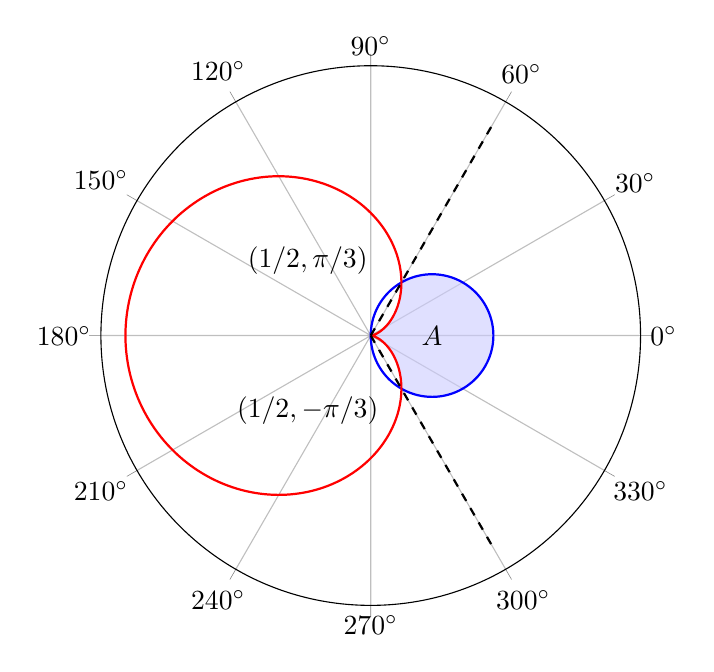
\begin{tikzpicture}
  \begin{polaraxis}[ytick=\empty, axis y line=none, xticklabel=$\pgfmathprintnumber{\tick}^\circ$,]
    \addplot [
      domain=-pi/3:pi/3,
      samples=300,
      draw=none,
      name path=A,
      data cs=polarrad,
    ] {cos(deg(x))};

    \addplot [
      domain=-pi/3:pi/3,
      samples=300,
      draw=none,
      name path=B,
      data cs=polarrad,
    ] {1-cos(deg(x))};

    \addplot [
      blue!20,
      fill opacity=0.6,
    ] fill between[of=A and B];

    \addplot [
      domain=0:2*pi,
      samples=300,
      thick,
      blue,
      data cs=polarrad,
    ] {cos(deg(x))};

    \addplot [
      domain=0:2*pi,
      samples=300,
      thick,
      red,
      data cs=polarrad,
    ] {1-cos(deg(x))};

    \draw[black, thick, dashed] (axis cs: 60,0) -- (axis cs: 60,2);
    \draw[black, thick, dashed] (axis cs: -60,0) -- (axis cs: -60,2);

    \node at (axis cs:130,0.8) {$(1/2,\pi/3)$};
    \node at (axis cs:-130,0.8) {$(1/2,-\pi/3)$};
    \node at (0,0.5) {$A$};

  \end{polaraxis}
\end{tikzpicture}
\end{center}

\begin{align*}
A&=\int_{-\pi/3}^{\pi/3}\int_{1-\cos\theta}^{\cos\theta}\,r\,dr\,d\theta=\frac12\int_{-\pi/3}^{\pi/3}\left[\cos^2\theta-(1-\cos\theta)^2\right]\,d\theta=\frac12\int_{-\pi/3}^{\pi/3}\left(2\cos\theta-1\right)\,d\theta\\\\&=\frac12\bigg[2\sin\theta-\theta\bigg]_{-\pi/3}^{\pi/3}=\frac12\left[\left(2\sin\frac\pi3-\frac\pi3\right)-\left(2\sin\left(-\frac\pi3\right)+\frac\pi3\right)\right]=\boxed{\sqrt3-\frac\pi3}
\end{align*}

\hfill

\noindent 6.
\begin{center}
    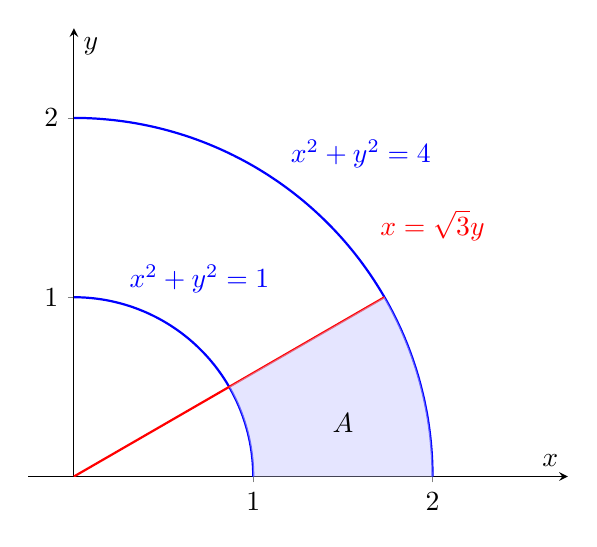
\begin{tikzpicture}
    \begin{axis}[
        axis equal,
        axis lines = center,
        xlabel = $x$,
        ylabel = $y$,
        xmin = 0, xmax = 2.5,
        ymin = 0, ymax = 2.5,
        xtick = {-2,-1,1,2},
        ytick = {-2,-1,1,2},
    ]

    \addplot[domain=0:90, samples=100, blue, thick] ({cos(x)}, {sin(x)});
    \addplot[domain=0:90, samples=100, blue, thick] ({2*cos(x)}, {2*sin(x)});
    \addplot[domain=0:1, red, thick] ({sqrt(3)*x}, {x});
    \fill[blue!20, opacity=0.5] 
        plot[domain=0:30, samples=30,variable=\t] ({2*cos(\t)}, {2*sin(\t)}) -- 
        plot[domain=30:0, samples=30,variable=\t] ({cos(\t)}, {sin(\t)}) -- cycle;
    \node[blue] at (1.6,1.8) {$x^2 + y^2 = 4$};
    \node[blue] at (0.7,1.1) {$x^2 + y^2 = 1$};
    \node[red] at (2,1.4) {$x = \sqrt{3}y$};
    \node at (1.5,0.3) {$A$};

    \end{axis}
\end{tikzpicture}
\end{center}

\noindent Use the following transformation to switch to polar coordinates.

\[
\begin{array}{c}x=r\cos\theta\\y=r\sin\theta\\[0.2cm]x^2+y^2=r^2\\[0.2cm]\displaystyle\theta=\tan^{-1}\frac yx\\[0.2cm]dA=r\,dr\,d\theta
\end{array}\quad\rightarrow\quad
\begin{array}{c}
x^2+y^2=1\,\implies\,r^2=1\implies r=1\\x^2+y^2=4\,\implies\,r^2=4\implies r=2\\y=0\implies\theta=0\\
\displaystyle x=\sqrt3y\implies\tan^{-1}\frac yx=\tan^{-1}\frac1{\sqrt3}\implies\theta=\frac{\pi}6\\\\\displaystyle\therefore 1\leq r\leq2,\quad 0\leq\theta\leq\frac{\pi}6
\end{array}
\]

\newpage

\begin{align*}
\int_0^{\pi/6}\int_1^2\sin(r^2)\,r\,dr\,d\theta&=\int_0^{\pi/6}\left[-\frac12\cos{r^2}\right]_1^2\,d\theta=-\frac12\int_0^{\pi/6}\left(\cos4-\cos1\right)\,d\theta\\\\&=\frac12(\cos1-\cos4)\cdot\theta\,\bigg|_0^{\pi/6}=\boxed{\frac\pi{12}(\cos1-\cos4)}
\end{align*}

\hfill

\noindent 7. For cylindrical coordinates, we have

\[
\begin{array}{c}
z=z\\
r^2=x^2+y^2\\
dV=r\,dz\,dr\,d\theta
\end{array}\quad\rightarrow\quad
\begin{array}{c}
\displaystyle2z=x^2+y^2\,\rightarrow\,z=\frac{r^2}2\\[0.3cm]
x^2+y^2+z^2=8\,\rightarrow\,z=\sqrt{8-r^2}\\
\end{array}
\]

\hfill

\noindent Find where the surfaces $2z=x^2+y^2$ and $x^2+y^2+z^2=8$ intersect to determine the limits of $r$.

\begin{align*}x^2+y^2+z^2=8&\implies 2z + z^2 = 8\implies (z+4)(z-2) = 0\implies z=2\\&\implies4=x^2+y^2=r^2 \implies r=2\end{align*}

\hfill

\noindent The lower limit of $r$ is apparently $0$. The region in the $xy$-plane is circular if we project the domain. Therefore, $0\leq\theta\leq2\pi$. Now, set up the triple integral in polar coordinates.

\begin{align*}\mathrm{I}&=\iiint_D\frac{dV}{x^2+y^2+z^2}=\int_0^{2\pi}\int_0^2\int_{r^2/2}^{\sqrt{8-r^2}}\frac{r}{r^2+z^2}\,dz\,dr\,d\theta\\\\&=\int_0^{2\pi}\int_0^2\int_{r^2/2}^{\sqrt{8-r^2}}\frac{1}{1+\left(\frac zr\right)^2}\cdot\frac1r\,dz\,dr\,d\theta=\int_0^{2\pi}\int_0^2\left[\arctan\left(\frac zr\right)\right]_{r^2/2}^{z=\sqrt{8-r^2}}\,dr\,d\theta\\\\&=\int_0^{2\pi}\int_0^2\arctan\left(\frac{\sqrt{8-r^2}}r\right)\,dr\,d\theta-\int_0^{2\pi}\int_0^2\arctan\left(\frac r2\right)\,dr\,d\theta\end{align*}

\hfill

\noindent $\theta$ is independent of $r$. Therefore, we can write the following.

\begin{equation}
\mathrm{I}=2\pi\int_0^2\arctan\left(\frac{\sqrt{8-r^2}}r\right)\,dr-2\pi\int_0^2\arctan\left(\frac r2\right)\,dr
\end{equation}

\hfill

\noindent Now, use integration by parts for the left-hand integral in $(1)$. Apply the chain rule and the quotient rule rigorously.

\begin{align*}
\displaystyle u=\arctan\left(\frac{\sqrt{8-r^2}}r\right)&\rightarrow\displaystyle du=\frac1{\displaystyle1+\left(\frac{\sqrt{8-r^2}}r\right)^2}\cdot\frac{\displaystyle \frac{1}{2\sqrt{8-r^2}}\cdot(-2r)\cdot r -\sqrt{8-r^2}\cdot 1}{r^2}\,dr\\
\displaystyle dv=dr&\rightarrow v=r
\end{align*}

\newpage

\noindent Notice that we have an improper integral, where we need to use limits.

\begin{align}
\int_0^2\arctan\left(\frac{\sqrt{8-r^2}}r\right)\,dr&=\lim_{T\to0^+}\left[r\cdot\arctan\left(\frac{\sqrt{8-r^2}}r\right)\Bigg|_T^2-\int_T^2r\cdot\frac{-1}{\sqrt{8-r^2}}\,dr\right]\nonumber\\\nonumber\\&=\lim_{T\to0^+}\left[r\cdot\arctan\left(\frac{\sqrt{8-r^2}}r\right)-\sqrt{8-r^2}\right]_T^2
\end{align}

\hfill

\noindent Compute the other integral in $(1)$ using integration by parts.

\begin{align*}
\displaystyle u=\arctan\left(\frac{r}2\right)&\rightarrow\displaystyle du=\frac1{\displaystyle1+\left(\frac{r}2\right)^2}\cdot\frac12\,dr\\
\displaystyle dv=dr&\rightarrow v=r
\end{align*}
\begin{align}
\int_0^2\arctan\left(\frac r2\right)\,dr&=r\cdot\arctan\left(\frac r2\right)\Bigg|_0^2-\int_0^2r\cdot\frac2{4+r^2}\,dr\nonumber\\\nonumber\\&=\left[r\cdot\arctan\left(\frac r 2\right)-\ln\left|4+r^2\right|\right]_0^2
\end{align}

\hfill

\noindent Rewrite $(1)$ using $(2)$ and $(3)$.

\begin{equation*}
\mathrm{I}=2\pi\lim_{T\to0^+}\left[r\cdot\arctan\left(\frac{\sqrt{8-r^2}}r\right)-\sqrt{8-r^2}\right]_T^2-2\pi\left[r\cdot\arctan\left(\frac r2\right)-\ln\left|4+r^2\right|\right]_0^2
\end{equation*}
\begin{align*}
\mathrm{I}=\:&2\pi\left(2\cdot\arctan1-2\right)-2\pi\lim_{T\to0^+}\left[T\cdot\arctan\frac{\sqrt{8-T^2}}T-\sqrt{8-T^2}\right]\\\\&-2\pi\left[\left(2\cdot\arctan1-\ln8\right)-(0-\ln4)\right]
\end{align*}
\begin{equation}
\mathrm{I}=\pi\left(\ln4-4+2\lim_{T\to0^+}\left(\sqrt{8-T^2}\right)\right)-2\pi\lim_{T\to0^+}\left(T\cdot\arctan\frac{\sqrt{8-T^2}}T\right)
\end{equation}

\hfill

\noindent We need to evaluate the limit on the right side in $(4)$ using the squeeze theorem.

\[-\frac\pi2\leq\arctan\left(\frac{\sqrt{8-T^2}}T\right)\leq\frac\pi2\]
\[-\frac{T\cdot\pi}2\leq T\cdot\arctan\left(\frac{\sqrt{8-T^2}}T\right)\leq\frac{T\cdot\pi}2\]
\[\lim_{T\to0^+}\frac{-T\cdot\pi}2=\lim_{T\to0^+}\frac{T\cdot\pi}2=0\implies\lim_{T\to0^+}\left(T\cdot\arctan\frac{\sqrt{8-T^2}}T\right)=0\]

\newpage

\noindent The limit on the left side in $(4)$ is simply equal to $2\sqrt2$. The value of the integral is then

\[\boxed{\mathrm{I}=\pi\left(\ln4-4+4\sqrt2\right)}\]

\hfill

\noindent 8. For spherical coordinates, we have

\[
\begin{array}{c}
z=\rho\cos\phi\\
r=\rho\sin\phi\\
x^2+y^2+z^2=\rho^2\\
dV=\rho^2\sin\phi\,d\rho\,d\phi\,d\theta
\end{array}\quad\rightarrow\quad
\begin{array}{c}
x^2+y^2+z^2\leq1\,\implies\,\rho^2\leq1\,\implies\,0\leq\rho\leq1\\
\sqrt{x^2+y^2+z^2}=1\,\rightarrow\,\sqrt{\rho^2}=1\implies\rho=1\\\\
\displaystyle\therefore0\leq\theta\leq\frac\pi2,\quad0\leq\phi\leq\frac\pi2
\end{array}
\]

\hfill

\noindent Set up the integral and then evaluate.

\begin{align*}
\mathrm{I}&=\iiint_D\sqrt{x^2+y^2+z^2}\,dV=\int_0^{\pi/2}\int_0^{\pi/2}\int_0^1\rho\cdot\rho^2\sin\phi\,d\rho\,d\phi\,d\theta\\\\&=\int_0^{\pi/2}\int_0^{\pi/2}\left[\frac{\rho^4}4\right]_{\rho=0}^{\rho=1}\sin\phi\,d\phi\,d\theta=\frac14\int_0^{\pi/2}\int_0^{\pi/2}\sin\phi\,d\phi\,d\theta=\frac14\int_0^{\pi/2}\bigg[-\cos\phi\bigg]_0^{\pi/2}\,d\theta\\\\&=\frac14\int_0^{\pi/2}\,d\theta=\boxed{\frac\pi8}
\end{align*}

\newpage


\begin{center}
2019-2020 Summer Final (28/08/2020) Solutions\\
(Last update 30/08/2025 02:21)
\end{center}

\noindent 1. Determine the critical points by setting $f_x=f_y=0$.

\[f_x=2x,\quad f_y=2y-3\]
\[f_x=f_y=0\implies x=0,\quad y=\frac32\]

\noindent The \textit{only} critical point occurs at $(0,3/2)$. The value of the function at this point is $f(0, 3/2) = 0^2 + (3/2)^2 -3(3/2)=-9/4$.

\hfill

\noindent Using Lagrange multipliers, find the corresponding points on the boundary. Let $g(x,y)=x^2+y^2-4$ be the constraint. Solve the system of equations below.

\[
\left.
\begin{array}{ll}
\displaystyle\nabla f =\lambda \nabla g\\
\displaystyle g(x,y) = 0
\end{array}
\right\}\quad
\nabla f = \left\langle2x,2y-3\right\rangle=\lambda\left\langle2x,2y\right\rangle= \lambda\nabla g
\]

\[2x(1-\lambda)=0\implies x=0\quad\text{or}\quad\lambda=1\]
\[2y(1-\lambda)-3=0\implies1-\lambda=\frac3{2y}\implies\lambda=1-\frac3{2y}\]

\[x=0\implies g(0,y)=0^2+y^2-4=0\implies y=\pm2\]
\[\lambda=1\implies 2y-3=2y\implies 0\neq-3\quad\therefore\lambda\neq-1\]

\hfill

\noindent Evaluate $f$ at the points $(0,2)$ and $(0,-2)$.

\[f(0,2)=0^2+2^2-3\cdot2=-2,\quad f(0,-2)=0^2+(-2)^2-3\cdot(-2)=10\]

\hfill

\noindent Compare the values $f(0,3/2),\:f(0,2),\:f(0,-2)$.

\[\boxed{f_{\text{max}}=f(0,-2)=10,\quad f_{\text{min}}=f(0,3/2)=-9/4}\]

\hfill

\noindent 2. The velocity of a particle can be obtained by taking the first derivative of the position vector of the particle. Since we have the velocity of the particle, we can take the antiderivative. The velocity vector is defined for $t>0$. It is continuous and integrable for $t>0$.

\[\mathbf{V}(t)=\ln t\,\mathbf{i}+\sin t\,\mathbf{j}+t^3\,\mathbf{k}\]

\[\int\mathbf{V}(t)\,dt=\left(\int\ln t\,dt\right)\,\mathbf{i}+\left(\int\sin t\,dt\right)\,\mathbf{j}+\left(\int t^3\,dt\right)\,\mathbf{k}\]

\hfill

\noindent The first integral on the right side can be evaluated with integration by parts. The second integral is related to the integration of trigonometric functions. The last integral is just ordinary integration. The position vector is as follows.

\[\mathbf{R}(t)=(t\ln t- t+c_1)\,\mathbf{i}+(-\cos t+c_2)\,\mathbf{j}+\left(\frac{t^4}4+c_3\right)\,\mathbf{k}\]

\newpage

\noindent Evaluate $\mathbf{R}(1)$ to find the constants.

\[\mathbf{R}(1)=(-1+c_1)\,\mathbf{i}+(-\cos1+c_2)\,\mathbf{j}\,+\left(\frac14+c_3\right)\,\mathbf{k}=2\mathbf{i}+\mathbf{j}-\mathbf{k}\]

\[c_1=3,\quad c_2=1+\cos1,\quad c_3=-\frac54\]

\hfill

\noindent Rewrite the position vector by substituting the numbers into the constants.

\[\boxed{\mathbf{R}(t)=(t\ln t-t+3)\,\mathbf{i}+(-\cos t + 1 + \cos 1)\,\mathbf{j}+\left(\frac{t^4}4-\frac54\right)\,\mathbf{k}}\]

\hfill

\noindent 3. It is difficult to solve the integral with this order of integration. Sketch the region and change the order of integration.

\begin{center}
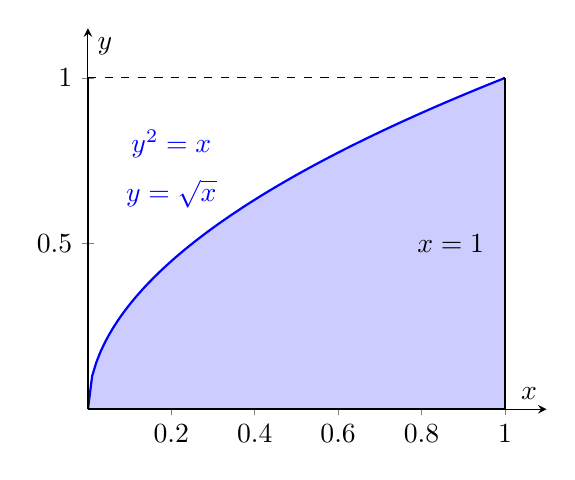
\begin{tikzpicture}
  \begin{axis}[
      axis lines = middle,
      xlabel = $x$, ylabel = $y$,
      domain=0:1,
      ymin=0, ymax=1.15,
      xmin=0, xmax=1.1,
      samples=100,
      clip=true,
      scale=0.85
    ]
    
    \addplot [
      name path=A,
      domain=0:1,
      draw=none,
    ] {sqrt(x)};

    \path[name path=B] (axis cs:0,1) -- (axis cs:1,1);
    \path[name path=C] (axis cs:0,0) -- (axis cs:0,1);
    \path[name path=D] (axis cs:0,0) -- (axis cs:1,0);

    \addplot [fill=blue!20, draw=none] fill between [of=D and A, soft clip={domain=0:1}];
    
    \addplot[blue, thick] {sqrt(x)};
    \addplot[thick] coordinates {(0,0) (0,1)};
    \addplot[thick] coordinates {(1,0) (1,1)};
    \addplot[thick] coordinates {(0,0) (1,0)};
    \draw[dashed] (axis cs: 0,1) -- (axis cs: 1,1);
    \node at (axis cs: 0.87, 0.5) {$x=1$};
    \node[blue] at (axis cs: 0.2, 0.8) {$y^2=x$};
    \node[blue] at (axis cs: 0.2, 0.65) {$y=\sqrt{x}$};

  \end{axis}
\end{tikzpicture}
\end{center}
\begin{align*}
\int_0^1\int_{y^2}^1y^3\cos\left(x^3\right)\,dx\,dy&=\int_0^1\int_0^{\sqrt x}y^3\cos\left(x^3\right)\,dy\,dx=\int_0^1\cos\left(x^3\right)\left[\frac{y^4}4\right]_{y=0}^{y=\sqrt x}\,dx\\\\&=\frac14\int_0^1x^2\cos\left(x^3\right)\,dx=\frac1{12}\bigg[\sin\left(x^3\right)\bigg]_0^1=\boxed{\frac1{12}\sin1}\end{align*}

\hfill

\noindent 4.


\hfill

\begin{minipage}{0.5\textwidth}

(i)

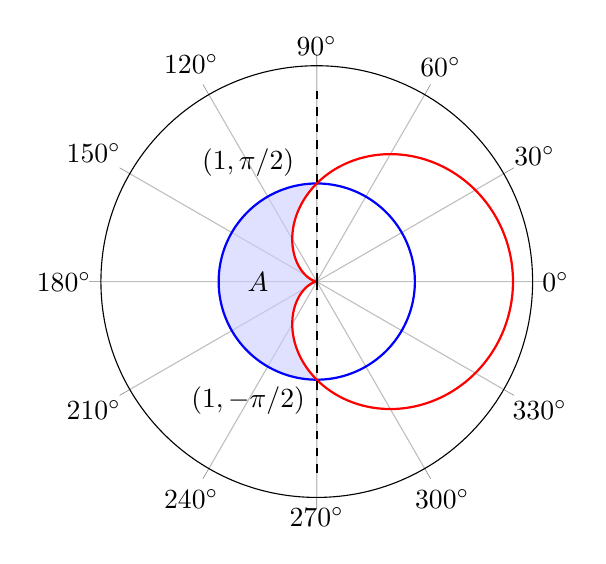
\begin{tikzpicture}
  \begin{polaraxis}[ytick=\empty, axis y line=none, scale=0.8, xticklabel=$\pgfmathprintnumber{\tick}^\circ$,]
    \addplot [
      domain=pi/2:3*pi/2,
      samples=300,
      draw=none,
      name path=A,
      data cs=polarrad,
    ] {1};

    \addplot [
      domain=pi/2:3*pi/2,
      samples=300,
      draw=none,
      name path=B,
      data cs=polarrad,
    ] {1+cos(deg(x))};

    \addplot [
      blue!20,
      fill opacity=0.6,
    ] fill between[of=A and B];

    \addplot [
      domain=0:2*pi,
      samples=300,
      thick,
      blue,
      data cs=polarrad,
    ] {1};

    \addplot [
      domain=0:2*pi,
      samples=300,
      thick,
      red,
      data cs=polarrad,
    ] {1+cos(deg(x))};

    \draw[black, thick, dashed] (axis cs: 90,0) -- (axis cs: 90,2);
    \draw[black, thick, dashed] (axis cs: -90,0) -- (axis cs: -90,2);

    \node at (axis cs:120,1.4) {$(1,\pi/2)$};
    \node at (axis cs:-120,1.4) {$(1,-\pi/2)$};
    \node at (0,-0.6) {$A$};

  \end{polaraxis}
\end{tikzpicture}
\end{minipage}
\begin{minipage}{0.4\textwidth}
\begin{equation*}
\text{(ii)}\quad\boxed{A=\int_{\pi/2}^{3\pi/2}\int_{1+\cos\theta}^1r\,dr\,d\theta}
\end{equation*}
\end{minipage}

\newpage

\noindent 5.

\hfill

\noindent (i)
\begin{center}
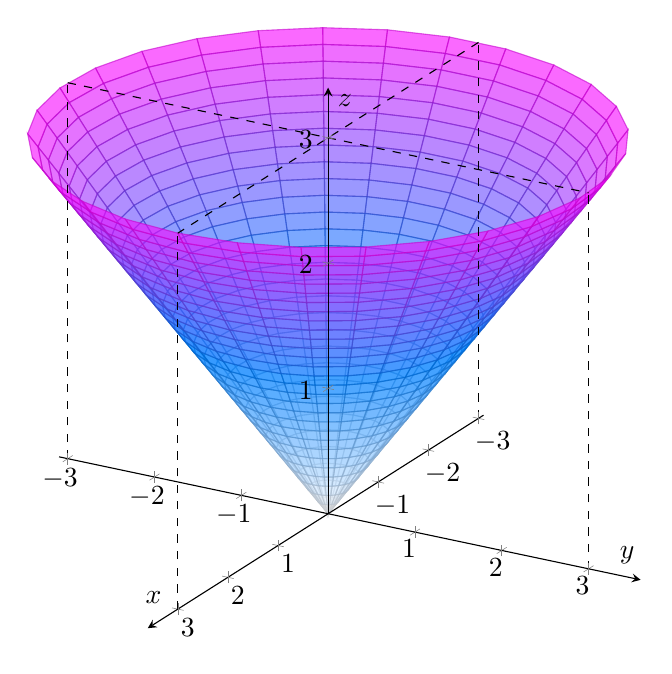
\begin{tikzpicture}
  \begin{axis}[
    view={120}{30},
    axis on top,
    axis lines=center,
    xlabel={$x$},
    ylabel={$y$},
    zlabel={$z$},
    xtick={-3,-2,-1,1,2,3},
    ytick={-3,-2,-1,1,2,3},
    xmin=-3.1, xmax=3.6,
    ymin=-3.1, ymax=3.6,
    zmin=0, zmax=3.4,
    samples=30,
    domain=0:360,
    y domain=0:3,
    scale=1.7,
  ]
  
\addplot3[surf, colormap/cool, z buffer=sort, opacity=0.6] ({y*cos(x)}, {y*sin(x)}, {y});

\draw[dashed] (axis cs:0,-3,3) -- (axis cs:0,3,3);
\draw[dashed] (axis cs:-3,0,3) -- (axis cs:3,0,3);

\draw[dashed] (axis cs:-3,0,0) -- (axis cs:-3,0,3);
\draw[dashed] (axis cs:0,3,0) -- (axis cs:0,3,3);
\draw[dashed] (axis cs:3,0,0) -- (axis cs:3,0,3);
\draw[dashed] (axis cs:0,-3,0) -- (axis cs:0,-3,3);

\end{axis}
\end{tikzpicture}
\end{center}
\begin{align*}
A&=\iint_D\sqrt{1+\left(\frac{\partial z}{\partial x}\right)^2 +\left(\frac{\partial z}{\partial y}\right)^2}\,dA= \iint_D\sqrt{1+\left(\frac{x}{\sqrt{x^2+y^2}}\right)^2 +\left(\frac{y}{\sqrt{x^2+y^2}}\right)^2}\,dA \\\\&=\iint_D\sqrt{1+\left(\frac{x^2+y^2}{x^2+y^2}\right)}\,dA=\iint_D\sqrt{1+1}\,dA=\sqrt{2}\iint_D\,dA
\end{align*}

\hfill

\noindent If we switch to polar coordinates, we can easily evaluate the integral.

\begin{equation*}A=\sqrt2\int_0^{2\pi}\int_0^3\,r\,dr\,d\theta=\sqrt2\int_0^{2\pi}\left[\frac{r^2}2\right]_{r=0}^{r=3}\,d\theta=\sqrt2\int_0^{2\pi}\frac92\,d\theta=\boxed{9\pi\sqrt2}\end{equation*}

\hfill

\noindent 6.

\hfill

\noindent (i) For spherical coordinates, we have

\[
\begin{array}{c}
z=\rho\cos\phi\\
r=\rho\sin\phi\\
x^2+y^2+z^2=\rho^2\\
dV=\rho^2\sin\phi\,d\rho\,d\phi\,d\theta
\end{array}\quad\rightarrow\quad
\begin{array}{lc}
z=8-x^2-y^2\implies\rho\cos\phi=8-\rho^2\sin^2\phi & (1)\\[0.2cm]
z=x^2+y^2\implies\rho\cos\phi=\rho^2\sin^2\phi & (2)\\
\end{array}
\]

\hfill

\noindent Now, notice that we have two distinct upper bounds for $\rho$. From $\phi=0$ to the angle of intersection, the integration is bounded above by $z=8-x^2-y^2$, where from the angle of intersection to $\phi=\pi/2$, the integration is bounded above by $z=x^2+y^2$.

\hfill

\noindent Solve $(1)$ for $\rho$ to find the upper bound.

\[\rho\cos\phi=8-\rho^2\sin^2\phi\implies\rho^2\sin^2\phi+\rho\cos\phi-8=0\]

\[\rho_{1,2}=\frac{-\cos\phi\pm\sqrt{\cos^2\phi-4\sin^2\phi\cdot(-8)}}{2\sin^2\phi}\quad\left[x_{1,2}=\frac{-b\pm\sqrt{b^2-4ac}}{2a}\right]\]

\[\rho>0\implies \rho_{\text{upper, 1}}=\frac{-\cos\phi+\sqrt{\cos^2\phi+32\sin^2\phi}}{2\sin^2\phi}\]

\hfill

\noindent Solve $(2)$ for $\rho$ to find the other upper bound.

\[\rho\cos\phi=\rho^2\sin^2\phi\implies\rho_{\text{upper, 2}}=\frac{\cos\phi}{\sin^2\phi}=\cot\phi\csc\phi\]

\hfill

\noindent Find where two surfaces intersect by equating $(1)$ and $(2)$.

\[8-\rho^2\sin^2\phi=\rho^2\sin^2\phi\implies \rho^2\sin^2\phi=4\implies \rho\sin\phi=2\implies r=2\]
\[z=x^2+y^2=r^2\implies z=4\implies \rho=\sqrt{x^2+y^2+z^2}=2\sqrt5\implies \sin\phi=\frac2\rho=\frac1{\sqrt{5}}\]
\[\phi=\arcsin\frac1{\sqrt5}\]

\hfill

\noindent We know $0\leq\theta\leq2\pi$. Therefore, the volume in spherical coordinates is as follows.

\begin{equation*}
\boxed{\begin{array}{ll}
V=&\displaystyle\int_0^{2\pi}\int_0^{\arcsin\textstyle\frac1{\sqrt5}}\int_0^{\textstyle\frac{-\cos\phi+\sqrt{\cos^2\phi+32\sin^2\phi}}{2\sin^2\phi}}\rho^2\sin\phi\,d\rho\,d\phi\,d\theta\\[1em]
&\displaystyle+\int_0^{2\pi}\int_{\arcsin\textstyle\frac1{\sqrt5}}^{\pi/2}\int_0^{\cot\phi\csc\phi}\rho^2\sin\phi\,d\rho\,d\phi\,d\theta
\end{array}}
\end{equation*}

\hfill

\noindent Since we choose the minimum of the bounds for $\rho$, we can write the equivalent expression.

\[\boxed{V=\displaystyle\int_0^{2\pi}\int_0^{\pi/2}\int_0^{\min\left(\cot\phi\csc\phi,\textstyle\frac{-\cos\phi+\sqrt{\cos^2\phi+32\sin^2\phi}}{2\sin^2\phi}\right)}\rho^2\sin\phi\,d\rho\,d\phi\,d\theta}\]

\hfill

\noindent (ii) For cylindrical coordinates, we have

\[
\begin{array}{c}
z=z\\
r^2=x^2+y^2\\
dV=r\,dz\,dr\,d\theta
\end{array}\quad\rightarrow\quad
\begin{array}{lc}
z=8-x^2-y^2\implies z=8-r^2 & (3)\\[1em]
z=x^2+y^2\implies z=r^2 & (4)\\
\end{array}
\]

\hfill

\noindent Equate $(3)$ and $(4)$ to find the upper bound for $r$.

\[8-r^2=r^2\implies r^2=4\implies r_{\text{upper}}=2\]

\hfill

\noindent The lower bound for $r$ is 0, and $0\leq\theta\leq2\pi$. The volume can be expressed as follows.

\[\boxed{V=\int_0^{2\pi}\int_0^2\int_{r^2}^{8-r^2}r\,dz\,dr\,d\theta}\]

\newpage


\begin{center}
2020-2021 Spring Final (09/06/2021) Solutions\\
(Last update: 05/08/2025 00:46)
\end{center}

\noindent 1.

\begin{minipage}{0.45\textwidth}
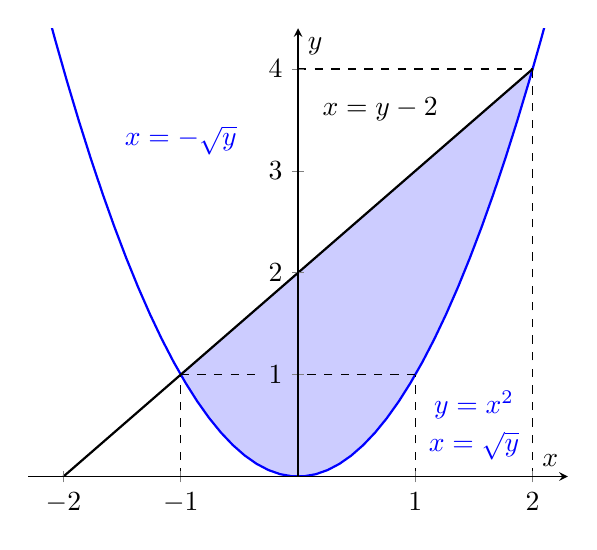
\begin{tikzpicture}
  \begin{axis}[
      axis lines = middle,
      xlabel = $x$, ylabel = $y$,
      ymin=0, ymax=4.4,
      xmin=-2.3, xmax=2.3,
      samples=100,
      clip=true,
      axis on top,
    ]
    
    \addplot [
      name path=A,
      domain=-2:2,
      draw=none,
    ] {x^2};

    \path[name path=B] (axis cs:-1,1) -- (axis cs:2,4);

    \addplot [
      fill=blue!20,
      draw=none,
    ] fill between [
      of=A and B,
      soft clip={domain=-1:2},
    ];
    
    \addplot[blue, thick] {x^2};
    \addplot[black, thick] coordinates {(-2,0) (2,4)};
    \draw[dashed] (axis cs:-1,1) -- (axis cs: -0.3,1);
    \draw[dashed] (axis cs:1,1) -- (axis cs: 0,1);
    \draw[dashed] (axis cs:2,0) -- (axis cs: 2,4);
    \draw[dashed] (axis cs:-1,0) -- (axis cs: -1,1);
    \draw[dashed] (axis cs:1,0) -- (axis cs: 1,1);
    \draw[dashed] (axis cs:0,4) -- (axis cs: 2,4);
    \node[blue] at (axis cs: 1.5, 0.7) {$y=x^2$};
    \node[blue] at (axis cs: 1.5, 0.3) {$x=\sqrt{y}$};
    \node[blue] at (axis cs: -1, 3.3) {$x=-\sqrt{y}$};
    \node at (axis cs: 0.7, 3.6) {$x=y-2$};

  \end{axis}
\end{tikzpicture}
\end{minipage}
\begin{minipage}{0.5\textwidth}
\begin{equation*}
\boxed{\int_0^1\int_{-\sqrt y}^{\sqrt y}\,dx\,dy+\int_1^4\int_{y-2}^{\sqrt y}\,dx\,dy}\end{equation*}
\end{minipage}

\hfill

\noindent 2. Using polar coordinates, we can find the volume with a double integral.

\[
\begin{array}{c}
r^2=x^2+y^2\\
dA=r\,dr\,d\theta
\end{array}\quad\rightarrow\quad
\begin{array}{c}z=\sqrt{x^2+y^2}\implies z=\sqrt{r^2}\implies z=r\\[0.3cm]
x^2+y^2\leq4\,\rightarrow\,r^2\leq4\implies 0\leq r\leq 2\\[0.3cm]
0\leq\theta\leq2\pi
\end{array}
\]

\begin{align*}\text{Volume}&=\int_0^{2\pi}\int_{0}^{2}\left[r-0\right]\cdot r\,dr\,d\theta=\int_0^{2\pi}\int_{0}^{2}r^2\,dr\,d\theta=\int_0^{2\pi}\left[\frac{r^3}3\right]_{r=0}^{r=2}d\theta\\\\&=\frac83\int_0^{2\pi}\,d\theta=\boxed{\frac{16\pi}3}\end{align*}

\hfill

\noindent 3.

\hfill

\begin{minipage}{0.5\textwidth}

(i)

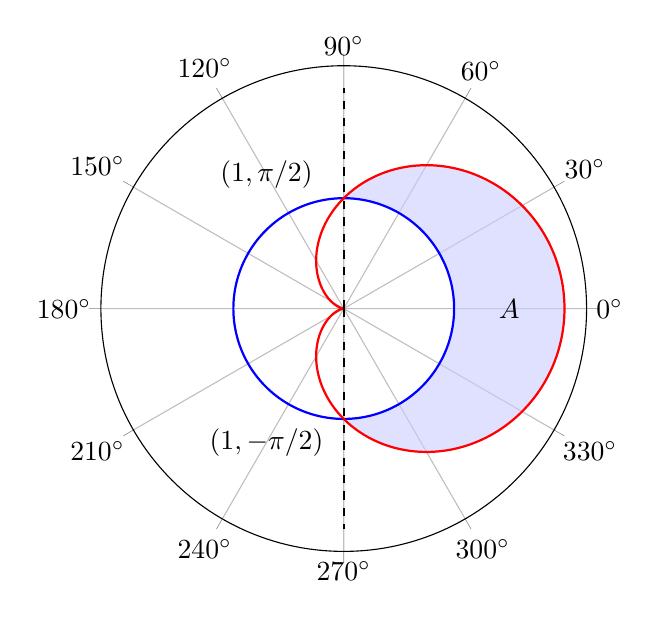
\begin{tikzpicture}
  \begin{polaraxis}[ytick=\empty, axis y line=none, scale=0.9, xticklabel=$\pgfmathprintnumber{\tick}^\circ$,]
    \addplot [
      domain=-pi/2:pi/2,
      samples=300,
      draw=none,
      name path=A,
      data cs=polarrad,
    ] {1};

    \addplot [
      domain=-pi/2:pi/2,
      samples=300,
      draw=none,
      name path=B,
      data cs=polarrad,
    ] {1+cos(deg(x))};

    \addplot [
      blue!20,
      fill opacity=0.6,
    ] fill between[of=A and B];

    \addplot [
      domain=0:2*pi,
      samples=300,
      thick,
      blue,
      data cs=polarrad,
    ] {1};

    \addplot [
      domain=0:2*pi,
      samples=300,
      thick,
      red,
      data cs=polarrad,
    ] {1+cos(deg(x))};

    \draw[black, thick, dashed] (axis cs: 90,0) -- (axis cs: 90,2);
    \draw[black, thick, dashed] (axis cs: -90,0) -- (axis cs: -90,2);

    \node at (axis cs:120,1.4) {$(1,\pi/2)$};
    \node at (axis cs:-120,1.4) {$(1,-\pi/2)$};
    \node at (0,1.5) {$A$};

  \end{polaraxis}
\end{tikzpicture}
\end{minipage}
\begin{minipage}{0.4\textwidth}
\begin{equation*}
\text{(ii)}\quad\boxed{A=\int_{-\pi/2}^{\pi/2}\int_1^{1+\cos\theta}r\,dr\,d\theta}
\end{equation*}
\end{minipage}

\newpage

\noindent 4.

\hfill

\noindent (i)

\begin{center}
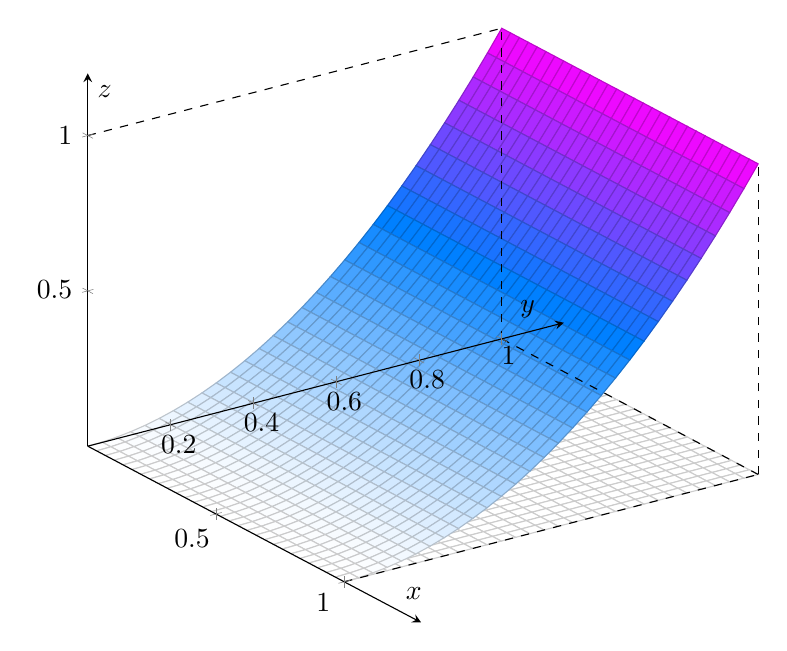
\begin{tikzpicture}
  \begin{axis}[
      view={55}{30},
      axis lines=center,
      xlabel=$x$, ylabel=$y$, zlabel=$z$,
      xmin=0, xmax=1.3,
      ymin=0, ymax=1.15,
      zmin=0, zmax=1.2,
      samples=30,
      domain=0:1,
      y domain=0:1,
      colormap/cool,
      mesh/ordering=y varies,
      scale=1.5,
      axis on top,
    ]
    
    \addplot3[surf]{0};
    \addplot3[surf]{y^2};

    \draw[dashed] (axis cs:0,1,0)--(axis cs:0,1,1);
    \draw[dashed] (axis cs:1,0,0)--(axis cs:1,1,0);
    \draw[dashed] (axis cs:0,1,0)--(axis cs:1,1,0);
    \draw[dashed] (axis cs:1,1,0)--(axis cs:1,1,1);
    \draw[dashed] (axis cs:0,0,1)--(axis cs:0,1,1);

   \end{axis}
\end{tikzpicture}
\end{center}

\hfill

\noindent (ii) Calculate the partial derivatives to find the surface area.

\begin{equation*}
z=y^2\implies\quad\frac{\partial z}{\partial x}=0,\quad \frac{\partial z}{\partial y}=2y
\end{equation*}

\hfill

\begin{align*}\text{Surface area}&=\iint_D\sqrt{1+\left(\frac{\partial z}{\partial x}\right)^2+\left(\frac{\partial z}{\partial y}\right)^2}\,dA=\int_0^1\int_0^1\sqrt{1+\left(0\right)^2+\left(2y\right)^2}\,dx\,dy\\\\&=\int_0^1\int_0^1\sqrt{4y^2+1}\,dx\,dy=\int_0^1\left[x\sqrt{4y^2+1}\right]_{x=0}^{x=1}\,dy\\\\&=\int_0^1\sqrt{4y^2+1}\,dy\:\left[y=\frac12\tan u \implies dy=\frac12\sec^2u\,du,\:\begin{array}{l}u_{\text{upper}}=\arctan2\\u_{\text{lower}}=0\end{array}\right]\\\\&=\frac12\int_0^{\arctan2}\sqrt{\tan^2u+1}\cdot\sec^2u\,du=\frac12\int_0^{\arctan2}\sec^3u\,du\end{align*}

\hfill

\noindent To evaluate the last integral, we will use integration by parts.

\begin{align*}
    w=\sec u\,&\rightarrow\, dw = \sec u\tan u \,du\\
    dz=\sec^2u\,du\,&\rightarrow\, z = \tan u
\end{align*}
\begin{align*}
\int_0^{\arctan2}\sec^3u\,du&=\tan u \cdot \sec u\,\bigg|_0^{\arctan2} -\int_0^{\arctan2} \tan^2 u\sec u\, du\\\\&= \tan u \cdot \sec u\,\bigg|_0^{\arctan2} -\int_0^{\arctan2} \frac{1-\cos^2u}{\cos^3 u}\, du\\\\&= \tan u \cdot \sec u\,\bigg|_0^{\arctan2} - \int_0^{\arctan2} \sec^3u \, du + \int_0^{\arctan2} \sec u \, du 
\end{align*}

\hfill

\noindent Notice that the integral we want to evaluate appears on the right side. After a little algebra, we can evaluate the integral.

\begin{equation*}
\int_0^{\arctan2}\sec^3u\,du=\frac12\cdot\tan u\cdot\sec u\,\bigg|_0^{\arctan2}+\frac12\cdot\int_0^{\arctan2}\sec u\,du
\end{equation*}

\hfill

\noindent The integral of $\sec u$ with respect to $u$ is as follows. One can derive it with particular methods.

\begin{equation*}\int_0^{\arctan2}\sec u \, du = \ln\left|\tan u + \sec u\right|\bigg|_0^{\arctan2}
\end{equation*}

\hfill

\noindent So, the surface area becomes as follows.

\begin{align*}\text{Surface area}&=\frac12\int_0^{\arctan2}\sec^3u\,du=\frac14\left(\tan u\cdot\sec u+\ln\left|\tan u+\sec u\right|\right)\bigg|_0^{\arctan2}\\\\&=\frac14\left[2\sec(\arctan2)+ \ln(2+\sec(\arctan2))-0\right]=\boxed{\frac14\left[2\sqrt5+\ln\left(2+\sqrt5\right)\right]}\end{align*}

\hfill

\noindent 5. By means of spherical coordinates, we can easily evaluate the integral. For spherical coordinates, we have

\[
\begin{array}{c}
z=\rho\cos\theta\\
r=\rho\sin\theta\\
x^2+y^2+z^2=\rho^2\\
dV=\rho^2\sin\phi\,d\rho\,d\phi\,d\theta
\end{array}\quad\rightarrow\quad
\begin{array}{c}
x^2+y^2+z^2=4\,\rightarrow\,\rho^2 = 4\implies \rho_{\text{min}}=2\\
x^2+y^2+z^2=9\,\rightarrow\,\rho^2 = 9\implies \rho_{\text{max}}=3\\
z\equiv\rho\cos\phi\\
0\leq\theta\leq2\pi,\quad0\leq\phi\leq\pi
\end{array}
\]

\begin{align*}
\iiint_Ez\,dV&=\int_0^{2\pi}\int_0^\pi\int_2^3\rho\cos\phi\cdot\rho^2\sin\phi\,d\rho\,d\phi\,d\theta=\frac12\int_0^{2\pi}\int_0^\pi\int_2^3\rho^3\sin(2\phi)\,d\rho\,d\phi\,d\theta\\\\&=\frac12\int_0^{2\pi}\int_0^\pi\left[\frac{\rho^4}{4}\right]_{\rho=2}^{\rho=3}\sin(2\phi)\,d\phi\,d\theta=\frac{65}{8}\int_0^{2\pi}\int_0^\pi\sin(2\phi)\,d\phi\,d\theta\\\\&=\frac{65}{8}\int_0^{2\pi}\left[-\frac12\cos(2\phi)\right]_{\phi=0}^{\phi=\pi}\,d\theta=\frac{65}{8}\int_0^{2\pi}0\,d\theta =\boxed0
\end{align*}

\newpage

\noindent 6.

\hfill

\noindent (i) For spherical coordinates, we have

\[
\begin{array}{c}
z=\rho\cos\phi\\
r=\rho\sin\phi\\
x^2+y^2+z^2=\rho^2\\
dV=\rho^2\sin\phi\,d\rho\,d\phi\,d\theta
\end{array}\quad\rightarrow\quad
\begin{array}{cc}
z=1-x^2-y^2\implies\rho\cos\phi=1-\rho^2\sin^2\phi&(1)\\[0.3cm]
\displaystyle0\leq\phi\leq\frac\pi2,\quad0\leq\theta\leq2\pi,\quad0\leq\rho\leq\rho_{\text{upper}}
\end{array}
\]

\hfill

\noindent Find $\rho_{\text{upper}}$ with equation $(1)$.

\[
\begin{array}{c}
\rho\cos\phi=1-\rho^2\sin^2\phi\implies \rho^2\sin^2\phi+\rho\cos\phi-1=0\\\\
\displaystyle \rho_{1,2} = \frac{-\cos\phi \pm\sqrt{\cos^2\phi-4\cdot\sin^2\phi\cdot(-1)}}{2\sin^2\phi}\quad\left[x_{1,2}=\frac{-b\pm\sqrt{b^2-4ac}}{2a}\right]\\\\
\displaystyle \rho>0\implies\rho_{\text{upper}}=\frac{-\cos\phi +\sqrt{\cos^2\phi+4\sin^2\phi}}{2\sin^2\phi}
\end{array}
\]

\hfill

\[\boxed{\text{Volume}=\int_0^{2\pi}\int_0^{\pi/2}\int_0^{\textstyle\frac{-\cos\phi +\sqrt{\cos^2\phi+4\sin^2\phi}}{2\sin^2\phi}}\rho^2\sin\phi\,d\rho\,d\phi\,d\theta}\]

\hfill

\noindent (ii) For cylindrical coordinates, we have

\[
\begin{array}{c}
z=z\\
r^2=x^2+y^2\\
dV=r\,dz\,dr\,d\theta
\end{array}\quad\rightarrow\quad
\begin{array}{c}
z=1-x^2-y^2\implies z=1-r^2\\
0\leq\theta\leq2\pi,\quad 0\leq r \leq1
\end{array}
\]

\[\boxed{\text{Volume}=\int_0^{2\pi}\int_0^1\int_0^{1-r^2}r\,dz\,dr\,d\theta}\]

\newpage


\begin{center}
2021-2022 Spring Final (23/05/2022) Solutions\\
(Last update: 05/08/2025 01:58)
\end{center}

\noindent 1) Let $g(x,y)=x+y-1$ and then, solve the system of equations below using the method of Lagrange multipliers.

\[
\left.
\begin{array}{ll}
\displaystyle\nabla f =\lambda \nabla g \\
\displaystyle g(x,y) = 0
\end{array}
\right\}\quad
\begin{array}{ll}
\nabla f = \left\langle 2x, 2y\right\rangle = \lambda\left\langle1,1\right\rangle = \lambda\nabla g\\\therefore\displaystyle \lambda = 2x\quad \text{and}\quad \lambda = 2y\quad \text{and}\quad x+y-1=0
\end{array}
\]

\[\lambda=2x=2y\implies x=y\]
\[x+y-1=0 \,\rightarrow\, 2x-1 = 0\,\rightarrow\,x=\frac12=y\]

\hfill

\noindent Evaluate $\displaystyle f\left(\frac12,\frac12\right)$ to find the minimum value.

\[f\left(\frac12,\frac12\right)=\left(\frac12\right)^2+\left(\frac12\right)^2=\frac12\]

\hfill

\noindent $f(x,y)$ is defined for $x\geq0$ and $y\geq0$. This implies that $0\leq y \leq1$ and $0\leq x\leq1$ by the constraint. The domain of $f$ is closed and bounded, and $f$ is continuous. By the extreme value theorem, the absolute minima and maxima must exist. Using the method of Lagrange multipliers, we could find only one point. This means that the other value exists on the boundary of $f$.

\[x=0\,\rightarrow\,0+y-1=0\,\rightarrow\,y=1,\quad y=0\,\rightarrow\, x+0-1=0\,\rightarrow\, x=1\]
\[f(0,1) = 0^2 +1^2 = 1,\quad f(1,0) = 1^2+0^2 = 1\]

\hfill

\noindent Eventually, compare the values we obtain.

\[\boxed{\frac12\,\text{is the absolute minimum}, 1\,\text{is the absolute maximum}.}\]

\hfill

\noindent 2)

\begin{center}
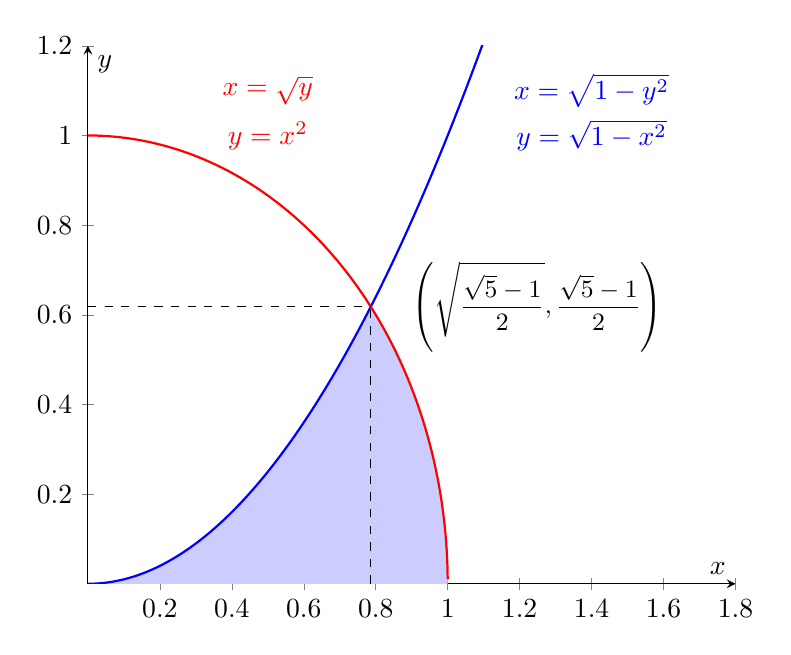
\begin{tikzpicture}
  \begin{axis}[
      axis lines=center,
      xlabel={$x$},
      ylabel={$y$},
      xmin=0, xmax=1.8,
      ymin=0, ymax=1.2,
      samples=200,
      clip=true,
      scale=1.2,
    ]
    
    \addplot [
        fill=blue!20,
        domain=0:0.786,
        draw=none,
    ] {x^2} \closedcycle;
    
    \addplot [
        fill=blue!20,
        domain=0.784:1,
        draw=none,
    ] {sqrt(1-x^2)} \closedcycle;

    \addplot [
        thick,
        blue,
        domain=0:1.1,
        samples=200,
    ] {x^2};

    \addplot [
        thick,
        red,
        domain=0:1.1,
        samples=3200,
    ] {sqrt(1-x^2)};

    \node[blue] at (axis cs:1.4,1.1) {$x = \sqrt{1 - y^2}$};
    \node[red] at (axis cs:0.5,1.1) {$x = \sqrt{y}$};
    \node[blue] at (axis cs:1.4,1) {$y = \sqrt{1 - x^2}$};
    \node[red] at (axis cs:0.5,1) {$y=x^2$};
    \node at (axis cs:1.25,0.618) {\small$\displaystyle\left(\sqrt{\frac{\sqrt5-1}{2}},\frac{\sqrt5-1}2\right)$};

    % Label y-max
    \draw[dashed] (axis cs:0,0.618) -- (axis cs:{sqrt(0.618)},0.618);
    \draw[dashed] (axis cs:0.786,0) -- (axis cs:0.786,0.618);

    \node[left] at (axis cs:0,0.618) {\footnotesize $\frac{-1+\sqrt{5}}{2}$};

  \end{axis}
\end{tikzpicture}
\end{center}

\hfill

\noindent The integral with reverse order is as follows.

\begin{equation*}
\boxed{\int_0^{\sqrt{\frac{\sqrt5 - 1}2}}\int_0^{x^2}\,dy\,dx + \int_{\sqrt{\frac{\sqrt5 - 1}2}}^{1}\int_0^{\sqrt{1-x^2}}\,dy\,dx}
\end{equation*}

\hfill

\noindent 3) Find where these two curves intersect and then find the area.

\[1=1+\sin\theta\implies\sin\theta=0\implies\theta=k\pi,\quad k\in\mathbb{Z}\]


\begin{center}
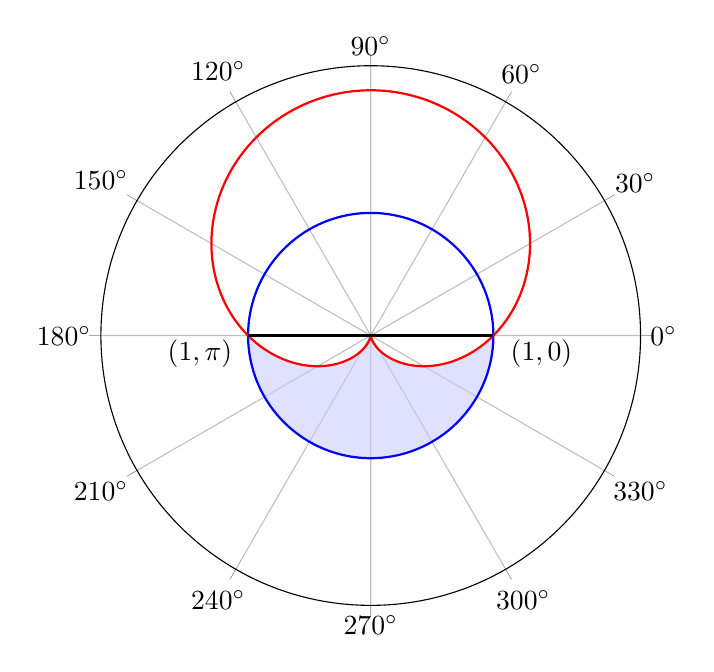
\begin{tikzpicture}
  \begin{polaraxis}[ytick=\empty, axis y line=none, xticklabel=$\pgfmathprintnumber{\tick}^\circ$,]
    \addplot [
      domain=pi:2*pi,
      samples=300,
      draw=none,
      name path=A,
      data cs=polarrad,
    ] {1};

    \addplot [
      domain=pi:2*pi,
      samples=300,
      draw=none,
      name path=B,
      data cs=polarrad,
    ] {1+sin(deg(x))};

    \addplot [
      blue!20,
      fill opacity=0.6,
    ] fill between[of=A and B];

    \addplot [
      domain=0:2*pi,
      samples=300,
      thick,
      blue,
      data cs=polarrad,
    ] {1};

    \addplot [
      domain=0:2*pi,
      samples=300,
      thick,
      red,
      data cs=polarrad,
    ] {1+sin(deg(x))};

    \draw[black, thick] (axis cs: 0,-1) -- (axis cs: 0,1);
    \node at (axis cs: 6,-1.4) {$(1,\pi)$};
    \node at (axis cs: -6,1.4) {$(1,0)$};

  \end{polaraxis}
\end{tikzpicture}
\end{center}
\begin{align*}
\text{Area}&=\int_{\pi}^{2\pi}\int_{1+\sin\theta}^1\,r\,dr\,d\theta=\frac12\int_\pi^{2\pi}\left[1^2-(1+\sin\theta)^2\right]\,d\theta\\\\&=\frac12\int_\pi^{2\pi}\left[-2\sin\theta-\sin^2\theta\right]\,d\theta\quad\left[\sin^2\theta+\cos^2\theta=1\right]\\\\&=-\int_\pi^{2\pi}\sin\theta\,d\theta-\frac12\int_\pi^{2\pi}(1-\cos^2\theta)\,d\theta\quad[2\cos^2\theta-1=\cos(2\theta)] \\\\&=-\int_\pi^{2\pi}\sin\theta\,d\theta+\int_\pi^{2\pi}\frac{\cos(2\theta)-1}{4}\,d\theta=\int_\pi^{2\pi}\left[-\frac14+\frac14\cos(2\theta)-\sin\theta\right]\,d\theta\\\\&=\left[-\frac\theta4+\frac18\sin(2\theta)+\cos\theta\right]_{\pi}^{2\pi}=\left[\left(-\frac{\pi}2+0+1\right)-\left(-\frac{\pi}4+0-1\right)\right]={\boxed{2-\frac{\pi}4}}
\end{align*}

\hfill

\noindent 4) We have the sphere $x^2+y^2+z^2=16$. So, the upper bound is $z=\sqrt{16-x^2-y^2}$, while the lower bound is $z=0$. If we project the domain onto the $xy$-plane, we see that the upper and lower bounds for $y$ are $\sqrt{2-x^2}$ and $-\sqrt{2-x^2}$, respectively. For $x$, the integration starts from $-\sqrt2$ and ends at $\sqrt2$. The volume of the object can be evaluated using the following integral.

\newpage

\begin{equation*}\mathrm{I}=\int_{-\sqrt2}^{\sqrt2}\int_{-\sqrt{2-x^2}}^{\sqrt{2-x^2}}\left[\sqrt{16-x^2-y^2}-0 \right]\,dy\,dx\end{equation*}

\hfill

\noindent This integral seems a little bit hard. We can switch to polar coordinates for ease. Use the transformation below.

\[
\begin{array}{c}
x^2+y^2=r^2\\
dA=dy\,dx =r\,dr\,d\theta
\end{array}\quad\rightarrow\quad
\begin{array}{c}
0\leq z\leq\sqrt{16-r^2}\\
0\leq r\leq \sqrt2\\
0\leq\theta\leq 2\pi\\
\end{array} 
\]
\begin{align*}\mathrm{I}&=\int_{0}^{2\pi}\int_{0}^{\sqrt{2}}\sqrt{16-r^2}\,r\,dr\,d\theta=\int_{0}^{2\pi}\left[-\frac13\left(16-r^2\right)^{3/2}\right]_{r=0}^{r=\sqrt2}\,d\theta\\\\&=\frac13\int_0^{2\pi}\left[-14^{3/2}-\left(-16^{3/2}\right)\right]\,d\theta=\boxed{\frac{2\pi}{3}\left(16^{3/2}-14^{3/2}\right)}
\end{align*}

\hfill

\noindent 5)

\hfill

\noindent (i)
\begin{center}
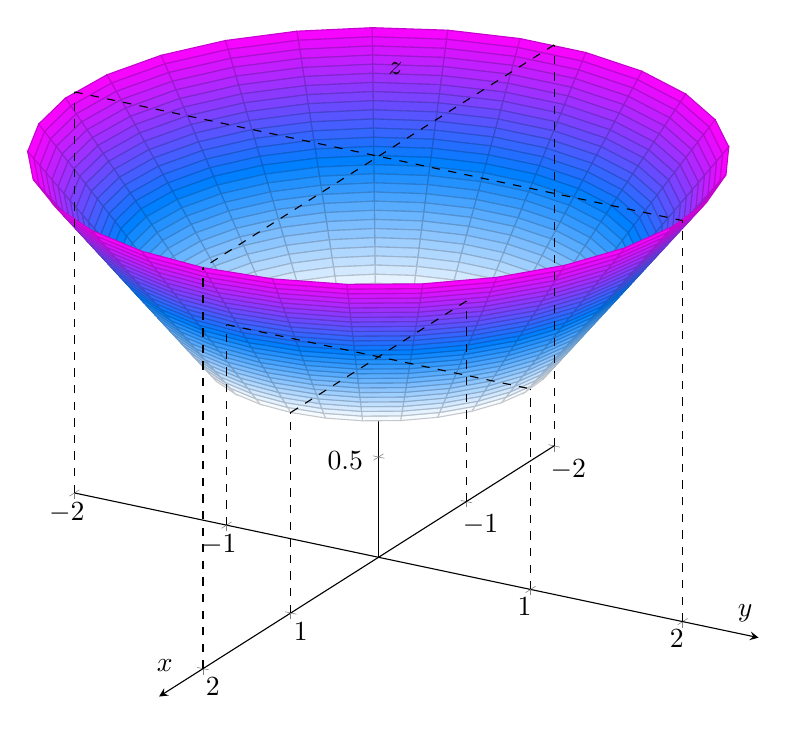
\begin{tikzpicture}
  \begin{axis}[
    view={120}{30},
    axis lines=center,
    xlabel={$x$},
    ylabel={$y$},
    zlabel={$z$},
    xtick={-2,-1,1,2},
    ytick={-2,-1,1,2},
    xmin=-2, xmax=2.5,
    ymin=-2, ymax=2.5,
    zmin=0, zmax=2.5,
    samples=30,
    domain=0:360,
    colormap/cool,
    scale=2,
  ]
    \addplot3[
      surf,
      z buffer=sort,
      y domain=1:2,
    ]
    ({y*cos(x)}, {y*sin(x)}, {y});
%\addplot3[y domain=0:1, dashed, samples = 10]({y*cos(x)}, {y*sin(x)}, {y});
    
\draw[dashed] (axis cs:0,-2,2) -- (axis cs: 0, 2, 2);
\draw[dashed] (axis cs:-2,0,2) -- (axis cs: 2, 0,2);
\draw[dashed] (axis cs:-1,0,1) -- (axis cs: 1, 0, 1);
\draw[dashed] (axis cs:0,-1,1) -- (axis cs: 0, 1,1);

\draw[dashed] (axis cs:-2,0,0) -- (axis cs: -2, 0, 2);
\draw[dashed] (axis cs:0,2,0) -- (axis cs: 0,2,2);
\draw[dashed] (axis cs:2,0,0) -- (axis cs: 2, 0, 2);
\draw[dashed] (axis cs:0,-2,0) -- (axis cs: 0, -2,2);

\draw[dashed] (axis cs:-1,0,0) -- (axis cs: -1, 0, 1);
\draw[dashed] (axis cs:0,1,0) -- (axis cs: 0,1,1);
\draw[dashed] (axis cs:1,0,0) -- (axis cs: 1, 0, 1);
\draw[dashed] (axis cs:0,-1,0) -- (axis cs: 0, -1,1);

\end{axis}
\end{tikzpicture}
\end{center}

\hfill

\noindent (ii) Using the double integral below, we find the lateral surface area.

\begin{align*}
A&=\iint_D\sqrt{1+\left(\frac{\partial z}{\partial x}\right)^2 +\left(\frac{\partial z}{\partial y}\right)^2}\,dA= \iint_D\sqrt{1+\left(\frac{x}{\sqrt{x^2+y^2}}\right)^2 +\left(\frac{y}{\sqrt{x^2+y^2}}\right)^2}\,dA \\\\&=\iint_D\sqrt{1+\left(\frac{x^2+y^2}{x^2+y^2}\right)}\,dA=\iint_D\sqrt{1+1}\,dA=\sqrt{2}\iint_D\,dA
\end{align*}

\newpage

\noindent If we switch to polar coordinates, we can easily evaluate the integral.

\begin{equation*}A=\sqrt2\int_0^{2\pi}\int_1^2\,r\,dr\,d\theta=\sqrt2\int_0^{2\pi}\left[\frac{r^2}2\right]_{r=1}^{r=2}\,d\theta=\sqrt2\int_0^{2\pi}\frac32\,d\theta=\boxed{3\pi\sqrt2}\end{equation*}

\hfill

\noindent 6)

\hfill

\noindent (i) For spherical coordinates, we have

\[
\begin{array}{c}
z=\rho\cos\phi\\
r=\rho\sin\phi\\
x^2+y^2+z^2=\rho^2\\
dV=\rho^2\sin\phi\,d\rho\,d\phi\,d\theta
\end{array}\quad\rightarrow\quad
\begin{array}{c}
x^2+y^2=1\,\rightarrow\,\rho^2\sin^2\phi = 1\\
z=6\,\rightarrow\,\rho\cos\phi=6\\
z=1-x^2-y^2\,\rightarrow\,\rho\cos\phi=1-\rho^2\sin^2\phi
\end{array}
\]

\hfill

\noindent We have the lower bound for $\rho$, which is the solution of $\rho\cos\phi=1-\rho^2\sin^2\phi$

\[
\begin{array}{c}
\rho\cos\phi=1-\rho^2\sin^2\phi\\\\
\rho^2\sin^2\phi+\rho\cos\phi-1=0\\\\
\displaystyle \rho_{1,2} = \frac{-\cos\phi \pm\sqrt{\cos^2\phi-4\cdot\sin^2\phi\cdot(-1)}}{2\sin^2\phi}\quad\left[x_{1,2}=\frac{-b\pm\sqrt{b^2-4ac}}{2a}\right]\\\\
\displaystyle \rho>0\implies\rho_{\text{lower}}=\frac{-\cos\phi +\sqrt{\cos^2\phi+4\sin^2\phi}}{2\sin^2\phi}
\end{array}
\]

\hfill

\noindent However, we have two distinct upper bounds for $\rho$. We need to find the value of $\phi$ where the surfaces $\rho\cos\phi = 6$ and $\rho^2\sin^2\phi=1$ intersect.

\begin{equation*}
\rho^2\sin^2\phi=1 \,\rightarrow\,\rho\sin\phi = 1
\end{equation*}

\[
\left.
\begin{array}{c}
\rho\sin\phi=1\\
\rho\cos\phi=6
\end{array}
\right\}\quad\tan\phi=\frac16\implies\phi=\arctan{\frac16}
\]

\hfill

\noindent For $\displaystyle\phi<\arctan\frac16$, the upper bound is $\displaystyle \frac6{\cos\phi}$. Meanwhile, for $\displaystyle\phi>\arctan\frac16$, it is $\displaystyle \frac1{\sin\phi}$.

\hfill

\noindent The region in the $xy-$plane is circular, therefore $0\leq\theta\leq2\pi$. As for $\phi$, we have $\displaystyle0\leq\phi\leq\frac{\pi}2$. The volume of the object in spherical coordinates can be expressed as follows.

\begin{equation*}
\boxed{\begin{array}{cc}
V=&\displaystyle\int_0^{2\pi}\int_0^{\arctan{\textstyle\frac16}}\int_{\textstyle\frac{-\cos\phi +\sqrt{\cos^2\phi+4\sin^2\phi}}{2\sin^2\phi}}^{\textstyle\frac6{\cos\phi}}\,\rho^2\sin\phi\,d\rho\,d\phi\,d\theta\\
&\displaystyle+\int_0^{2\pi}\int_{\arctan{\textstyle\frac16}}^{\pi/2}\int_{\textstyle\frac{-\cos\phi +\sqrt{\cos^2\phi+4\sin^2\phi}}{2\sin^2\phi}}^{\textstyle\frac1{\sin\phi}}\,\rho^2\sin\phi\,d\rho\,d\phi\,d\theta 
\end{array}}
\end{equation*}

\hfill

\noindent In fact, we are looking for the minimum value of the upper bound for $\rho$ between $\displaystyle\frac1{\sin\phi}$ and $\displaystyle\frac6{\cos\phi}$. Hence, we can write the equivalent expression as follows.

\begin{equation*}
\boxed{V=\displaystyle\int_0^{2\pi}\int_0^{\pi/2}\int_{\textstyle\frac{-\cos\phi +\sqrt{\cos^2\phi+4\sin^2\phi}}{2\sin^2\phi}}^{\min\left(\textstyle\frac6{\cos\phi},\frac1{\sin\phi}\right)}\,\rho^2\sin\phi\,d\rho\,d\phi\,d\theta}
\end{equation*}

\hfill

\noindent (ii) For cylindrical coordinates, we have

\[
\begin{array}{c}
z=z\\
r^2=x^2+y^2\\
dV=r\,dz\,dr\,d\theta
\end{array}\quad\rightarrow\quad
\begin{array}{c}
x^2+y^2=1\,\rightarrow\,r^2 = 1\,\rightarrow\,r=1\\
z=6\\
z=1-x^2-y^2\,\rightarrow\,z=1-r^2
\end{array}
\]

\hfill

\noindent The volume can be expressed as follows.

\begin{align*}
    V&=\int_0^{2\pi}\int_0^1\int_{1-r^2}^{6}\,r\,dz\,dr\,d\theta=\int_0^{2\pi}\int_0^1\big[z\big]_{z=1-r^2}^{z=6}\,r\,dr\,d\theta\\\\&=\int_0^{2\pi}\int_0^1\left(r^3+5r\right)\,dr\,d\theta=\int_0^{2\pi}\left[\frac{r^4}{4} + \frac{5r^2}{2}\right]_{r=0}^{r=1}\,d\theta\\\\&=\big[\theta\big]_0^{2\pi}\cdot\left[ \left(\frac{1^4}4 + \frac{5\cdot1^2}2\right)-\left(0\right)\right]=\boxed{\frac{11\pi}2}
\end{align*}

\newpage


\begin{center}
2022-2023 Spring Final (12/06/2023) Solutions\\
(Last update: 05/08/2025 00:53)
\end{center}

\noindent 1. Let $g(x,y,z)=x^2+y^2+z^2-4$ and then solve the system of equations below using the method of Lagrange multipliers.

\[
\left.
\begin{array}{ll}
\displaystyle\nabla f =\lambda \nabla g \\
\displaystyle g(x,y,z) = 0
\end{array}
\right\}\quad
\begin{array}{ll}
\nabla f = \left\langle y^2z,2xyz,xy^2\right\rangle = \lambda\left\langle2x,2y,2z\right\rangle = \lambda\nabla g \\[0.2cm] x^2+y^2+z^2-4=0
\end{array}
\]

\[
\left.
\begin{array}{ll}
\displaystyle y^2z =\lambda \cdot2x & (1)\\[0.2cm]
\displaystyle 2xyz =\lambda \cdot2y & (2)\\[0.2cm]
\displaystyle xy^2 =\lambda \cdot2z & (3)\\[0.2cm]
\end{array}
\right\}\quad
\begin{array}{ll}
\displaystyle(1)\,\&\,(3)\rightarrow\frac{z}{x}=\frac{x}{z}\rightarrow x^2=z^2\rightarrow x=\pm z&(4)\\[0.4cm]
\displaystyle(1)\,\&\,(2)\rightarrow\frac{y}{2x}=\frac{x}{y}\rightarrow y^2=2x^2\rightarrow y=\pm\sqrt{2}x&(5)\\[0.4cm]\displaystyle(4)\,\&\,(5)\rightarrow y=\pm \sqrt 2z
\end{array}
\]

\hfill

\noindent Now, use the constraint to find the coordinates. Write $y$ and $z$ in terms of $x$.

\[x^2+y^2+z^2-4=0\implies x^2+\left(\sqrt2x\right)^2+x^2-4=0\implies4x^2=4\implies x=\pm1\]
\[\therefore y=\pm\sqrt2,\quad z=\pm1\]

\hfill

\noindent Evaluate $f$ at either of these points: $(1,\sqrt2,1)$, $(-1,\sqrt2,-1)$, $(-1,-\sqrt2,-1)$.

\[f_{\text{max}}=f(1,\sqrt2,1)=1\cdot\left(\sqrt2\right)^2\cdot1=\boxed{2}\]

\hfill

\noindent 2.

\begin{center}
\begin{tikzpicture}
  \begin{axis}[
      axis lines=center,
      xlabel={$x$},
      ylabel={$y$},
      xmin=0, xmax=1.2,
      ymin=0, ymax=1.2,
      samples=200,
      clip=true,
      scale=1.2,
    ]
    
    \addplot [
        fill=blue!20,
        domain=0:1,
        draw=none,
    ] {1} \closedcycle;
    
    \addplot [
        fill=white,
        domain=0:1,
        draw=none,
    ] {x^(1/4)} \closedcycle;

    \addplot [
        thick,
        blue,
        domain=0:1.1,
    ] {1};

    \addplot [
        thick,
        red,
        domain=0:1.1,
        samples=200,
    ] {x^(1/4)};

    \node[blue] at (axis cs: 0.2, 1.1) {\large $y=1$};
    \node[red] at (axis cs: 0.4, 0.6) {\large $y=x^{1/4}$};
    \node[red] at (axis cs: 0.4, 0.5) {\large $x=y^4$};

  \end{axis}
\end{tikzpicture}
\end{center}

\hfill

\noindent The integral given with this order is difficult to evaluate. Change the order of integration.

\begin{align*}\int_0^1\int_{x^{1/4}}^1\,\mathrm{e}^{y^5}dy\,dx=\int_0^1\int_0^{y^4}\mathrm{e}^{y^5}\,dx\,dy=\int_0^1y^4\mathrm{e}^{y^5}\,dy=\left[\frac15\mathrm{e}^{y^5}\right]_0^1=\boxed{\frac{\mathrm{e-1}}{5}}\end{align*}

\newpage

\noindent 3. Find where these two curves intersect and then find the area.

\[2-\cos\theta=1+\cos\theta\implies2\cos\theta=1\implies\cos\theta=\frac12\implies\theta=2k\pi\pm\frac{\pi}{3},\quad k\in\mathbb{Z}\]

\begin{center}
\begin{tikzpicture}
  \begin{polaraxis}[ytick=\empty, axis y line=none, xticklabel=$\pgfmathprintnumber{\tick}^\circ$,]
    \addplot [
      domain=-pi/3:pi/3,
      samples=300,
      draw=none,
      name path=A,
      data cs=polarrad,
    ] {2-cos(deg(x))};

    \addplot [
      domain=-pi/3:pi/3,
      samples=300,
      draw=none,
      name path=B,
      data cs=polarrad,
    ] {1+cos(deg(x))};

    \addplot [
      blue!20,
      fill opacity=0.6,
    ] fill between[of=A and B];

    \addplot [
      domain=0:2*pi,
      samples=300,
      thick,
      blue,
      data cs=polarrad,
    ] {2-cos(deg(x))};

    \addplot [
      domain=0:2*pi,
      samples=300,
      thick,
      red,
      data cs=polarrad,
    ] {1+cos(deg(x))};

    \draw[black, thick] (axis cs: 0,0) -- (axis cs:60,3/2);
    \draw[black, thick] (axis cs: 0,0) -- (axis cs:-60,3/2);
    \node at (axis cs: 45,2.3) {$(3/2,\pi/3)$};
    \node at (axis cs: -45,2.3) {$(3/2,-\pi/3)$};
    
  \end{polaraxis}
\end{tikzpicture}
\end{center}
\begin{align*}
\text{Area}&=\int_{-\pi/3}^{\pi/3}\int_{2-\cos\theta}^{1+\cos\theta}\,r\,dr\,d\theta=\frac12\int_{-\pi/3}^{\pi/3}\left[(1+\cos\theta)^2-(2-\cos\theta)^2\right]\,d\theta\\\\&=\frac12\int_{-\pi/3}^{\pi/3}\left[1+2\cos\theta+\cos^2\theta-\left(4-4\cos\theta+\cos^2\theta\right)\right]\,d\theta=\frac12\int_{-\pi/3}^{\pi/3}\left(6\cos\theta-3\right)\,d\theta \\\\&=\frac12\bigg[6\sin\theta-3\theta\bigg]_{-\pi/3}^{\pi/3}=\frac12\left[6\sin\frac\pi3-3\cdot\frac\pi3-\left(6\sin\left(-\frac\pi3\right)+3\cdot\frac{\pi}3 \right)\right]=\boxed{3\sqrt3-\pi}
\end{align*}

\hfill

\noindent 4. The upper bound is $z=4-x^2-y^2$, while the lower bound is $z=0$. If we project the domain onto the $xy$-plane, we see that the upper and lower bounds for $y$ are $\sqrt{2-x^2}$ and $0$, respectively. For $x$, the integration starts from $0$ and ends at $\sqrt2$. The volume of the object can be evaluated using the following integral.

\begin{equation*}\mathrm{I}=\int_0^{\sqrt2}\int_0^{\sqrt{2-x^2}}\left[4-x^2-y^2-0 \right]\,dy\,dx\end{equation*}

\hfill

\noindent This integral seems a little bit hard. We can switch to polar coordinates for ease. Use the transformation below.

\[
\begin{array}{c}
x^2+y^2=r^2\\
dA=dy\,dx =r\,dr\,d\theta
\end{array}\quad\rightarrow\quad
\begin{array}{c}
0\leq z\leq4-r^2\\
0\leq r\leq \sqrt2\\
0\leq\theta\leq \pi/2\\
\end{array}
\]

\begin{align*}\mathrm{I}&=\int_{0}^{\pi/2}\int_{0}^{\sqrt{2}}\left(4-r^2\right)\,r\,dr\,d\theta=\int_{0}^{\pi/2}\int_{0}^{\sqrt{2}}\left(4r-r^3\right)\,dr\,d\theta=\int_{0}^{\pi/2}\left[2r^2-\frac{r^4}4\right]_{r=0}^{r=\sqrt2}\,d\theta\\\\&=\int_0^{\pi/2}3\,d\theta=\boxed{\frac{3\pi}2}
\end{align*}

\hfill

\noindent 5.

\hfill

\noindent (i)
\begin{center}
\begin{tikzpicture}
  \begin{axis}[
    view={120}{30},
    axis lines=center,
    xlabel={$x$},
    ylabel={$y$},
    zlabel={$z$},
    xtick={-2,-1,1,2},
    ytick={-2,-1,1,2},
    xmin=-2, xmax=2.5,
    ymin=-2, ymax=2.5,
    zmin=0, zmax=2.5,
    samples=30,
    domain=0:360,
    colormap/cool,
    scale=2,
  ]
    \addplot3[
      surf,
      z buffer=sort,
      y domain=1:2,
    ]
    ({y*cos(x)}, {y*sin(x)}, {y});
%\addplot3[y domain=0:1, dashed, samples = 10]({y*cos(x)}, {y*sin(x)}, {y});
    
\draw[dashed] (axis cs:0,-2,2) -- (axis cs: 0, 2, 2);
\draw[dashed] (axis cs:-2,0,2) -- (axis cs: 2, 0,2);
\draw[dashed] (axis cs:-1,0,1) -- (axis cs: 1, 0, 1);
\draw[dashed] (axis cs:0,-1,1) -- (axis cs: 0, 1,1);

\draw[dashed] (axis cs:-2,0,0) -- (axis cs: -2, 0, 2);
\draw[dashed] (axis cs:0,2,0) -- (axis cs: 0,2,2);
\draw[dashed] (axis cs:2,0,0) -- (axis cs: 2, 0, 2);
\draw[dashed] (axis cs:0,-2,0) -- (axis cs: 0, -2,2);

\draw[dashed] (axis cs:-1,0,0) -- (axis cs: -1, 0, 1);
\draw[dashed] (axis cs:0,1,0) -- (axis cs: 0,1,1);
\draw[dashed] (axis cs:1,0,0) -- (axis cs: 1, 0, 1);
\draw[dashed] (axis cs:0,-1,0) -- (axis cs: 0, -1,1);

\end{axis}
\end{tikzpicture}
\end{center}

\hfill

\noindent (ii) Using the double integral below, we find the lateral surface area.

\begin{align*}
A&=\iint_D\sqrt{1+\left(\frac{\partial z}{\partial x}\right)^2 +\left(\frac{\partial z}{\partial y}\right)^2}\,dA= \iint_D\sqrt{1+\left(\frac{x}{\sqrt{x^2+y^2}}\right)^2 +\left(\frac{y}{\sqrt{x^2+y^2}}\right)^2}\,dA \\\\&=\iint_D\sqrt{1+\left(\frac{x^2+y^2}{x^2+y^2}\right)}\,dA=\iint_D\sqrt{1+1}\,dA=\sqrt{2}\iint_D\,dA
\end{align*}

\hfill

\noindent If we switch to polar coordinates, we can easily evaluate the integral.

\begin{equation*}A=\sqrt2\int_0^{2\pi}\int_1^2\,r\,dr\,d\theta=\sqrt2\int_0^{2\pi}\left[\frac{r^2}2\right]_{r=1}^{r=2}\,d\theta=\sqrt2\int_0^{2\pi}\frac32\,d\theta=\boxed{3\pi\sqrt2}\end{equation*}

\newpage

\noindent 6.

\hfill

\noindent (i) For spherical coordinates, we have

\[
\begin{array}{c}
z=\rho\cos\phi\\
r=\rho\sin\phi\\
x^2+y^2+z^2=\rho^2\\
dV=\rho^2\sin\phi\,d\rho\,d\phi\,d\theta
\end{array}\quad\rightarrow\quad
\begin{array}{c}
x^2+y^2=1\,\rightarrow\,\rho^2\sin^2\phi = 1\\
z=4\,\rightarrow\,\rho\cos\phi=4\\
z=\sqrt{1-x^2-y^2}\,\rightarrow\,\rho\cos\phi=\sqrt{1-\rho^2\sin^2\phi}
\end{array}
\]

\hfill

\noindent We have the lower bound for $\rho$, which is the solution of $\rho\cos\phi=\sqrt{1-\rho^2\sin^2\phi}$.

\[
\begin{array}{c}
\rho\cos\phi=\sqrt{1-\rho^2\sin^2\phi}\implies\rho^2\cos^2\phi=1-\rho^2\sin^2\phi\implies
\rho^2\left(\cos^2\phi+\sin^2\phi\right)=1\\
\rho^2=1\implies\rho=1
\end{array}
\]

\hfill

\noindent However, we have two distinct upper bounds for $\rho$. We need to find the value of $\phi$ where the surfaces $\rho\cos\phi = 4$ and $\rho^2\sin^2\phi=1$ intersect.

\begin{equation*}
\rho^2\sin^2\phi=1 \,\rightarrow\,\rho\sin\phi = 1
\end{equation*}
\[
\left.
\begin{array}{c}
\rho\cos\phi=4\\
\rho\sin\phi=1
\end{array}
\right\}\quad\cot\phi=\implies\phi=\cot^{-1}(4)
\]

\hfill

\noindent For $\displaystyle\phi<\cot^{-1}(4)$, the upper bound is $\displaystyle \frac4{\cos\phi}$. Meanwhile, for $\displaystyle\phi>\cot^{-1}(4)$, it is $\displaystyle \frac1{\sin\phi}$.

\hfill

\noindent The region in the $xy-$plane is circular, therefore $0\leq\theta\leq2\pi$. As for $\phi$, we have $\displaystyle0\leq\phi\leq\frac{\pi}2$. The volume of the object in spherical coordinates can be expressed as follows.

\begin{equation*}
\boxed{\begin{array}{cc}
V=\displaystyle\int_0^{2\pi}\int_0^{\cot^{-1}(4)}\int_1^{\textstyle\frac4{\cos\phi}}\,\rho^2\sin\phi\,d\rho\,d\phi\,d\theta
+\int_0^{2\pi}\int_{\cot^{-1}(4)}^{\pi/2}\int_1^{\textstyle\frac1{\sin\phi}}\,\rho^2\sin\phi\,d\rho\,d\phi\,d\theta 
\end{array}}
\end{equation*}

\hfill

\noindent In fact, we are looking for the minimum value of the upper bound for $\rho$ between $\displaystyle\frac1{\sin\phi}$ and $\displaystyle\frac4{\cos\phi}$. Hence, we can write the equivalent expression as follows.

\begin{equation*}
\boxed{V=\displaystyle\int_0^{2\pi}\int_0^{\pi/2}\int_1^{\min\left(\textstyle\frac4{\cos\phi},\frac1{\sin\phi}\right)}\,\rho^2\sin\phi\,d\rho\,d\phi\,d\theta}
\end{equation*}

\hfill

\noindent (ii) For cylindrical coordinates, we have

\[
\begin{array}{c}
z=z\\
r^2=x^2+y^2\\
dV=r\,dz\,dr\,d\theta
\end{array}\quad\rightarrow\quad
\begin{array}{c}
x^2+y^2=1\,\rightarrow\,r^2 = 1\,\rightarrow\,r=1\\
z=4\\
z=\sqrt{1-x^2-y^2}\,\rightarrow\,z=\sqrt{1-r^2}
\end{array}
\]

\hfill

\noindent The volume can be expressed as follows.

\begin{align*}
    V&=\int_0^{2\pi}\int_0^1\int_{\sqrt{1-r^2}}^{4}\,r\,dz\,dr\,d\theta=\int_0^{2\pi}\int_0^1\big[z\big]_{z=\sqrt{1-r^2}}^{z=4}\,r\,dr\,d\theta\\\\&=\int_0^{2\pi}\int_0^1\left(4r-r\sqrt{1-r^2}\right)\,dr\,d\theta=\int_0^{2\pi}\left[2r^2 + \frac13\left(1-r^2\right)^{3/2}\right]_{r=0}^{r=1}\,d\theta\\\\&=\big[\theta\big]_0^{2\pi}\cdot\left[\left(2\cdot1^2 +0\right)-\left(\frac13+0\right)\right]=\boxed{\frac{10\pi}3}
\end{align*}

\newpage


\begin{center}
2022-2023 Spring Makeup (12/06/2023) Solutions\\
(Last update: 31/07/2025 19:34)
\end{center}

\noindent 1. Let $g(x,y,z)=x^2+y^2-1$ and then solve the system of equations below using the method of Lagrange multipliers.

\[
\left.
\begin{array}{ll}
\displaystyle\nabla f =\lambda \nabla g \\
\displaystyle g(x,y) = 0
\end{array}
\right\}\quad
\begin{array}{ll}
\nabla f=\left\langle4x,-2y\right\rangle = \lambda\left\langle2x,2y\right\rangle = \lambda\nabla g \\[0.1cm] x^2+y^2-1=0
\end{array}
\]

\[4x=\lambda(2x)\implies2x(2-\lambda)=0\implies\lambda=2\:\text{or}\:x=0\]
\[-2y=\lambda(2y)\implies-2y(1+\lambda)=0\implies\lambda=-1\:\text{or}\:y=0\]

\hfill

\noindent Now, use the constraint to find the coordinates.

\[\lambda=2\implies y=0\implies x^2+0^2-1=0\implies x=\pm1\]
\[\lambda=-1\implies x=0\implies 0^2+y^2-1=0\implies y=\pm1\]

\hfill

\noindent Evaluate $f$ at these points: $(0,1)$, $(0,-1)$, $(1,0)$, or $(-1,0)$.

\[f(0,1)=2\cdot0^2-1^2=-1,\quad f(0,-1) =2\cdot0^2-(-1)^2=-1,\]
\[f(1,0)=2\cdot1^2-0^2=2,\quad f(-1,0)=2\cdot(-1)^2-0^2=2\]

\hfill

\noindent The \textit{only} critical point occurs at $(0,0)$.

\[\frac{\partial f}{\partial x}=4x=0,\quad\frac{\partial f}{\partial y}=-2y=0\implies(x,y)=(0,0)\quad\rightarrow\quad f(0,0)=0\]

\hfill

\noindent Compare all the values.

\[f(0,0)=0,\quad f(0,1)=f(0,-1)=-1,\quad f(1,0)=f(-1,0)=2\]

\[\boxed{f(0,1)=f(0,-1)=-1\implies\text{abs. min.}\quad f(1,0)=f(-1,0)=2\implies\text{abs. max.}}\]

\hfill

\noindent 2.
\begin{center}
\begin{tikzpicture}
  \begin{axis}[
      axis lines=center,
      axis on top,
      xlabel={$x$},
      ylabel={$y$},
      xmin=-3.3, xmax=2.3,
      ymin=0, ymax=10,
      samples=50,
      clip=true,
      scale=1.1,
    ]
    
    \addplot [
        fill=blue!20,
        domain=-3:2,
        draw=none,
        name path=A,
    ] {x^2};
    
    \addplot [
        fill=white,
        domain=-3:2,
        draw=none,
        name path=B,
    ] {6-x};

    \addplot [
      blue!20,
      fill opacity=0.6,
    ] fill between[of=A and B];

    \addplot [
        thick,
        blue,
        domain=-3.1:2.1,
    ] {x^2};

    \addplot [
        thick,
        red,
        domain=-3.1:2.1,
        samples=200,
    ] {6-x};

    \node[blue] at (axis cs: -2, 1.5) {\large $y=x^2$};
    \node[blue] at (axis cs: -2, 0.5) {\large $x=-\sqrt y$};
    \node[blue] at (axis cs: 1.5, 0.5) {\large $x=\sqrt y$};
    \node[red] at (axis cs: 1, 8) {\large $y=6-x$};
    \node[red] at (axis cs: 1, 7) {\large $x=6-y$};
    
    \node at (axis cs: 0.2, 9) {$9$};

    \draw[black, dashed] (axis cs: 2,0) -- (axis cs: 2,4);
    \draw[black, dashed] (axis cs: -3,0) -- (axis cs: -3,9);
    \draw[black, dashed] (axis cs: -3,9) -- (axis cs: 0,9);
    \draw[black, dashed] (axis cs: 2,4) -- (axis cs: 0,4);
  \end{axis}
\end{tikzpicture}
\end{center}

\newpage

\begin{align*}\mathrm{I} &=\int_{-3}^2\int_{x^2}^{6-x}dy\,dx=\int_0^4\int_{-\sqrt y}^{\sqrt y}\,dx\,dy+\int_4^9\int_{-\sqrt y}^{6-y}\,dx\,dy\\\\&=\int_0^4\bigg[\sqrt y-\left(-\sqrt y\right)\bigg]\,dy+\int_4^9\bigg[(6-y)-(-\sqrt y)\bigg]\,dy\\\\&=2\int_0^4\sqrt y\,dy+\int_4^9(6-y+\sqrt y)\,dy=2\left[\frac23y^{3/2}\right]_0^4+\left[6y-\frac{y^2}2+\frac23y^{3/2}\right]_4^9\\\\&=\frac43\left[4^{3/2}-0^{3/2}\right]+\left[\left(6\cdot9-\frac{9^2}2+\frac23\cdot9^{3/2}\right)-\left(6\cdot4-\frac{4^2}2+\frac23\cdot4^{3/2}\right)\right]=\boxed{\frac{125}6}\end{align*}

\hfill

\noindent 3. We are interested in the upper half of the cardioid. Therefore, $0\leq\theta\leq\pi$.
\begin{center}
\begin{tikzpicture}
  \begin{polaraxis}[ytick=\empty, axis y line=none, xticklabel=$\pgfmathprintnumber{\tick}^\circ$,]
    \addplot [
      domain=0:pi,
      samples=100,
      draw=none,
      name path=A,
      data cs=polarrad,
    ] {1+sin(deg(x))};

    \addplot [
      name path=B,
    ] {0};

    \addplot [
      blue!20,
      fill opacity=0.6,
    ] fill between[of=A and B];

    \addplot [
      domain=0:2*pi,
      samples=300,
      blue,
      data cs=polarrad,
    ] {1+sin(deg(x))};
    
    \draw[black, thick] (axis cs: 0,-1) -- (axis cs: 0,1);
    \node at (axis cs: 6,-1.5) {$(1,\pi)$};
    \node at (axis cs: -6,1.5) {$(1,0)$};
  \end{polaraxis}
\end{tikzpicture}
\end{center}
\begin{align*}
\text{Area}&=\int_0^\pi\int_0^{1+\sin\theta}r\,dr\,d\theta=\frac12\int_0^\pi\left[(1+\sin\theta)^2-0^2\right]\,d\theta=\frac12\int_0^\pi\left(1+2\sin\theta+\sin^2\theta\right)\,d\theta\\\\&=\frac12\int_0^\pi\left(1+2\sin\theta+1-\cos^2\theta\right)\,d\theta=\frac12\int_0^\pi\left(1+2\sin\theta+\frac12-\frac{\cos(2\theta)}2\right)\,d\theta\\\\&=\frac12\left[\theta-2\cos\theta+\frac\theta2-\frac{\sin(2\theta)}4\right]_0^\pi\\\\&=\frac12\left[\left(\pi-2\cos\pi+\frac\pi2-\frac{\sin\left(2\pi\right)}4\right) - \left(0-2\cos0+0-\sin0\right)\right]=\boxed{\frac{3\pi}4+2}
\end{align*}

\newpage

\noindent 4.
\begin{center}
\begin{tikzpicture}
  \begin{axis}[
    view={150}{30},
    axis lines=center,
    axis on top,
    xlabel={$x$},
    ylabel={$y$},
    zlabel={$z$},
    xmin=-1.1, xmax=1.1,
    ymin=-1.1, ymax=1.1,
    zmin=0, zmax=2.3,
    colormap/cool,
    samples=25,
    domain=0:1,
    y domain=0:360,
    scale=2,
  ]

    \addplot3[
      surf,
      opacity=0.6,
      variable=\r,
      variable y=\t,
    ]
    ({r*cos(t)}, {r*sin(t)}, {2 - r^2});

    \addplot3[
      surf,
      opacity=0.6,
      variable=\r,
      variable y=\t,
    ]
    ({r*cos(t)}, {r*sin(t)}, {r^2});
    
    \draw[dashed] (axis cs:1,0,0)--(axis cs:1,0,1);
    \draw[dashed] (axis cs:-1,0,0)--(axis cs:-1,0,1);
    \draw[dashed] (axis cs:0,1,0)--(axis cs:0,1,1);
    \draw[dashed] (axis cs:0,-1,0)--(axis cs:0,-1,1);

  \end{axis}
\end{tikzpicture}
\end{center}
\begin{equation*}\mathrm{I}=\int_{-1}^1\int_{-\sqrt{1-x^2}}^{\sqrt{1-x^2}}\left[2-x^2-y^2-\left(x^2+y^2\right)\right]\,dy\,dx\end{equation*}

\hfill

\noindent This integral seems difficult. Use the transformation below to switch to polar coordinates.

\[
\begin{array}{c}
x^2+y^2=r^2\\
dA=dy\,dx =r\,dr\,d\theta
\end{array}\quad\rightarrow\quad
\begin{array}{c}
r^2\leq z\leq2-r^2\\
0\leq r\leq1\\
0\leq\theta\leq2\pi\\
\end{array}
\]

\begin{align*}\mathrm{I}&=\int_0^{2\pi}\int_0^1\left(2-2r^2\right)\,r\,dr\,d\theta=\int_0^{2\pi}\int_0^1\left(2r-2r^3\right)\,dr\,d\theta=\int_{0}^{2\pi}\left[r^2-\frac{r^4}2\right]_{r=0}^{r=1}\,d\theta\\\\&=\int_0^{2\pi}\frac12\,d\theta=\boxed\pi
\end{align*}

\hfill

\noindent 5. For the upper hemisphere, we have $z=\sqrt{4-x^2-y^2}$. The projection of the surface onto the $xy$-plane gives us the region $x^2+y^2\leq1$. Find the surface area.

\begin{align*}
\begin{array}{c}
\text{Surface}\\\text{area}
\end{array}&=\iint_D\sqrt{1+\left(\frac{\partial z}{\partial x}\right)^2+\left(\frac{\partial z}{\partial y}\right)^2}\,dA\\\\&=\int_{-1}^1\int_{-\sqrt{1-x^2}}^{\sqrt{1-x^2}}\sqrt{1+\left(\frac{x}{\sqrt{4-x^2-y^2}}\right)^2+\left(\frac{y}{\sqrt{4-x^2-y^2}}\right)^2}\,dy\,dx\\\\&=\int_{-1}^1\int_{-\sqrt{1-x^2}}^{\sqrt{1-x^2}}\sqrt{1+\frac{x^2+y^2}{4-x^2-y^2}}\,dy\,dx=\int_{-1}^1\int_{-\sqrt{1-x^2}}^{\sqrt{1-x^2}}\frac2{\sqrt{4-x^2-y^2}}\,dy\,dx\end{align*}

\newpage

\noindent From this point on, we can switch to polar coordinates using the transformation below.

\[
\begin{array}{c}
r^2=x^2+y^2\\
dA=r\,dr\,d\theta
\end{array}\quad\rightarrow\quad
\begin{array}{c}
\sqrt{4-x^2-y^2}=\sqrt{4-r^2}\\[0.3cm]
x^2+y^2\leq1\,\rightarrow\,r^2\leq1\implies0\leq r\leq1\\[0.3cm]
0\leq\theta\leq2\pi
\end{array}
\]

\begin{align*}
\begin{array}{c}
\text{Surface}\\\text{area}
\end{array}&=\int_{-1}^1\int_{-\sqrt{1-x^2}}^{\sqrt{1-x^2}}\frac2{\sqrt{4-x^2-y^2}}\,dy\,dx=\int_0^{2\pi}\int_0^1\frac2{\sqrt{4-r^2}}\cdot r\,dr\,d\theta\\\\&=\int_0^{2\pi}\left[-2\sqrt{4-r^2}\right]_{r=0}^{r=1}\,d\theta=\int_0^{2\pi}\left[-2\sqrt3-\left(-4\right)\right]\,d\theta=\boxed{4\pi\left(2-\sqrt3\right)}\end{align*}

\hfill

\noindent 6.

\hfill

\noindent (i)
\begin{center}
\begin{tikzpicture}
  \begin{axis}[
    view={100}{30},
    axis lines=center,
    axis on top,
    xlabel={$x$},
    ylabel={$y$},
    zlabel={$z$},
    xmin=-0.5, xmax=2.8,
    ymin=-2.1, ymax=2.8,
    zmin=0, zmax=4.4,
    domain=0:2,
    scale=2,
    z buffer=sort,
  ]
    \addplot3[
      surf,
      y domain=-1.8:2.6,
      opacity=0.6,
      samples=15,
          colormap/cool,
    ] {4 - 2*x};
    \addplot3[
      surf,
      opacity=0.6,
      variable=\r,
      variable y=\t,
      y domain=-90:90,
      samples=20,
      thick,
        colormap/cool,
    ]
    (
      {r*cos(t)},
      {r*sin(t)},
      {4 - (r*cos(t))^2 - (r*sin(t))^2}
    );
    \node at (1,-0.2,2) {\Large $V$};
  \end{axis}
\end{tikzpicture}
\end{center}

\hfill

\noindent (ii) Using cylindrical coordinates, we may find the volume.

\[
\begin{array}{c}
z=z\\
x=r\cos\theta\\
y=r\sin\theta\\
r^2=x^2+y^2\\
dV=r\,dz\,dr\,d\theta
\end{array}\quad\rightarrow\quad
\begin{array}{c}
z=4-x^2-y^2\implies z=4-r^2\\
z=4-2x\implies z=4-2r\cos\theta\\
4-2x=4-x^2-y^2 \implies r=2\cos\theta\\[0.3cm]
\displaystyle4-2r\cos\theta\leq z\leq 4-r^2,\quad0\leq r\leq2\cos\theta,\quad\frac{-\pi}2\leq\theta\leq\frac\pi2
\end{array}
\]

\newpage

\begin{align*}
V&=\int_{-\pi/2}^{\pi/2}\int_{0}^{2\cos\theta}\int_{4-2r\cos\theta}^{4-r^2}r\,dz\,dr\,d\theta=\int_{-\pi/2}^{\pi/2}\int_{0}^{2\cos\theta}\left[4-r^2-\left(4-2r\cos\theta\right)\right]\,r\,dr\,d\theta\\\\&=\int_{-\pi/2}^{\pi/2}\int_0^{2\cos\theta}(2r^2\cos\theta-r^3)\,dr\,d\theta=\int_{-\pi/2}^{\pi/2}\left[\frac{2r^3}3\cos\theta-\frac{r^4}4\right]_{r=0}^{r=2\cos\theta}\,d\theta\\\\&=\int_{-\pi/2}^{\pi/2}\left[\left(\frac{16}3\cos^4\theta-\frac{16\cos^4\theta}4\right) - 0\right]\,d\theta=\frac43\int_{-\pi/2}^{\pi/2}\cos^4\theta\,d\theta\\\\&=\frac43\int_{-\pi/2}^{\pi/2}\left(\frac{\cos(2\theta)+1}2\right)^2\,d\theta=\frac13\int_{-\pi/2}^{\pi/2}\left(\cos^2(2\theta)+2\cos(2\theta)+1\right)\,d\theta\\\\&=\frac13\int_{-\pi/2}^{\pi/2}\left[\left(\frac{\cos(4\theta)+1}2\right)+2\cos(2\theta)+1\right]\,d\theta=\frac13\left[\frac{\sin(4\theta)}8+\frac\theta2+\sin(2\theta)+\theta\right]_{-\pi/2}^{\pi/2}\\\\&=\frac13\left[\left(\frac{\sin(2\pi)}8+\frac\pi4+\sin\pi+\frac\pi2\right)-\left(\frac{\sin\left(-2\pi\right)}8-\frac\pi4+\sin(-\pi)-\frac\pi2\right)\right]=\boxed{\frac\pi2}
\end{align*}

\newpage


\begin{center}
2023-2024 Fall Final (11/01/2024) Solutions\\
(Last update: 06/08/2025 23:24)
\end{center}

\noindent 1.

\hfill

\noindent (a) To find the critical points of $f$, determine where both $f_x=f_y=0$ or one of the partial derivatives does not exist. Apply the product rule appropriately.

\[f_x=\mathrm{e}^y(-2x),\quad f_y=\mathrm{e}^y\left(y^2-x^2\right)+\mathrm{e}^y(2y)=\mathrm{e}^y\left(y^2+2y-x^2\right)\]

\[f_x=0\implies \mathrm{e}^y(-2x) = 0,\quad f_y=0\implies\mathrm{e}^y\left(y^2+2y-x^2\right)=0\]

\[\mathrm{e}^y\neq0\implies x=0,\quad y^2+2y-x^2=0\implies y(y+2)-0^2=0\implies y=0,\quad y=-2\]

\hfill

\noindent The critical points occur at $(0,0)$ and $(0,-2)$. To classify these points, apply the second derivative test.

\[f_{xx}=-2\mathrm{e}^y,\quad f_{xy}=f_{yx}=\mathrm{e}^y(-2x),\quad f_{yy}=\mathrm{e}^y(y^2+2y-x^2)+\mathrm{e}^y\left(2y+2\right)\]

\hfill

\noindent Calculate the Hessian determinant at these points.

\[\left|\begin{array}{cc}
f_{xx}&f_{xy}\\
f_{yx}&f_{yy}
\end{array}\right|=f_{xx}f_{yy}-f_{xy}^2\]

\hfill

\[(0,0)\quad\rightarrow\quad\begin{array}{l}f_{xx}=-2,\quad f_{xy}=f_{yx}=0,\quad f_{yy}=2\\[1em]
f_{xx}f_{yy}-f_{xy}^2=-2\cdot 2-0^2=-4<0\end{array}\]

\[(0,-2)\quad\rightarrow\quad\begin{array}{l}f_{xx}=-2\mathrm{e}^{-2},\quad f_{xy}=f_{yx}=0,\quad f_{yy}=-2\mathrm{e}^{-2}\\[1em]f_{xx}f_{yy}-f_{xy}^2=-2\mathrm{e}^{-2}\cdot2\mathrm{e}^{-2}-0^2=4\mathrm{e}^{-4}>0,\quad f_{xx}=-2\mathrm{e}^{-2}<0\end{array}\]

\hfill

\[\boxed{\text{A saddle point occurs at } (0,0)\text{ and a local maximum occurs at } (0,-2).}\]

\hfill

\noindent (b) Let $g(x,y,z)=x+y+z-1$ be the constraint. Then solve the system of equations below.

\[
\left.
\begin{array}{ll}
\displaystyle\nabla f =\lambda \nabla g \\
\displaystyle g(x,y,z) = 0
\end{array}
\right\}\quad
\begin{array}{ll}
\nabla f = \left\langle yz^2,xz^2,2xyz\right\rangle=\lambda\left\langle1,1,1\right\rangle = \lambda\nabla g\\\therefore yz^2=xz^2=2xyz
\end{array}
\]

\[yz^2=xz^2\implies y=x\]
\[yz^2=2xyz\implies z=2x\]

\hfill

\noindent Use the constraint and write $y,\:z$ in terms of $x$.

\[x+y+z-1=0\implies x+x+2x=1\implies 4x=1\implies x=\frac14\]
\[x=\frac14\implies y=\frac14,\quad z=\frac12\]

\hfill

\noindent Consider the boundary as well. Set $x=0$, $y=0$, $z=0$ one by one. Notice that the value of the function becomes $0$ on the boundary of the domain.

\hfill

\noindent Compare all the values.

\[f(0,y,z)=f(x,0,z)=f(x,y,0)=0,\quad f\left(\frac14,\frac14,\frac12\right)=\frac14\cdot\frac14\cdot\left(\frac12\right)^2=\frac1{64}\]

\[\boxed{\text{The maximum value is }\frac1{64},\text{ the minimum value is }0.}\]

\hfill

\noindent 2.

\hfill

\noindent (a)
\begin{center}
\begin{minipage}{0.45\textwidth}
\begin{tikzpicture}
  \begin{axis}[
    axis equal,
    xlabel=$x$, ylabel=$y$,
    xmin=-0.1, xmax=1.2,
    ymin=-0.1, ymax=3.3,
    domain=0:1.2,
    samples=100,
    axis lines=middle,
    clip=true,
    scale=1,
    ]

    \addplot [
      name path=A,
      domain=0:1,
      samples=100,
      draw=none
    ] {1-x^2};

    \addplot [
      name path=B,
      domain=0:1,
      draw=none
    ] {2*x+1};

    \addplot [
      fill=blue!20,
      opacity=0.6
    ] fill between[of=A and B];

    \addplot [blue, thick, domain=0:1] {1-x^2)};
    \addplot [red, thick, domain=-0.5:1.2] {2*x+1};
    \draw (1,0)--(1,3);
    \draw[dashed] (0,3)--(1,3);
    \node[red] at (1.7,3) {$y=2x+1$};
    \node[blue] at (1.7,0.5) {$y=1-x^2$};
    \node at (1.7,1.5) {$x=1$};
  \end{axis}
\end{tikzpicture}
\end{minipage}
\begin{minipage}{0.4\textwidth}
\[\boxed{\int_0^1\int_{1-x^2}^{2x+1}f(x,y)\,dy\,dx}\]
\end{minipage}
\end{center}

\hfill

\noindent (b) Sketch the region.

\hfill

\begin{center}
\begin{tikzpicture}
  \begin{axis}[
    axis equal,
    xlabel=$x$, ylabel=$y$,
    xmin=0, xmax=1.5,
    ymin=-1.5, ymax=1.65,
    xtick=\empty,
    domain=0:1.5,
    samples=100,
    axis lines=center,
    clip=true,
    scale=1.2,
    ]
    
    \addplot [
      domain=0:sqrt(2),
      samples=100,
      blue
    ] {sqrt(2-x^2)};
    
    \addplot [
      domain=0:sqrt(2),
      samples=100,
      blue
    ] {-sqrt(2-x^2)};

    \addplot [
      name path=A,
      domain=1:sqrt(2),
      draw=none
    ] {sqrt(2-x^2)};
    
    \addplot [
      name path=B,
      domain=1:sqrt(2),
      draw=none
    ] {-sqrt(2-x^2)};

    \addplot [
      fill=blue!20,
      opacity=0.6
    ] fill between[of=A and B];

    \draw (1,1)--(1,-1);
    \draw[dashed] (0,3)--(1,3);
    \node[red] at (1.7,3) {$y=2x+1$};
    \node[blue] at (1.3,1.4) {$y=\sqrt{2-x^2}$};
    \node[blue] at (1.3,-1.35) {$y=-\sqrt{2-x^2}$};
    \node at (0.6,0.5) {$x=1$};
    \node at (0.85,-0.15) {$1$};
    \node at (1.6,-0.15) {$\sqrt2$};
  \end{axis}
\end{tikzpicture}
\end{center}

\hfill

\[\mathrm{I}=\int_1^{\sqrt2}\int_{-\sqrt{2-x^2}}^{\sqrt{2-x^2}}\sqrt{x^2+y^2}\,dy\,dx\]

\hfill

\noindent We may switch to polar coordinates to easily evaluate the integral.

\[
\begin{array}{c}
x=r\cos\theta\\
y=r\sin\theta\\[0.2cm]
\displaystyle\theta=\tan^{-1}\frac yx\\[0.2cm]
x^2+y^2=r^2\\
dA=dy\,dx =r\,dr\,d\theta
\end{array}\quad\rightarrow\quad
\begin{array}{c}
x=\sqrt2\cos\theta,\quad y=\sqrt2\sin\theta,\quad r_{\text{upper}}=\sqrt2\\[1em]
x=1\implies r\cos\theta=1\implies r_{\text{lower}}=\sec\theta\\[1em]
\displaystyle1=\sqrt2\cos\theta\implies\cos\theta=\frac1{\sqrt2}\implies\theta=\pm\frac\pi4\\[1em]
0\leq\theta\leq \pi/2\\
\end{array}
\]

\begin{align}\mathrm{I}&=\int_{-\pi/4}^{\pi/4}\int_{\sec\theta}^{\sqrt2}r\cdot r\,dr\,d\theta=\int_{-\pi/4}^{\pi/4}\left[\frac{r^3}3\right]_{r=\sec\theta}^{r=\sqrt2}\,d\theta=\frac13\int_{-\pi/4}^{\pi/4}\left(2\sqrt2-\sec^3\theta\right) \,d\theta\nonumber\\\nonumber\\&=\int_{-\pi/4}^{\pi/4}\frac{2\sqrt2}3\,d\theta-\frac13\int_{-\pi/4}^{\pi/4}\sec^3\theta\,d\theta\end{align}

\hfill

\noindent Evaluate the left-hand side integral in $(1)$.

\[\int_{-\pi/4}^{\pi/4}\frac{2\sqrt2}3\,d\theta=\frac{2\sqrt2}3\cdot\theta\,\bigg|_{-\pi/4}^{\pi/4}=\frac{\pi\sqrt2}3\]

\hfill

\noindent Evaluate the right-hand side integral in $(1)$ with the help of integration by parts.

\begin{align*}u=\sec\theta\,&\rightarrow\,du=\sec\theta\tan\theta\,d\theta\\dv=\sec^2\theta\,d\theta\,&\rightarrow\,v=\tan\theta\end{align*}

\begin{align*}
\int\sec^3\theta\,d\theta&=\tan\theta\cdot\sec\theta-\int\tan^2\theta\sec\theta\,d\theta=\tan\theta\cdot\sec\theta-\int\frac{1-\cos^2\theta}{\cos^3\theta}\,d\theta\\\\&=\tan\theta\cdot\sec\theta-\int\sec^3\theta\,d\theta+\int\sec\theta\,d\theta
\end{align*}

\hfill

\noindent Notice that the integral of $\sec^3\theta$ with respect to $\theta$ appears on the right side of the equation. Perform some algebra and then find the result of the integral.

\begin{equation*}\int\sec^3\theta\,d\theta=\frac12\cdot\tan\theta\cdot\sec\theta+\frac12\cdot\int\sec\theta\,d\theta\end{equation*}

\hfill

\noindent The integral of $\sec\theta$ with respect to $\theta$ is as follows.

\begin{equation*}\int\sec\theta\,d\theta=\ln\left|\tan\theta+\sec\theta\right|+c_0,\quad c_0\in\mathbb{R}\end{equation*}

\hfill

\noindent Rewrite $(1)$.

\begin{align*}\mathrm{I}&=\frac{\pi\sqrt2}3-\frac13\cdot\frac12\left(\tan\theta\cdot\sec\theta+\ln\left|\tan\theta+\sec\theta\right|\right)\bigg|_{-\pi/4}^{\pi/4}\\\\&=\frac{\pi\sqrt2}3-\frac16\left[\left(1\cdot\sqrt2+\ln\left(1+\sqrt2\right)\right)-\left(-1\cdot\sqrt2+\ln\left(-1+\sqrt2\right)\right)\right]\\\\&=\boxed{\frac{(\pi-1)\sqrt2}3+\frac16\cdot\ln\left(\frac{1+\sqrt2}{-1+\sqrt2}\right)}\end{align*}

\hfill

\noindent 3. From the bounds of the integral given in cylindrical coordinates, we infer that this is the region bounded above by the sphere $x^2+y^2+z^2=4$ and bounded below by the cone $z^2=x^2+y^2$ 

\hfill

\noindent (a)

\[
\begin{array}{c}
z=z\\
x=r\cos\theta\\
y=r\sin\theta\\
r^2=x^2+y^2\\
dV=r\,dz\,dr\,d\theta=dz\,dy\,dx
\end{array}\quad\rightarrow\quad
\begin{array}{c}
z=\sqrt{4-r^2}\implies z=\sqrt{4-x^2-y^2}\\
z=r\implies z=\sqrt{x^2+y^2}\\[1em]
0\leq\theta\leq2\pi,\quad 0\leq r\leq\sqrt2\\[0.2cm]
\downarrow\\[0.2cm]
-\sqrt{2-y^2}\leq y\leq\sqrt{2-y^2},\quad -\sqrt2\leq y\leq\sqrt2
\end{array}
\]

\[\boxed{\int_{-\sqrt2}^{\sqrt2}\int_{-\sqrt{2-y^2}}^{\sqrt{2-y^2}}\int_{\sqrt{x^2+y^2}}^{\sqrt{4-x^2-y^2}}3\,dz\,dx\,dy}\]

\hfill

\noindent (b) For spherical coordinates, we have

\[
\begin{array}{c}
z=\rho\cos\phi\\
r=\rho\sin\phi\\
x^2+y^2+z^2=\rho^2\\
dV=\rho^2\sin\phi\,d\rho\,d\phi\,d\theta
\end{array}\rightarrow
\begin{array}{c}
z=\sqrt{4-r^2}\implies\rho\cos\phi=\sqrt{4-\rho^2\sin^2\phi}\implies\rho_{\text{upper}}=2\\
z=r\implies\rho\cos\phi=\rho\sin\phi\implies\rho_{\text{lower}}=0\\[1em]
\displaystyle\cos\phi=\sin\phi\implies\tan\phi=1\implies\phi_{\text{upper}}=\frac\pi4\\
\phi_{\text{lower}}=0,\quad 0\leq\theta\leq2\pi
\end{array}
\]

\[\boxed{\int_0^{2\pi}\int_{0}^{\pi/4}\int_0^23\rho^2\sin\phi\,d\rho\,d\phi\,d\theta}\]

\hfill

\noindent 4.

\hfill

\noindent (a) For $\mathbf{F}$ to be conservative, it must be the gradient of some potential function $\phi$. We may apply the component test to determine whether mixed partial derivatives are equal.

\hfill

\[
\left.
\begin{array}{l}
\displaystyle\frac{\partial\mathrm{F}_1}{\partial y}=2x\cos\left(x^2y\right)-2xy\sin\left(x^2y\right)\cdot x^2\\[1em]
\displaystyle\frac{\partial\mathrm{F}_2}{\partial x}=-2x\cos\left(x^2y\right)+x^2\sin\left(x^2y\right)\cdot 2xy
\end{array}\right\}\implies\displaystyle\frac{\partial\mathrm{F}_1}{\partial y}\neq\displaystyle\frac{\partial\mathrm{F}_2}{\partial x}
\]

\hfill

\noindent The mixed partial derivatives are not equal. Therefore, the force is not conservative.

\hfill

\noindent (b) Like what we did above, determine the mixed partial derivatives.

\[
\begin{array}{c}
\displaystyle\frac{\partial\mathrm{F}_1}{\partial y}=2y\cos\left(xy^2\right)-y^2\sin\left(xy^2\right)\cdot2xy+z^2)=\frac{\partial\mathrm{F}_2}{\partial x}\\[1em]
\displaystyle\frac{\partial\mathrm{F}_1}{\partial z}=2yz=\frac{\partial\mathrm{F}_3}{\partial x}\\[1em]
\displaystyle\frac{\partial\mathrm{F}_2}{\partial z}=2xz+\mathrm{e}^{yz}+zy\mathrm{e}^{yz}=\frac{\partial\mathrm{F}_3}{\partial y}
\end{array}
\]

\hfill

\noindent (c) Since $\mathbf{F}$ is conservative on $\mathbb{R}^3$, there exists a potential function $f$ such that $\nabla f=\mathbf{F}$.

\[\frac{\partial f}{\partial x}=y^2\cos\left(xy^2\right)+yz^2,\quad\frac{\partial f}{\partial y}=2xy\cos\left(xy^2\right)+xz^2+z\mathrm{e}^{yz},\quad\frac{\partial f}{\partial z}=2xyz+y\mathrm{e}^{yz}+2z\]

\[\int\frac{\partial f}{\partial x}\,dx=\int\left(y^2\cos\left(xy^2\right)+yz^2\right)\,dx=\sin\left(xy^2\right)+xyz^2+g(y,z)=f(x,y,z)\]

\begin{align*}\frac{\partial f}{\partial y}&=\frac{\partial}{\partial y}\left(\sin\left(xy^2\right)+xyz^2+g(y,z)\right)=2xy\cos\left(xy^2\right)+xz^2+g_y(y,z)\\\\&=2xy\cos\left(xy^2\right)+xz^2+z\mathrm{e}^{yz}\implies g_y(y,z)=z\mathrm{e}^{yz}\end{align*}

\[\int\frac{\partial f}{\partial y}\,dy=\int\left(2xy\cos\left(xy^2\right)+xz^2+z\mathrm{e}^{yz}\right)\,dy=\sin\left(xy^2\right)+xyz^2+\mathrm{e}^{yz}+h(z)=f(x,y,z)\]

\begin{align*}\frac{\partial f}{\partial z}&=\frac{\partial}{\partial z}\left(\sin\left(xy^2\right)+xyz^2+\mathrm{e}^{yz}+h(z)\right)=2xyz+y\mathrm{e}^{yz}+h_z(z)\\\\&=2xyz+y\mathrm{e}^{yz}+2z\implies h_z(z)=2z\end{align*}

\[\int\frac{\partial f}{\partial z}\,dz=\int\left(2xyz+y\mathrm{e}^{yz}+2z\right)\,dz=\sin\left(xy^2\right)+xyz^2+\mathrm{e}^{yz}+z^2+c=f(x,y,z)\]

\hfill

\noindent The potential function for $\mathbf{F}$ is

\[\boxed{f(x,y,z)=\sin\left(xy^2\right)+xyz^2+\mathrm{e}^{yz}+z^2+c,\quad c\in\mathbb{R}}\]

\hfill

\noindent 5.

\hfill

\noindent (a) We showed that $\mathbf{F}$ is conservative in $4(b)$. Using the Fundamental Theorem of Line Integrals, evaluate $f(0,1,3)-f(1,0,2)$.

\begin{align*}\int_D\mathbf{F}\cdot d\mathbf{r}&=f(0,1,3)-f(1,0,2)=\sin\left(0\right)+0+\mathrm{e}^{3}+3^2+c-\left(\sin\left(1\right)+0+\mathrm{e}^{0}+2^2+c\right)\\\\&=\boxed{\mathrm{e}^3+4}\end{align*}

\hfill

\noindent (b) The curve of intersection is a circle, which is a closed curve. Since $\mathbf{F}$ is conservative, the value of the line integral is $\boxed0$.

\hfill

\noindent 6.
\begin{center}
\begin{tikzpicture}
  \begin{axis}[
    axis equal image,
    xlabel=$x$, ylabel=$y$,
    xmin=0, xmax=2.5,
    ymin=0, ymax=2.5,
    domain=0:3,
    samples=50,
    axis lines=middle,
    clip=true,
    scale=1.2,
    ]

    \addplot[blue, thick] {x};
    \addplot[red, thick] {x/2};
    \addplot[green, thick] {2/x};
    \addplot[orange, thick] {1/x};
    \addplot[name path=A, draw=none, domain=1:2] {min(x,2/x)};
    \addplot[name path=B, draw=none, domain=1:2] {max(1/x,x/2)};
    \addplot[fill=gray!30, opacity=0.6] fill between[of=A and B];
    
    \draw[dashed] (1,0)--(1,1);
    \draw[dashed] (0,1)--(1,1);
    
    \draw[dashed] (1.41,0)--(1.41,1/1.41);
    \draw[dashed] (0,1/1.41)--(1.41,1/1.41);
        
    \draw[dashed] (1.41,0)--(1.41,1.41);
    \draw[dashed] (0,1.41)--(1.41,1.41);
    
    \draw[dashed] (2,0)--(2,1);
    \draw[dashed] (0,1)--(2,1);
    
    \node[blue] at (1.9,2.2) {\large $y=x$};
    \node[red] at (2.2,1.4) {$\displaystyle y=\frac x2$};
    \node[green] at (1.3,2) {$\displaystyle y=\frac2x$};
    \node[orange] at (0.3,1.7) {$\displaystyle y=\frac1x$};

    \node at (0.1,1.28) {\large $\sqrt2$};
    \node at (1.28,0.1) {\large $\sqrt2$};
  \end{axis}
\end{tikzpicture}
\end{center}

\noindent $\mathrm{F}_1$ and $\mathrm{F}_2$ have continuous partial derivatives. $C$ is a closed curve with positive orientation. We may use the tangential form of Green's Theorem to evaluate the line integral.

\begin{align*}\mathrm{I}&=\oint_C\frac{y^2}x\,dx+y\ln x\,dy=\iint_R\left(\frac{\partial\mathrm{F}_2}{\partial x}-\frac{\partial\mathrm{F}_1}{\partial y}\right)\,dA=\iint_R-\frac yx\,dA\\\\&=\int_1^{\sqrt2}\int_{1/x}^x-\frac yx\,dy\,dx+\int_{\sqrt2}^2\int_{x/2}^{2/x}-\frac yx\,dy\,dx=\int_1^{\sqrt2}-\frac{y^2}{2x}\bigg|_{y=1/x}^{y=x}\,dx+\int_{\sqrt2}^2-\frac{y^2}{2x}\bigg|_{y=x/2}^{y=2/x}\,dx\\\\&=\int_1^{\sqrt2}\left(-\frac x2+\frac{1}{2x^3}\right)\,dx+\int_{\sqrt2}^2\left(-\frac2{x^3}+\frac x8\right)\,dx=\left[-\frac{x^2}4-\frac1{4x^2}\right]_1^{\sqrt2}+\left[\frac1{x^2}+\frac{x^2}{16}\right]_{\sqrt2}^2\\\\&=\left[-\frac12-\frac18-\left(-\frac14-\frac14\right)\right]+\left[\frac14+\frac14-\left(\frac12+\frac18\right)\right]=\boxed{-\frac14}\end{align*}

\newpage


\begin{center}
2023-2024 Fall Resit (29/01/2024) Solutions\\
(Last update: 07/08/2025 15:33)
\end{center}

\noindent 1.

\hfill

\noindent (a) To find the critical points of $f$, determine where both $f_x=f_y=0$ or one of the partial derivatives does not exist.

\[f_x=12x^2-6y,\quad f_y=-6x+2y+2\]

\[f_x=0\implies y=2x^2,\quad f_y=0\implies y=3x-1\]
\[f_x=f_y=0\implies 2x^2-3x+1=0\implies x_{1,2}=\frac{3\pm\sqrt{(-3)^2-4\cdot2\cdot 1}}{2\cdot2}=\frac{3\pm1}{4}\]

\[x=\frac12\implies y=2\cdot\left(\frac12\right)^2=\frac12,\quad x=1\implies y=2\cdot(1)^2=2\]

\hfill

\noindent The critical points occur at $\left(1/2,1/2\right)$ and $(1,2)$. To classify these points, apply the second derivative test.

\[f_{xx}=24x,\quad f_{xy}=f_{yx}=-6,\quad f_{yy}=2\]

\hfill

\noindent Calculate the Hessian determinant at these points.

\[\left|\begin{array}{cc}
f_{xx}&f_{xy}\\
f_{yx}&f_{yy}
\end{array}\right|=f_{xx}f_{yy}-f_{xy}^2\]

\hfill

\[(1/2,1/2)\quad\rightarrow\quad\begin{array}{l}f_{xx}=12,\quad f_{xy}=f_{yx}=-6,\quad f_{yy}=2\\[1em]
f_{xx}f_{yy}-f_{xy}^2=12\cdot2-(-6)^2=-12<0\quad\end{array}\]

\hfill

\[(1,2)\quad\rightarrow\quad\begin{array}{l}f_{xx}=24,\quad f_{xy}=f_{yx}=-6,\quad f_{yy}=2\\[1em]f_{xx}f_{yy}-f_{xy}^2=24\cdot2-(-6)^2=12>0,\quad f_{xx}>0\end{array}\]

\hfill

\[\boxed{\text{A local min occurs at } (1,2) \text{ and a saddle point occurs at } (1/2,1/2).}\]

\hfill

\noindent (b) Let $g(x,y,z)=x^2+4y^2+9z^2-1764$ be the constraint. Then solve the system of equations below.

\[
\left.
\begin{array}{ll}
\displaystyle\nabla f=\lambda\nabla g\\
\displaystyle g(x,y,z)=0
\end{array}
\right\}\quad
\begin{array}{ll}
\nabla f=\left\langle1,1,1\right\rangle=\lambda\left\langle2x,8y,18z\right\rangle=\lambda\nabla g\\[1em]\displaystyle\therefore x=\frac1{2\lambda},\quad y=\frac1{8\lambda},\quad z=\frac1{18\lambda}
\end{array}
\]

\hfill

\noindent Use the constraint.

\begin{align*}x^2+4y^2+9z^2-1764=0&\implies\left(\frac1{2\lambda}\right)^2+4\left(\frac1{8\lambda}\right)^2+9\left(\frac1{18\lambda}\right)^2=1764\\\\&\implies \frac{49}{144\lambda^2}=42^2\implies\lambda=\pm\frac1{72}\end{align*}

\[\lambda=\pm\frac1{72}\implies x=\pm36,\quad y=\pm9,\quad z=\pm4\]

\hfill

\noindent Find the minimum and maximum values using the points $(-36,-9,-4)$ and $(36,9,4)$, respectively.

\[\boxed{f_{\text{min}}=-36-9-4=-49,\quad f_{\text{max}}=36+9+4=49}\]

\hfill

\noindent Compare all the values.

\[f(0,y,z)=f(x,0,z)=f(x,y,0)=0,\quad f\left(\frac14,\frac14,\frac12\right)=\frac14\cdot\frac14\cdot\left(\frac12\right)^2=\frac1{64}\]

\[\boxed{\text{The maximum value is }\frac1{64},\text{ the minimum value is }0.}\]

\hfill

\noindent 2.

\hfill

\noindent (a)
\begin{center}
\begin{minipage}{0.5\textwidth}
\begin{tikzpicture}
  \begin{axis}[
    axis equal image,
    xlabel=$x$, ylabel=$y$,
    xmin=-0.3, xmax=2.4,
    ymin=0, ymax=2.4,
    domain=0:1.2,
    samples=100,
    axis lines=middle,
    clip=true,
    scale=1.2,
    ]

    \addplot [name path=A, domain=0:2, draw=none] {min(x*sqrt(3),sqrt(4-x^2))};
    \addplot [name path=B, domain=0:2, draw=none] {0};
    \addplot [fill=blue!20, opacity=0.6] fill between[of=A and B];

    \addplot [blue, thick, domain=0:2] {x*sqrt(3)};
    \addplot [red, thick, domain=0:2] {sqrt(4-x^2)};
    
    \draw[dashed] (1,0)--(1,1.732); \draw[dashed] (0,1.732)--(1,1.732);
    
    \node[red] at (1.45,0.6) {$y=\sqrt{4-x^2}$};
    \node[red] at (1.5,0.35) {$x=\sqrt{4-y^2}$};
    \node[blue] at (1.6,2.2) {$y=x\sqrt3$};
    \node[blue] at (1.5,1.8) {$\displaystyle x=\frac y{\sqrt3}$};
    \node at (-0.2,1.732) {$\sqrt3$};
  \end{axis}
\end{tikzpicture}
\end{minipage}
\begin{minipage}{0.45\textwidth}
\[\boxed{\int_0^{\sqrt3}\int_{y/\sqrt3}^{\sqrt{4-y^2}}\mathrm{e}^{-x^2-y^2}\,dx\,dy}\]
\end{minipage}
\end{center}

\hfill

\noindent (b) Sketch the region.

\hfill

\begin{center}
\begin{tikzpicture}
  \begin{axis}[
    axis equal image,
    xlabel=$x$, ylabel=$y$,
    xmin=0, xmax=1.1,
    ymin=0, ymax=1.1,
    domain=0:1.5,
    samples=100,
    axis lines=center,
    clip=true,
    scale=1.2,
    ]
    
    \addplot [domain=0:1, thick] {x};
    \addplot [domain=0:1, thick] {0};
    \draw (1,0)--(1,1);
    
    \addplot [domain=0:1, draw=none, name path=A] {x};
    \addplot [domain=0:1, draw=none, name path=B] {0};

    \addplot [fill=blue!20, opacity=0.6] fill between[of=A and B];

    \draw[dashed] (0,1)--(1,1);
  \end{axis}
\end{tikzpicture}
\end{center}

\hfill

\begin{align*}\iint_R\frac{xy}{1+x^4}\,dA&=\int_0^1\int_0^x\frac{xy}{1+x^4}\,dy\,dx=\int_0^1\frac x{1+x^4}\bigg[\frac{y^2}2\bigg]_{y=0}^{y=x}\,dx=\frac12\int_0^1\frac{x^3}{1+x^4}\,dx\\\\&=\frac12\cdot\bigg[\frac14\ln\left|1+x^4\right|\bigg]_0^1=\frac12\cdot\frac14\left(\ln2-\ln1\right)=\boxed{\frac18\ln2}\end{align*}

\hfill

\noindent 3.

\hfill

\noindent (a)
\[
\begin{array}{c}
z=z\\
x=r\cos\theta\\
y=r\sin\theta\\
r^2=x^2+y^2\\
dV=r\,dz\,dr\,d\theta=dz\,dy\,dx
\end{array}\quad\rightarrow\quad
\begin{array}{c}
z=\sqrt{4-r^2}\implies z=\sqrt{4-x^2-y^2}\\
z=1
\end{array}
\]

\hfill

\noindent Notice that we have two distinct upper bounds for $z$, which are $z=\sqrt{4-x^2-y^2}$ and $z=1$. The lower bound for $z$ is $z=0$. For the upper bounds of $z$, we choose the minimum of the bounds. If we project the shape onto the $xy$-plane, we get $x^2+y^2=4$. Rewrite the integral in rectangular coordinates.

\[\boxed{V=\int_{-2}^2\int_{-\sqrt{4-x^2}}^{\sqrt{4-x^2}}\int_0^{\min\left(1,\sqrt{4-x^2-y^2}\right)}\,dz\,dy\,dx}\]

\hfill

\noindent Another method is to calculate the volume of the corresponding hemisphere and then extract the upper part of the hemisphere. The volume of a hemisphere is given by the formula

\[V_{\text{hemisphere}}=\frac23\pi r^3,\]

\hfill

\noindent where $r$ is the radius. Now, focus on the upper part of the hemisphere. The upper bound for $z$ is the sphere $x^2+y^2+z^2=4$, and the lower bound is $z=1$. The solid lies above $x^2+y^2=3$. The equivalent form of the answer above is as follows.

\[\boxed{V=\frac{16\pi}3-\int_{-\sqrt3}^{\sqrt3}\int_{-\sqrt{3-x^2}}^{\sqrt{3-x^2}}\int_1^{\sqrt{4-x^2-y^2}}\,dz\,dy\,dx}\]

\hfill

\noindent (b) For spherical coordinates, we have

\[
\begin{array}{c}
z=\rho\cos\phi\\
r=\rho\sin\phi\\
x^2+y^2+z^2=\rho^2\\
dV=\rho^2\sin\phi\,d\rho\,d\phi\,d\theta
\end{array}\rightarrow
\begin{array}{c}
z=\sqrt{4-r^2}\implies\rho\cos\phi=\sqrt{4-\rho^2\sin^2\phi}\implies\rho=2\\
\displaystyle z=1\implies\rho\cos\phi=1\implies\rho=\frac1{\cos\phi}\\[1em]
\end{array}
\]

\hfill

\noindent For $\rho$, we have two different upper bounds. We choose the minimum of these bounds.

\[\boxed{V=\int_0^{2\pi}\int_{0}^{\pi/2}\int_0^{\min\left(2,\textstyle\frac1{\cos\phi}\right)}\rho^2\sin\phi\,d\rho\,d\phi\,d\theta}\]

\hfill

\noindent Alternatively, we may find the angle of intersection of the plane $z=1$ and the sphere $x^2+y^2+z^2=4$.

\[\frac1{\cos\phi}=2\implies\cos\phi=\frac12\implies\phi=\frac\pi3\]

\hfill

\noindent From $\phi=0$ to $\displaystyle\phi=\frac\pi3$, the upper bound for $\rho$ is $\displaystyle\rho=\frac1{\cos\phi}$. From $\displaystyle\phi=\frac\pi3$ to $\displaystyle\phi=\frac\pi2$, it is $\rho=2$. The equivalent integral is as follows.

\[\boxed{V=\int_0^{2\pi}\int_0^{\pi/3}\int_0^{1/\cos\phi}\rho^2\sin\phi\,d\rho\,d\phi\,d\theta+\int_0^{2\pi}\int_{\pi/3}^{\pi/2}\int_0^2\rho^2\sin\phi\,d\rho\,d\phi\,d\theta}\]

\hfill

\noindent 4.

\hfill

\noindent (a) For $\mathbf{F}$ to be conservative, it must be the gradient of some potential function $\phi$. We may apply the component test to determine whether the mixed partial derivatives are equal.

\hfill

\[
\left.
\begin{array}{l}
\displaystyle\frac{\partial\mathrm{F}_1}{\partial y}=2x\sin\left(x^2y\right)+2xy\cos\left(x^2y\right)\cdot x^2\\[1em]
\displaystyle\frac{\partial\mathrm{F}_2}{\partial x}=-2x\sin\left(x^2y\right)-x^2\cos\left(x^2y\right)\cdot 2xy
\end{array}\right\}\implies\displaystyle\frac{\partial\mathrm{F}_1}{\partial y}\neq\displaystyle\frac{\partial\mathrm{F}_2}{\partial x}
\]

\hfill

\noindent The mixed partial derivatives are not equal. Therefore, the force is not conservative.

\hfill

\noindent (b) Like what we did above, determine the mixed partial derivatives.

\[
\begin{array}{c}
\displaystyle\frac{\partial\mathrm{F}_1}{\partial y}=2y=\frac{\partial\mathrm{F}_2}{\partial x},\quad\frac{\partial\mathrm{F}_1}{\partial z}=\cos x=\frac{\partial\mathrm{F}_3}{\partial x},\quad\frac{\partial\mathrm{F}_2}{\partial z}=\mathrm{e}^z=\frac{\partial\mathrm{F}_3}{\partial y}
\end{array}
\]

\newpage

\noindent (c) Since $\mathbf{F}$ is conservative on $\mathbb{R}^3$, there exists a potential function $f$ such that $\nabla f=\mathbf{F}$.

\[\frac{\partial f}{\partial x}=2x+y^2+z\cos x,\quad\frac{\partial f}{\partial y}=2xy+\mathrm{e}^z,\quad\frac{\partial f}{\partial z}=1+y\mathrm{e}^z+\sin x\]

\[\int\frac{\partial f}{\partial x}\,dx=\int\left(2x+y^2+z\cos x\right)\,dx=x^2+xy^2+z\sin x+g(y,z)=f(x,y,z)\]

\begin{align*}\frac{\partial f}{\partial y}&=\frac{\partial}{\partial y}\left(x^2+xy^2+z\sin x+g(y,z)\right)=2xy+g_y(y,z)=2xy+\mathrm{e}^z\implies g_y(y,z)=\mathrm{e}^z\end{align*}

\[\int\frac{\partial f}{\partial y}\,dy=\int\left(2xy+\mathrm{e}^z\right)\,dy=x^2+z\sin x+xy^2+y\mathrm{e}^z+h(z)=f(x,y,z)\]

\hfill

\begin{align*}\frac{\partial f}{\partial z}&=\frac{\partial}{\partial z}\left(x^2+z\sin x+xy^2+\mathrm{e}^z+h(z)\right)=\sin x+y\mathrm{e}^z+h_z(z)\\\\&=1+y\mathrm{e}^z+\sin x\implies h_z(z)=1\end{align*}

\[\int\frac{\partial f}{\partial z}\,dz=\int\left(1+y\mathrm{e}^z+\sin x\right)\,dz=x^2+z\sin x+xy^2+y\mathrm{e}^z+z+c=f(x,y,z)\]

\hfill

\noindent The potential function for $\mathbf{F}$ is

\[\boxed{f(x,y,z)=x^2+z\sin x+xy^2+y\mathrm{e}^z+z+c,\quad c\in\mathbb{R}}\]

\hfill

\noindent 5.

\hfill

\noindent (a) We showed that $\mathbf{F}$ is conservative in $4(b)$. Using the Fundamental Theorem of Line Integrals, evaluate $f(0,1,3)-f(1,0,2)$.

\begin{align*}\int_D\mathbf{F}\cdot d\mathbf{r}&=f(0,1,3)-f(1,0,2)=\mathrm{e}^3+3+c-(1+2\sin1+2+c)=\boxed{\mathrm{e}^3-2\sin1}\end{align*}

\hfill

\noindent (b) The curve of intersection is a circle, which is a closed curve. Since $\mathbf{F}$ is conservative, the value of the line integral is $\boxed0$.

\hfill

\noindent 6.
\begin{center}
\begin{tikzpicture}
  \begin{axis}[
    axis equal image,
    xlabel=$x$, ylabel=$y$,
    xmin=-2.1, xmax=2.1,
    ymin=-1.1, ymax=1.2,
    xtick={-2,-1,1,2},
    domain=2:2,
    samples=50,
    axis lines=middle,
    clip=true,
    scale=1.3,
    ]
    
    \draw (2,0)--(0,-1); \draw (0,-1)--(-2,0); \draw (-2,0)--(0,1); \draw (0,1)--(2,0);

    \addplot[domain=-2:2,draw=none, name path=A] {1-abs(x/2)};
    \addplot[domain=-2:2,draw=none, name path=B] {abs(x/2)-1};
    \addplot[domain=-2:2, opacity=0.6, blue!20] fill between[of=A and B];

  \end{axis}
\end{tikzpicture}
\end{center}

\newpage

\noindent $\mathrm{F}_1$ and $\mathrm{F}_2$ have continuous partial derivatives. $C$ is a closed curve with positive orientation. We may use the tangential form of Green's Theorem to evaluate the line integral.
\begin{align}\mathrm{I}&=\oint_C\left(x^3\sin\left(\sqrt{x^2+4}\right)-x\mathrm{e}^{x+2y}\right)\,dx + \left(\cos\left(y^3+y\right)-4y\mathrm{e}^{x+2y}\right)\,dy\nonumber\\\nonumber\\&=\iint_R\left(\frac{\partial\mathrm{F}_2}{\partial x}-\frac{\partial\mathrm{F}_1}{\partial y}\right)\,dA=\iint_R\left(-4y\mathrm{e}^{x+2y}\cdot1-\left(-x\mathrm{e}^{x+2y}\cdot2\right)\right)\,dA\nonumber\\\nonumber\\&=\iint_R(2x-4y)\cdot\mathrm{e}^{x+2y}\,dA\end{align}

\noindent From the edges of the parallelogram, we have $\displaystyle x=2y+2,\:x=2-2y,\:x=-2-2y,\:x=2y-2$. Now, use the method of change of variables. Let $\displaystyle u=x-2y,\:v=x+2y$. Then $\displaystyle x=\frac{u+v}2,\quad y=\frac{v-u}{4}$.

\[x=2y+2\implies \frac{u+v}2=2\left(\frac{v-u}4\right)+2\implies u=2\]
\[x=2-2y\implies \frac{u+v}2=2-2\left(\frac{v-u}4\right)\implies v=2\]
\[x=-2-2y\implies \frac{u+v}2=-2-2\left(\frac{v-u}4\right)\implies v=-2\]
\[x=2y-2\implies \frac{u+v}2=2\left(\frac{v-u}4\right)-2\implies u=-2\]

\hfill

\noindent The region in $uv$-coordinates becomes as follows. Calculate the Jacobian determinant and rewrite the integral in $(1)$.

\begin{center}
\begin{tikzpicture}
  \begin{axis}[
    axis equal image,
    xlabel=$u$, ylabel=$v$,
    xmin=-2.4, xmax=2.5,
    ymin=-2.4, ymax=2.5,
    xtick=\empty, ytick=\empty,
    domain=2:2,
    samples=50,
    axis lines=middle,
    clip=true,
    scale=0.7,
    ]
    
    \draw (-2,-2)--(-2,2); \draw (-2,2)--(2,2); \draw (2,2)--(2,-2); \draw (2,-2)--(-2,-2);

    \addplot[domain=-2:2,draw=none, name path=A] {2};
    \addplot[domain=-2:2,draw=none, name path=B] {-2};
    \addplot[domain=-2:2, opacity=0.6, blue!20] fill between[of=A and B];

    \node at (-1.65,-0.25) {$-2$};
    \node at (-0.35,-1.75) {$-2$};
    \node at (1.75,-0.25) {$2$};
    \node at (-0.2,1.75) {$2$};

  \end{axis}
\end{tikzpicture}
\end{center}
\[
\frac{\partial(x,y)}{\partial(u,v)}=\left|\begin{array}{cc}
\displaystyle\frac{\partial x}{\partial u}&\displaystyle\frac{\partial x}{\partial v}\\[1em]
\displaystyle\frac{\partial y}{\partial u}&\displaystyle\frac{\partial y}{\partial v}
\end{array}\right|=
\left|\begin{array}{cc}
\displaystyle\frac12&\displaystyle\frac12\\[1em]
\displaystyle\frac{-1}4&\displaystyle\frac14
\end{array}\right|=\frac12\cdot\frac14-\frac12\cdot\frac14=\frac14
\]

\hfill

\begin{align*}\mathrm{I}&=\iint_R(2x-4y)\cdot\mathrm{e}^{x+2y}\,dA=\int_{-2}^2\int_{-2}^22u\mathrm{e}^{v}\cdot\left|\frac{\partial(x,y)}{\partial(u,v)}\right|\,du\,dv=\int_{-2}^2\int_{-2}^22u\mathrm{e}^{v}\cdot\left|\frac14\right|\,du\,dv\\\\&=\int_{-2}^2\mathrm{e}^v\left[\frac{u^2}4\right]_{u=-2}^{u=2}\,dv=\int_{-2}^2\mathrm{e}^v\cdot0\,dv=\boxed0\end{align*}

\newpage


\begin{center}
2023-2024 Spring Final (04/06/2024) Solutions\\
(Last update: 07/08/2025 14:29)
\end{center}

\noindent 1. Let $g(x,y,z)=x+z+1$ and $f(x,y,z)=D^2=(x-1)^2+(y-2)^2+(z-0)^2$. It is easier to work with the square of the distance. Finding the points will not change the result. Solve the system of equations below.

\[
\left.
\begin{array}{l}
\displaystyle\nabla f=\lambda\nabla g \\
\displaystyle g(x,y,z)=0
\end{array}
\right\}\quad
\begin{array}{l}
\nabla f=\left\langle2(x-1),2(y-2),2z\right\rangle=\lambda\left\langle1,0,1\right\rangle=\lambda\nabla g\\\therefore y=2, \quad\lambda=2x-2,\quad\lambda=2z
\end{array}
\]

\begin{equation}2x-2=2z\implies z=x-1\end{equation}

\hfill

\noindent Substitute $(1)$ into the constraint.

\[x+z+1=0\implies x+x-1+1=0\implies2x=0\implies x=0\]
\[\therefore 0+z+1=0\implies z=-1\]

\hfill

\noindent The closest point is then $\boxed{(0,2,-1)}$.

\hfill

\noindent 2.
\begin{center}
\begin{minipage}{0.6\textwidth}
\begin{tikzpicture}
  \begin{axis}[
      axis lines=center,
      xlabel={$x$},
      ylabel={$y$},
      xmin=0, xmax=1.7,
      ymin=0, ymax=1.2,
      samples=50,
      clip=true,
      scale=1,
    ]

    \addplot [
        thick,
        blue,
        domain=0:sqrt(2),
        name path=A,
    ] {x^2/2};

    \addplot [
        thick,
        red,
        domain=1:sqrt(2),
        name path=B,
    ] {x^2-1};
    
    \addplot [
      blue!20,
      fill opacity=0.6,
    ] fill between[of=A and B];

    \node[blue] at (axis cs:0.7,0.7) {$\displaystyle y=\frac{x^2}2$};
    \node[blue] at (axis cs:0.7,0.5) {$x=\sqrt{2y}$};

    \node[red] at (axis cs:1.35,0.17) {$y=x^2-1$};
    \node[red] at (axis cs:1.33,0.07) {$x=\sqrt{y+1}$};
    \node at (axis cs:1.4,1.1) {$\left(\sqrt2,1\right)$};

    \draw[dashed] (0,1) -- (1.41,1);
    \draw[dashed] (1.41,1) -- (1.41,0.25);
  \end{axis}
\end{tikzpicture}
\end{minipage}
\begin{minipage}{0.3\textwidth}
\[\boxed{\int_0^1\int_{\sqrt{2y}}^{\sqrt{y+1}}dx\,dy}\]
\end{minipage}
\end{center}

\hfill

\noindent 3. Find where these two curves intersect and then find the area.

\[1=1-\cos\theta\implies\cos\theta=0\implies\theta=\frac{\pi}2+\pi k,\quad k\in\mathbb{Z}\]

\begin{center}
\begin{tikzpicture}
  \begin{polaraxis}[ytick=\empty, axis y line=none, xticklabel=$\pgfmathprintnumber{\tick}^\circ$, samples=100,scale=0.7]
    \addplot [
      domain=pi/2:3*pi/2,
      draw=none,
      name path=A,
      data cs=polarrad,
    ] {1};

    \addplot [
      domain=pi/2:3*pi/2,
      draw=none,
      name path=B,
      data cs=polarrad,
    ] {1-cos(deg(x))};

    \addplot [
      blue!20,
      fill opacity=0.6,
    ] fill between[of=A and B];

    \addplot [
      domain=0:2*pi,
      thick,
      blue,
      data cs=polarrad,
    ] {1};

    \addplot [
      domain=0:2*pi,
      samples=100,
      thick,
      red,
      data cs=polarrad,
    ] {1-cos(deg(x))};

    \draw[black, thick] (axis cs: 90,-1) -- (axis cs: 90,1);
    \node at (axis cs: -85,1.6) {\small$\displaystyle\left(1,\frac{3\pi}2\right)$};
    \node at (axis cs: 85,1.5) {\small$\displaystyle\left(1,\frac\pi2\right)$};

  \end{polaraxis}
\end{tikzpicture}
\end{center}
\begin{align*}
\text{Area}&=\int_{\pi/2}^{3\pi/2}\int_1^{1-\cos\theta}r\,dr\,d\theta=\int_{\pi/2}^{3\pi/2}\left[\frac12r^2\right]_{r=1}^{r=1-\cos\theta}\,d\theta=\frac12\int_{\pi/2}^{3\pi/2}\left[(1-\cos\theta)^2-1^2\right]\,d\theta\\\\&=\frac12\int_{\pi/2}^{3\pi/2}\left(-2\cos\theta+\cos^2\theta\right)\,d\theta=\frac12\int_{\pi/2}^{3\pi/2}\left(-2\cos\theta+\frac{\cos(2\theta)+1}2\right)\,d\theta\\\\&=\frac12\left[-2\sin\theta+\frac{\sin(2\theta)}4+\frac\theta2\right]_{\pi/2}^{3\pi/2}=\frac12\left[\left(2+0+\frac{3\pi}4\right)-\left(-2+0+\frac\pi4\right)\right]=\boxed{2+\frac\pi4}
\end{align*}

\hfill

\noindent 4.

\begin{center}
\begin{tikzpicture}
  \begin{axis}[
    view={9}{30},
    axis lines=center,
    xlabel={$x$},
    ylabel={$y$},
    zlabel={$z$},
    domain=0:2,
    ymin=-2.2,
    z buffer=sort,
    colormap/cool,
    axis equal,
    scale=2,
    ]
    
    \addplot3[surf, shader=interp, opacity=0.85, y domain=270:360] ({x * cos(y)}, {x * sin(y)}, {x * cos(y)});
    \addplot3[black, samples=30] ({x}, {-sqrt(4 - x^2)}, {0});
    
    \draw[dashed] (2,0,0)--(2,0,2); \draw[dashed] (1.8,-0.87,0)--(1.8,-0.87,1.8); \draw[dashed] (1.6,-1.2,0)--(1.6,-1.2,1.6); \draw[dashed] (1.4,-1.428,0)--(1.4,-1.428,1.4); \draw[dashed] (1.2,-1.6,0)--(1.2,-1.6,1.2); \draw[dashed] (1,-1.732,0)--(1,-1.732,1); \draw[dashed] (0.8,-1.833,0)--(0.8,-1.833,0.8); \draw[dashed] (0.6,-1.907,0)--(0.6,-1.907,0.6); \draw[dashed] (0.4,-1.959,0)--(0.4,-1.959,0.4); \draw[dashed] (0.2,-1.989,0)--(0.2,-1.989,0.2);
    \end{axis}
\end{tikzpicture}
\end{center}
\[
\begin{array}{c}
x=r\cos\theta\\
y=r\sin\theta\\
x^2+y^2=r^2\\
dA=r\,dr\,d\theta
\end{array}\quad\rightarrow\quad
\begin{array}{c}
z=x\implies z_{\text{upper}}=r\cos\theta\\
z=0\implies z_{\text{lower}}=0\\[0.2cm]
\displaystyle0\leq\theta\leq\frac\pi2
\end{array} 
\]

\hfill

\noindent The volume of this solid can be evaluated with the following integral.

\begin{align*}\text{Volume}&=\int_0^{\pi/2}\int_0^2\left(r\cos\theta-0\right)\,r\,dr\,d\theta=\int_0^{\pi/2}\int_0^2r^2\cos\theta\,dr\,d\theta=\int_0^{\pi/2}\left[\frac{r^3}3\right]_{r=0}^{r=2}\cos\theta\,d\theta\\\\&=\frac83\int_0^{\pi/2}\cos\theta\,d\theta=\frac83\sin\theta\,\bigg|_{0}^{\pi/2}=\frac83(1-0)=\boxed{\frac83}
\end{align*}

\newpage

\noindent 5. For $z=0$, we get the circle $x^2+y^2=25$. Therefore, the domain is $x^2+y^2\leq25$. Using the double integral below, we find the surface area.

\begin{align*}
\text{Surface area}&=\iint_D\sqrt{1+\left(\frac{\partial z}{\partial x}\right)^2 +\left(\frac{\partial z}{\partial y}\right)^2}\,dA\\\\&=\int_{-5}^5\int_{-\sqrt{25-x^2}}^{\sqrt{25-x^2}}\sqrt{1+\left(-2x\right)^2 +\left(-2y\right)^2}\,dy\,dx\\\\&=\int_{-5}^5\int_{-\sqrt{25-x^2}}^{\sqrt{25-x^2}}\sqrt{1+4x^2+4y^2}\,dy\,dx
\end{align*}

\hfill

\noindent If we switch to polar coordinates, we can easily evaluate the integral.

\begin{align*}\text{Surface area}&=\int_0^{2\pi}\int_0^5\sqrt{1+4r^2}\,r\,dr\,d\theta=\int_0^{2\pi}\left[\frac1{12}\left(1+4r^2\right)^{3/2}\right]_{r=0}^{r=5}\,d\theta\\\\&=\frac1{12}\int_0^{2\pi}\left[\left(1+4\cdot25\right)^{3/2}-\left(1+4\cdot0\right)^{3/2}\right]\,d\theta=\frac{101^{3/2}-1}{12}\int_0^{2\pi}d\theta\\\\&=\boxed{\frac{101^{3/2}-1}6\cdot\pi}\end{align*}

\hfill

\noindent 6. Rewrite $x$ and $y$ in terms of $u$ and $v$ and sketch the regions in both coordinates.

\[
\left.
\begin{array}{c}
u=x-y\\v=x+y
\end{array}\right\}
\quad \displaystyle x=\frac{u+v}2,\quad y=\frac{v-u}2
\]

\[x+y=3\implies\frac{u+v}2+\frac{v-u}2=3\implies v=3\]

\[x+y=3\implies\frac{u+v}2+\frac{v-u}2=1\implies v=1\]

\begin{align*}x^2-y^2=1&\implies\left(\frac{u+v}2\right)^2-\left(\frac{v-u}2\right)^2=\frac14\left(u^2+2uv+v^2-v^2+2uv-u^2\right)=1\\\\&\implies u=\frac1v\end{align*}

\begin{align*}y^2-x^2=1&\implies\left(\frac{v-u}2\right)^2-\left(\frac{u+v}2\right)^2=\frac14\left(v^2-2uv+u^2-u^2-2uv-v^2\right)=1\\\\&\implies u=-\frac1v\end{align*}

\begin{center}
\begin{minipage}{0.45\textwidth}
\begin{tikzpicture}
  \begin{axis}[
      axis equal image,
      xmin=0, xmax=2,
      ymin=0, ymax=2,
      axis lines=middle,
      xlabel={$x$}, ylabel={$y$},
      clip=true,
      samples=100,
      scale=1,
    ]

    \addplot[name path=line1, red, thick, domain=-2:2] ({x}, {1 - x});
    \addplot[name path=line2, red, thick, domain=-2:2] ({x}, {3 - x});

    \addplot[name path=hyper1a, blue, thick, domain=-2.5:-1.1] ({x}, {sqrt(x^2 - 1)});
    \addplot[name path=hyper1b, blue, thick, domain=1:2.5] ({x}, {sqrt(x^2 - 1)});
    \addplot[name path=hyper2a, blue, thick, domain=-2.5:2.5] ({x}, {sqrt(x^2 + 1)});

    \addplot [name path=upper, domain=0:5/3, draw=none] ({x}, {min(3 - x, sqrt(1+x^2))});

    \addplot [name path=lower, domain=0:5/3, draw=none] ({x}, {max(1 - x, sqrt(x^2 - 1))});

    \addplot [ blue!20, opacity=0.6] fill between [of=upper and lower, soft clip={domain=0:5/3}];

    \node at (axis cs:0.45,1.4) [blue] {$y^2-x^2 = 1$};
    \node at (axis cs:1.5,0.3) [blue] {$x^2 - y^2 = 1$};
    \node at (axis cs:0.4,0.15) [red] {$x + y = 1$};
    \node at (axis cs:0.7,1.8) [red] {$x + y = 3$};
    \node at (axis cs:1,1) {$\mathcal{R}$};
  \end{axis}
\end{tikzpicture}
\end{minipage}$\rightarrow$\begin{minipage}{0.45\textwidth}
\begin{tikzpicture}
  \begin{axis}[
      xmin=-1.1, xmax=1.1,
      ymin=0, ymax=3.3,
      axis lines=middle,
      xlabel={$u$}, ylabel={$v$},
      clip=true,
      samples=100,
      ytick=\empty,
      scale=1,
    ]

    \addplot[red, thick, domain=-1:1] {3};
    \addplot[red, thick, domain=-1:1] {1};

    \addplot[blue, thick, domain=1/3:1] {(1/x)};
    \addplot[blue, thick, domain=-1:-1/3] {(-1/x)};

    \addplot [name path=upper1,domain=-1:-1/3,draw=none] {-1/x};
    \addplot [name path=upper2,domain=-1/3:1/3,draw=none] {3};
    \addplot [name path=upper3,domain=1/3:1,draw=none] {1/x};

    \addplot [name path=lower, domain=-1:1, draw=none] {1};

    \addplot [blue!20, opacity=0.6] fill between [of=upper1 and lower, soft clip={domain=-1:-1/3}];
    \addplot [blue!20, opacity=0.6] fill between [of=upper2 and lower, soft clip={domain=-1/3:1/3}];
    \addplot [blue!20, opacity=0.6] fill between [of=upper3 and lower, soft clip={domain=1/3:1}];

    \node at (axis cs:-0.8,2.4) [blue] {$uv=-1$};
    \node at (axis cs:0.75,2.4) [blue] {$uv=1$};
    \node at (axis cs:0.5,0.85) [red] {$v=1$};
    \node at (axis cs:0.5,3.15) [red] {$v=3$};
    
    \node at (axis cs:0.1,2.8) {$3$};
    \node at (axis cs:0.1,1.2) {$1$};
  \end{axis}
\end{tikzpicture}
\end{minipage}
\end{center}

\hfill

\noindent Calculate the Jacobian determinant to find the area in terms of $u$ and $v$.

\[
\frac{\partial(x,y)}{\partial(u,v)}=\left|\begin{array}{cc}
\displaystyle\frac{\partial x}{\partial u}&\displaystyle\frac{\partial x}{\partial v}\\[1em]
\displaystyle\frac{\partial y}{\partial u}&\displaystyle\frac{\partial y}{\partial v}
\end{array}\right|=\left|\begin{array}{cc}
\displaystyle\frac12&\displaystyle\frac12\\[1em]
\displaystyle\frac{-1}2&\displaystyle\frac12
\end{array}\right|=\frac12\cdot\frac12-\left(-\frac12\cdot\frac12\right)=\frac12
\]

\hfill

\noindent The integral then becomes

\begin{align*}
\mathrm{I}&=\iint_{\mathcal{R}}(x-y)\sin\left(x^2-y^2\right)\,dy\,dx=\int_1^3\int_{-1/v}^{1/v}u\cdot\sin(uv)\cdot\left|\frac{\partial(x,y)}{\partial(u,v)}\right|\,du\,dv\\\\&=\int_1^3\int_{-1/v}^{1/v}u\cdot\sin(uv)\cdot\frac12\,du\,dv
\end{align*}

\hfill

\noindent Multiply each side by $2$ to obviate the mess with the fraction $\displaystyle\frac12$ and then change the order of integration.

\begin{align*}
2\mathrm{I}&=\int_{-1}^{\textstyle-\frac13}\int_1^{\textstyle-\frac1u}u\sin(uv)\,dv\,du+\int_{\textstyle-\frac13}^{\textstyle\frac13}\int_1^3u\sin(uv)\,dv\,du+\int_{\textstyle\frac13}^1\int_1^{\textstyle\frac1u}u\sin(uv)\,dv\,du\\\\&=\int_{-1}^{\textstyle-\frac13}(-\cos(uv))\,\bigg|_{v=1}^{v=-\frac1u}\,du+\int_{\textstyle-\frac13}^{\textstyle\frac13}(-\cos(uv))\,\bigg|_{v=1}^{v=3}\,du+\int_{\textstyle\frac13}^1(-\cos(uv))\,\bigg|_{v=1}^{v=\frac1u}\,du\\\\&=\int_{-1}^{\textstyle-\frac13}[-\cos(-1)+\cos u]\,du+\int_{\textstyle-\frac13}^{\textstyle\frac13}[-\cos(3u)+\cos u]\,du+\int_{\textstyle\frac13}^1[-\cos1+\cos u]\,du\\\\&=\bigg[-u\cos(-1)+\sin u\bigg]_{-1}^{\textstyle-\frac13}+\bigg[-\frac13\sin(3u)+\sin u\bigg]_{\textstyle-\frac13}^{\textstyle\frac13}+\bigg[-u\cos1+\sin u\bigg]_{\textstyle\frac13}^1
\end{align*}

\begin{align*}
2\mathrm{I}&=\left[-\frac23\cos(-1)+\sin\left(-\frac13\right)-\sin(-1)\right]+\left[-\frac13\left(\sin1-\sin(-1)\right)+\sin\frac13-\sin\left(-\frac13\right)\right]\\\\&\quad\:+\left[-\frac23\cos1+\sin1-\sin\frac13\right]\\\\&=\frac43(\sin1-\cos1)
\end{align*}

\noindent This is the value of $2\mathrm{I}$. Therefore, $\boxed{\mathrm{I}=\frac23(\sin1-\cos1)}$.

\hfill

\noindent 7.

\hfill

\noindent (i) For spherical coordinates, we have

\[
\begin{array}{c}
z=\rho\cos\phi\\
r=\rho\sin\phi\\
x^2+y^2=r^2\\
x^2+y^2+z^2=\rho^2\\
dV=\rho^2\sin\phi\,d\rho\,d\phi\,d\theta
\end{array}\quad\rightarrow\quad
\begin{array}{c}
\displaystyle z=\sqrt{3x^2+3y^2}\implies\rho\cos\phi=\sqrt3\rho\sin\phi\implies\phi=\frac\pi6\\[0.2cm]
x^2+y^2=r^2=\rho^2\sin^2\phi\\[0.1cm]
x^2+y^2+z^2=9\implies\rho^2=9\implies\rho=3\\[0.1cm]
0\leq\theta\leq2\pi
\end{array}
\]

\hfill

\noindent The integral in spherical coordinates can be expressed as follows.

\[\boxed{\mathrm{I}=\int_0^{2\pi}\int_0^{\pi/6}\int_{0}^3\rho^2\sin^2\phi\cdot\rho^2\sin\phi\,d\rho\,d\phi\,d\theta=\int_0^{2\pi}\int_0^{\pi/6}\int_{0}^3\rho^4\sin^3\phi\,d\rho\,d\phi\,d\theta}\]

\hfill

\noindent (ii) For cylindrical coordinates, we have

\[
\begin{array}{c}
z=z\\
r^2=x^2+y^2\\
dV=r\,dz\,dr\,d\theta
\end{array}\quad\rightarrow\quad
\begin{array}{c}
z=\sqrt{3x^2+3y^2}\implies z=r\sqrt3\\[0.1cm]
x^2+y^2=r^2\\[0.1cm]
x^2+y^2+z^2=9\implies z=\sqrt{9-r^2}\\[0.1cm]
0\leq\theta\leq2\pi
\end{array}
\]

\hfill

\noindent Find where the curves intersect to find the upper limit of $r$.

\[r\sqrt3=\sqrt{9-r^2}\implies3r^2=9-r^2\implies r^2=\frac94\implies r=\frac32\]

\hfill

\noindent The integral in cylindrical coordinates can be expressed as follows.

\[\boxed{\mathrm{I}=\int_0^{2\pi}\int_0^{3/2}\int_{r\sqrt3}^{\sqrt{9-r^2}}r^2\cdot r\,dz\,dr\,d\theta=\int_0^{2\pi}\int_0^{3/2}\int_{r\sqrt3}^{\sqrt{9-r^2}}r^3\,dz\,dr\,d\theta}\]

\newpage


\begin{center}
2023-2024 Spring Makeup (27/06/2024) Solutions\\
(Last update: 05/08/2025 00:51)
\end{center}

\noindent 1. Let $g(x,y,z)=x^2+y^2+z^2-100$ for the constraint. Solve the system of equations below.

\[
\left.
\begin{array}{l}
\displaystyle\nabla f=\lambda\nabla g \\
\displaystyle g(x,y,z)=0
\end{array}
\right\}\quad
\begin{array}{c}
\nabla f=\left\langle1,-1,1\right\rangle=\lambda\left\langle2x,2y,2z\right\rangle=\lambda\nabla g
\end{array}
\]

\[1-2\lambda x=0\implies x=\frac1{2\lambda}\]
\[-1-2\lambda y=0\implies y=-\frac1{2\lambda}\]
\[1-2\lambda z=0\implies z=\frac1{2\lambda}\]

\hfill

\noindent Use the constraint to find the values of $x,\:y,\:z$.

\[x^2+y^2+z^2-100=0\implies\left(\frac1{2\lambda}\right)^2+\left(-\frac1{2\lambda}\right)^2+\left(\frac1{2\lambda}\right)^2=\frac3{4\lambda^2}=100\implies\lambda=\pm\frac{\sqrt3}{20}\]

\[x=\frac1{2\lambda}=\pm\frac{10\sqrt3}3,\quad y=-\frac1{2\lambda}=\pm\frac{10\sqrt3}3,\quad z=\frac1{2\lambda}=\pm\frac{10\sqrt3}3\]

\hfill

\noindent To find the maximum and minimum values of $f$, use the points $\left(\frac{10\sqrt3}3,-\frac{10\sqrt3}3,\frac{10\sqrt3}3\right)$ and $\left(-\frac{10\sqrt3}3,\frac{10\sqrt3}3,-\frac{10\sqrt3}3\right)$, respectively.

\hfill

\[
\boxed{\begin{array}{c}
\displaystyle f_{\text{max}}=\frac{10\sqrt3}3-\left(-\frac{10\sqrt3}3\right)+\frac{10\sqrt3}3=10\sqrt3\\
\displaystyle f_{\text{min}}=-\frac{10\sqrt3}3-\frac{10\sqrt3}3-\frac{10\sqrt3}3=-10\sqrt3\end{array}}
\]

\hfill

\noindent 2. \textbf{Remark}: It is counterintuitive that the area of the region is negative for $y>3$. Therefore, let's assume that the upper bound for $y$ is $3$ rather than the value stated in the original question. The lecturer might have made a typo.

\begin{center}
\begin{minipage}{0.45\textwidth}
\begin{tikzpicture}
  \begin{axis}[
      axis lines=center,
      xlabel={$x$},
      ylabel={$y$},
      xmin=-2.2, xmax=2.3,
      ymin=0, ymax=4.4,
      samples=50,
      clip=true,
      scale=1,
      ytick={1,2,3},
    ]

    \addplot [thick, blue, domain=0:1] {3*x};
    \addplot [thick, red, domain=-2:2] {4-x^2};
    \addplot [draw=none, name path=upper, domain=0:2] {min(3*x,4-x^2)};
    \addplot [draw=none, name path=lower, domain=0:2] {0};

    \addplot [
      blue!20,
      fill opacity=0.6,
    ] fill between[of=lower and upper, soft clip={domain=0:2}];

    \node[blue] at (axis cs:-0.9,1.2) {$\displaystyle x=\frac y3$};
    \node[blue] at (axis cs:-0.9,0.5) {$y=3x$};

    \node[red] at (axis cs:1.45,4.1) {$x=\sqrt{4-y}$};
    \node[red] at (axis cs:1.45,3.6) {$y=4-x^2$};

    \draw[dashed] (0,3) -- (1,3);
    \draw[dashed] (1,0) -- (1,3);
    \node at (-0.2,4.15) {$4$};
  \end{axis}
\end{tikzpicture}
\end{minipage}
\begin{minipage}{0.45\textwidth}
\[\boxed{\int_0^1\int_0^{3x}dy\,dx+\int_1^2\int_0^{4-x^2}dy\,dx}\]
\end{minipage}
\end{center}

\newpage

\noindent 3. The equation of this sphere is $x^2+y^2+z^2=16$. Solve for $z$ to find the bounds of $z$.

\[z_{\text{lower}}=-\sqrt{16-x^2-y^2},\quad z_{\text{upper}}=\sqrt{16-x^2-y^2}\]

\hfill

\noindent If we project the sphere onto the $xy$-plane, we will notice that the domain is $x^2+y^2\leq16$. Use the transformation for polar coordinates.

\[
\begin{array}{c}
x=r\cos\theta\\
y=r\sin\theta\\
x^2+y^2=r^2\\
dA=r\,dr\,d\theta
\end{array}\quad\rightarrow\quad
\begin{array}{c}
z=\sqrt{16-x^2-y^2}\implies z=\sqrt{16-r^2}\\[0.2cm]
z=-\sqrt{16-x^2-y^2}\implies z=-\sqrt{16-r^2}\\[0.2cm]
x^2+y^2\leq16\implies r^2\leq 16\implies 0\leq r\leq 4,\quad \displaystyle0\leq\theta\leq2\pi
\end{array} 
\]

\begin{align*}\mathrm{I}&=\int_0^{2\pi}\int_0^4\left[\sqrt{16-r^2}-\left(\sqrt{16-r^2}\right)\right]\,r\,dr\,d\theta=2\int_0^{2\pi}\int_0^4r\sqrt{16-r^2}\,dr\,d\theta\\\\&=2\int_0^{2\pi}\left[-\frac13\left(16-r^2\right)^{3/2}\right]_{r=0}^{r=4}\,d\theta=\frac23\int_0^{2\pi}\left[0-\left(-64\right)\right]\,d\theta=\frac{128}3\int_0^{2\pi}d\theta=\boxed{\frac{256\pi}3}\end{align*}

\hfill

\noindent 4. The domain is $x^2+y^2\leq1$. Using the double integral below, we find the surface area.

\begin{align*}
\text{Surface area}&=\iint_D\sqrt{1+\left(\frac{\partial z}{\partial x}\right)^2 +\left(\frac{\partial z}{\partial y}\right)^2}\,dA=\int_{-1}^1\int_{-\sqrt{1-x^2}}^{\sqrt{1-x^2}}\sqrt{1+\left(2x\right)^2 +\left(2y\right)^2}\,dy\,dx\\\\&=\int_{-1}^1\int_{-\sqrt{1-x^2}}^{\sqrt{1-x^2}}\sqrt{1+4x^2+4y^2}\,dy\,dx
\end{align*}

\hfill

\noindent If we switch to polar coordinates, we can easily evaluate the integral.

\begin{align*}\text{Surface area}&=\int_0^{2\pi}\int_0^1\sqrt{1+4r^2}\,r\,dr\,d\theta=\frac1{12}\int_0^{2\pi}\left[\left(1+4r^2\right)^{3/2}\right]_{r=0}^{r=1}\,d\theta\\\\&=\frac1{12}\int_0^{2\pi}\left(5\sqrt5-1\right)\,d\theta=\boxed{\frac\pi6\left(5\sqrt5-1\right)}\end{align*}

\hfill

\noindent 5. Let $x=4r\cos\theta,\:y=5r\sin\theta$.

\[\frac{x^2}{16}+\frac{y^2}{25}=1\implies\frac{(4r\cos\theta)^2}{16}+\frac{(5r\sin\theta)^2}{25}=1\implies r^2\left(\sin^2\theta+\cos^2\theta\right)=1\]
\[r^2=1\implies r=1\quad\quad0\leq\theta\leq2\pi\]

\newpage

\noindent Calculate the Jacobian determinant.

\[
\left|\frac{\partial(x,y)}{\partial(r,\theta)}\right|=\left|\begin{array}{cc}
\displaystyle\frac{\partial x}{\partial r}&\displaystyle\frac{\partial x}{\partial\theta}\\[1em]
\displaystyle\frac{\partial y}{\partial r}&\displaystyle\frac{\partial y}{\partial\theta}
\end{array}\right|=\left|\begin{array}{cc}
4\cos\theta&-4r\sin\theta\\
5\sin\theta&5r\cos\theta
\end{array}\right|=20r\cos^2\theta-\left(-20r\sin^2\theta\right)=20r
\]

\hfill

\noindent Then we have the integral

\begin{align*}\int_0^{2\pi}\int_0^1\left|\frac{\partial(x,y)}{\partial(r,\theta)}\right|\,dr\,d\theta&=\int_0^{2\pi}\int_0^120r\,dr\,d\theta=20\int_0^{2\pi}\left[\frac12r^2\right]_{r=0}^{r=1}d\theta=10\int_0^{2\pi}d\theta=\boxed{20\pi}\end{align*}

\hfill

\noindent 6.

\hfill

\noindent (i) For spherical coordinates, we have

\[
\begin{array}{c}
z=\rho\cos\phi\\
r=\rho\sin\phi\\
x^2+y^2=r^2\\
x^2+y^2+z^2=\rho^2\\
dV=\rho^2\sin\phi\,d\rho\,d\phi\,d\theta
\end{array}\quad\rightarrow\quad
\begin{array}{c}
\displaystyle z=\sqrt{3x^2+3y^2}\implies\rho\cos\phi=\sqrt3\rho\sin\phi\implies\phi=\frac\pi6\\[0.2cm]
x^2+y^2=r^2=\rho^2\sin^2\phi\\[0.1cm]
x^2+y^2+z^2=9\implies\rho^2=9\implies\rho=3\\[0.1cm]
0\leq\theta\leq2\pi
\end{array}
\]

\hfill

\noindent The integral in spherical coordinates can be expressed as follows.

\[\boxed{\mathrm{I}=\int_0^{2\pi}\int_0^{\pi/6}\int_{0}^3\rho^2\sin^2\phi\cdot\rho^2\sin\phi\,d\rho\,d\phi\,d\theta=\int_0^{2\pi}\int_0^{\pi/6}\int_{0}^3\rho^4\sin^3\phi\,d\rho\,d\phi\,d\theta}\]

\hfill

\noindent (ii) For cylindrical coordinates, we have

\[
\begin{array}{c}
z=z\\
r^2=x^2+y^2\\
dV=r\,dz\,dr\,d\theta
\end{array}\quad\rightarrow\quad
\begin{array}{c}
z=\sqrt{3x^2+3y^2}\implies z=r\sqrt3\\[0.1cm]
x^2+y^2=r^2\\[0.1cm]
x^2+y^2+z^2=9\implies z=\sqrt{9-r^2}\\[0.1cm]
0\leq\theta\leq2\pi
\end{array}
\]

\hfill

\noindent Find where the curves intersect to find the upper limit of $r$.

\[r\sqrt3=\sqrt{9-r^2}\implies3r^2=9-r^2\implies r^2=\frac94\implies r=\frac32\]

\hfill

\noindent The integral in cylindrical coordinates can be expressed as follows.

\[\boxed{\mathrm{I}=\int_0^{2\pi}\int_0^{3/2}\int_{r\sqrt3}^{\sqrt{9-r^2}}r^2\cdot r\,dz\,dr\,d\theta=\int_0^{2\pi}\int_0^{3/2}\int_{r\sqrt3}^{\sqrt{9-r^2}}r^3\,dz\,dr\,d\theta}\]

\newpage


\begin{center}
2024-2025 Spring Final (18/06/2025) Solutions\\
(Last update: 08/08/2025 00:21)
\end{center}

\noindent 1. The equation of the tangent plane at a point on the surface and the normal line to this plane are given, respectively, by

\begin{equation}z-z_0=f_x(x_0,y_0)(x-x_0)+f_y(x_0,y_0)(y-y_0)\end{equation}

\begin{equation}
\left.\begin{array}{c}
x=x_0+f_x(x_0,y_0)\cdot t\\
y=y_0+f_y(x_0,y_0)\cdot t\\
z=z_0- t\\
\end{array}\right\}\quad-\infty<t<\infty
\end{equation}

\hfill

\noindent Calculate the first partial derivatives of $f$.

\[f_x=-2x,\quad f_y=-2y\quad\implies\quad f_x(1,2)=-2,\quad f_y(1,2)=-4\]

\hfill

\noindent Using $(1)$ and $(2)$ determine the equations.

\[\boxed{\begin{array}{l}
\text{Tangent plane equation: } z-1=-2(x-1)-4(y-2)\implies z=-2x-4y+11\\[1em]
\text{Normal line equation:}\:\left.\begin{array}{l}
x=1-2t\\
y=2-4t\\
z=1-t\\
\end{array}\right\}\quad-\infty<t<\infty
\end{array}
}
\]

\hfill

\noindent 2. To identify the critical points, find where both $f_x=f_y=0$ or one of the partial derivatives does not exist.

\[f_x=3x^2-3y,\quad f_y=3y^2-3x\]
\[\left.\begin{array}{c}
f_x=0\implies 3y=3x^2\implies y=x^2\\
f_y=0\implies 3y^2=3x\implies x=y^2 
\end{array}\:\right\}\: x=x^4\implies x(x^3-1)=0\implies x_1=0,\quad x_2=1\]

\[x_1=0\implies y_1=0,\quad x_2=1\implies y_2=1\]

\hfill

\noindent The critical points are $(0,0)$ and $(1,1)$. To classify these points, calculate the second partial derivatives and then find the Hessian determinants.

\[f_{xx}=6x,\quad f_{xy}=f_{yx}=-3,\quad f_{yy}=6y\]

\[(0,0)\rightarrow\left\{\:\begin{array}{l}
f_{xx}=0,\quad f_{xy}=-3,\quad f_{yy}=0\\[1em]
\left|\begin{array}{cc}
0 & -3\\
-3 & 0
\end{array}\right|=0\cdot0-(-3)\cdot(-3)=-9<0
\end{array}\right.\]

\[(1,1)\rightarrow\left\{\:\begin{array}{l}
f_{xx}=6,\quad f_{xy}=-3,\quad f_{yy}=6\\[1em]
\left|\begin{array}{cc}
6 & -3\\
-3 & 6
\end{array}\right|=6\cdot6-(-3)\cdot (-3)=27>0,\quad f_{xx}>0
\end{array}\right.\]

\[\boxed{\text{A local minimum occurs at }(1,1)\text{ and a saddle point occurs at }(0,0).}\]

\newpage

\noindent 3. Let $g(x,y)=4x^2+y^2-9$ be the constraint. Solve the system of equations below.

\[
\left.
\begin{array}{c}
\displaystyle\nabla f=\lambda\nabla g\\
\displaystyle g(x,y)=0
\end{array}
\right\}\quad
\begin{array}{l}
\nabla f=\left\langle162x,2y\right\rangle=\lambda\left\langle8x,2y\right\rangle=\lambda\nabla g
\end{array}
\]

\hfill

\[2y=2\lambda y\implies 2y(1-\lambda)=0\implies y=0\quad\text{or}\quad\lambda=1\]
\[162x=8\lambda x\implies 2x(81-4\lambda)=0\implies x=0\quad\text{or}\quad\lambda=\frac{81}4\]

\[y=0\implies g(x,0)=4x^2+0^2-9=0\implies x=\pm\frac32\]
\[x=0\implies g(0,y)=4\cdot0^2+y^2=9\implies y=\pm3\]

\hfill

\noindent Evaluate $f$ at the points $\displaystyle(0,3),\:(0,-3),\:\left(\frac32,0\right),\:\left(-\frac32,0\right)$ and compare them all.

\[f\left(0,3\right)=81\cdot0^2+3^2=9,\quad f\left(0,-3\right)=81\cdot0^2+(-3)^2=9\]

\[f\left(\frac32,0\right)=81\cdot\left(\frac32\right)^2+0^2=\frac{729}4,\quad f\left(-\frac32,0\right)=81\cdot\left(-\frac32\right)^2+0^2=\frac{729}4\]

\[\boxed{\text{The minimum value is }9,\text{ the maximum value is }\frac{729}4.}\]

\hfill

\noindent 4. Obtain the partial derivatives of both sides.

\[3z^2\cdot z_x-z_x\cdot y^2+y=0\implies z_x=\frac{-y}{3z^2-y^2}\bigg|_{(-3,1,2)}=-\frac1{11}\]

\[3z^2\cdot z_y-z_y\cdot y^2-2zy+x=0\implies z_y=\frac{2zy-x}{3z^2-y^2}\bigg|_{(-3,1,2)}=\frac7{11}\]

\[\boxed{\frac{\partial z}{\partial x}=-\frac1{11},\quad\frac{\partial z}{\partial y}=\frac7{11}}\]

\hfill

\noindent 5.

\hfill

\noindent (a)
\begin{center}
\begin{minipage}{0.4\textwidth}
\begin{tikzpicture}
  \begin{axis}[
    axis equal image,
    xlabel=$x$, ylabel=$y$,
    xmin=0, xmax=1.6,
    ymin=-0.15, ymax=2.2,
    xtick={-2,-1,1,2},
    domain=2:2,
    samples=50,
    axis lines=middle,
    clip=true,
    scale=1.1,
    ]
    \addplot[domain=0:1.4143, blue] {2-x^2};
    
    \addplot[domain=0:1.4143, draw=none, name path=A] {0};
    \addplot[domain=0:1.4143, draw=none, name path=B] {2-x^2};
    \addplot[domain=0:1.4143, opacity=0.6, blue!20] fill between[of=A and B];

    \node[blue] at (1.1,2) {$y=2-x^2$};
    \node[blue] at (1.1,1.8) {$x=\sqrt{2-y}$};
    \node at (1.4143,-0.08) {$\sqrt2$};
  \end{axis}
\end{tikzpicture}
\end{minipage}\begin{minipage}{0.58\textwidth}
\begin{align*}\mathrm{I}&=\int_0^{\sqrt2}\int_0^{2-x^2}x\mathrm{e}^{x^2}\,dy\,dx=\int_0^2\int_0^{\sqrt{2-y}}x\mathrm{e}^{x^2}\,dx\,dy\\\\&=\int_0^2\left[\frac{\mathrm{e}^{x^2}}2\right]_{x=0}^{x=\sqrt{2-y}}\,dy=\frac12\int_0^2\left(\mathrm{e}^{2-y}-1\right)\,dy\\\\&=\frac12\left[-\mathrm{e}^{2-y}-y\right]_0^2=\boxed{\frac{\mathrm{e}^2-3}2}\end{align*}
\end{minipage}
\end{center}

\hfill

\noindent (b)
\begin{center}
\begin{minipage}{0.35\textwidth}
\begin{tikzpicture}
  \begin{axis}[
    axis equal image,
    xlabel=$x$, ylabel=$y$,
    xmin=-0.1, xmax=1.1,
    ymin=-0.1, ymax=1.3,
    xtick=\empty, ytick=\empty,
    domain=2:2,
    samples=50,
    axis lines=middle,
    clip=true,
    scale=1,
    ]
    \addplot[domain=0:1, blue] {sqrt(1-x^2)};
    
    \addplot[domain=0:1, draw=none, name path=A] {0};
    \addplot[domain=0:1, draw=none, name path=B] {sqrt(1-x^2)};
    \addplot[domain=0:1, opacity=0.6, blue!20] fill between[of=A and B];

    \node[blue] at (0.7,1.2) {$y=\sqrt{1-x^2}$};
    \node[blue] at (0.7,1) {$x=\sqrt{1-y^2}$};
    \node at (1,-0.06) {$a$};
    \node at (-0.06,1) {$a$};
  \end{axis}
\end{tikzpicture}
\end{minipage}\begin{minipage}{0.5\textwidth}
\[\iint_R\frac{2xy}{x^2+y^2}\,dA=\int_0^a\int_0^{\sqrt{1-x^2}}\frac{2xy}{x^2+y^2}\,dy\,dx\]
\end{minipage}
\end{center}

\hfill

\noindent Notice that it would be difficult to solve the integral in rectangular coordinates. We may switch to polar coordinates to easily evaluate the integral.

\[x=r\cos\theta,\quad y=r\sin\theta,\quad x^2+y^2=r^2,\quad dA=r\,dr\,d\theta\]

\begin{align*}\mathrm{I}&=\iint_R\frac{2xy}{x^2+y^2}\,dA=\int_0^{\textstyle\frac\pi2}\int_0^a\frac{2r\cos\theta\cdot r\sin\theta}{\left(r\cos\theta\right)^2+\left(r\sin\theta\right)^2}\,r\,dr\,d\theta\\\\&=\int_0^{\textstyle\frac\pi2}\int_0^a\frac{2r^3\cos\theta\sin\theta}{r^2(\sin^2\theta+\cos^2\theta)}\,dr\,d\theta=\int_0^{\textstyle\frac\pi2}\int_0^a r \sin(2\theta)\,dr\,d\theta=\int_0^{\textstyle\frac\pi2}\sin(2\theta)\left[\frac{r^2}2\right]_{r=0}^{r=a}\,d\theta\\\\&=\frac{a^2}2\int_0^{\textstyle\frac\pi2}\sin(2\theta)\,d\theta=\frac{a^2}2\left[\frac{-\cos(2\theta)}2\right]_0^{\textstyle\frac\pi2}=\frac{a^2}4\left(-\cos\pi+\cos0\right)=\boxed{\frac{a^2}2}\end{align*}

\noindent 6.

\hfill

\noindent (a) Use the transformation below.
\[
\begin{array}{c}
z=z\\
x=r\cos\theta\\
y=r\sin\theta\\
r^2=x^2+y^2\\
dV=r\,dz\,dr\,d\theta
\end{array}\quad\rightarrow\quad
\begin{array}{c}
\sqrt{x^2+y^2}=\sqrt{r^2}=r=z_{\text{upper}}\\
x^2+y^2=r^2=z_{\text{lower}}\\
\displaystyle-1<y<1,\:<x<\sqrt{1-y^2}\implies0\leq r\leq1,\:-\frac\pi2\leq\theta\leq\frac\pi2\\
xyz=r\cos\theta\cdot r\sin\theta\cdot z
\end{array}
\]

\[\boxed{\int_{-\pi/2}^{\pi/2}\int_0^1\int_{r^2}^rzr^3\sin\theta\cos\theta\,dz\,dr\,d\theta}\]

\hfill

\noindent (b) We have the sphere $x^2+y^2+z^2=9$. Use the transformation below.

\[
\begin{array}{c}
z=\rho\cos\phi\\
r=\rho\sin\phi\\
x^2+y^2+z^2=\rho^2\\
dV=\rho^2\sin\phi\,d\rho\,d\phi\,d\theta
\end{array}\quad\rightarrow\quad
\begin{array}{c}
x^2+y^2+z^2=9\implies\rho^2=9\implies\rho=3\\[1em]
0\leq\theta\leq2\pi,\quad0\leq\phi\leq2\pi
\end{array}
\]

\begin{align*}
\text{Volume}&=\int_0^{2\pi}\int_0^{2\pi}\int_0^{3}\rho^2\sin\phi\,d\rho\,d\phi\,d\theta=\int_0^{2\pi}\int_0^{2\pi}\sin\phi\cdot\left[\frac{\rho^3}3\right]_{\rho=0}^{\rho=3}\,d\phi\,d\theta\\\\&=\int_0^{2\pi}\int_0^{2\pi}9\sin\phi\,d\phi\,d\theta=\int_0^{2\pi}\bigg[-9\cos\phi\bigg]_{\phi=0}^{\phi=2\pi}\,d\theta\\\\&=\int_0^{2\pi}\left(-9\cos(2\pi)+9\cos0\right)\,d\theta=\int_0^{2\pi}18\,d\theta=18\bigg[\theta\bigg]_0^{2\pi}=\boxed{36\pi}
\end{align*}

\noindent 7.

\hfill

\noindent (a) Assume that $\nabla f=\mathbf{F}$ for some potential function $f$. Then, the mixed partial derivatives of the components must be equal.

\[
\begin{array}{c}
\displaystyle\frac{\partial\mathrm{F}_1}{\partial y}=1=\frac{\partial\mathrm{F}_2}{\partial x},\quad\frac{\partial\mathrm{F}_1}{\partial z}=0=\frac{\partial\mathrm{F}_3}{\partial x},\quad\frac{\partial\mathrm{F}_2}{\partial z}=0=\frac{\partial\mathrm{F}_3}{\partial y}
\end{array}
\]

\hfill

\noindent This means $\mathbf{F}$ is conservative on its domain.

\[\frac{\partial f}{\partial x}=y,\quad\frac{\partial f}{\partial y}=x,\quad\frac{\partial f}{\partial z}=z^2\]

\[\int\frac{\partial f}{\partial x}\,dx=\int y\,dx=xy+g(y,z)=f(x,y,z)\]

\begin{align*}\frac{\partial f}{\partial y}&=\frac{\partial}{\partial y}\left(xy+g(y,z)\right)=x+g_y(y,z)=x\implies g_y(y,z)=0\end{align*}
\[\int\frac{\partial f}{\partial y}\,dy=\int x\,dy=xy+h(z)=f(x,y,z)\]

\begin{align*}\frac{\partial f}{\partial z}&=\frac{\partial}{\partial z}\left(xy+h(z)\right)=h_z(z)=z^2\implies h_z(z)=z^2\end{align*}
\[\int\frac{\partial f}{\partial z}\,dz=\int z^2\,dz=xy+\frac{z^3}3+c=f(x,y,z)\]

\hfill

\noindent The potential function for $\mathbf{F}$ is

\[\boxed{f(x,y,z)=xy+\frac{z^3}3+c,\quad c\in\mathbb{R}}\]

\hfill

\noindent (b) Parametrize the curve and then evaluate the integral.
\[\mathbf{r}(t)=t\,\mathbf{i}+t^2\,\mathbf{j}+t^3\,\mathbf{k},\quad0\leq t\leq1\implies\mathbf{r}'(t)=dt\,\mathbf{i}+2t\,dt\,\mathbf{j}+3t^2\,dt\,\mathbf{k},\quad0\leq t\leq1\]
\begin{align*}\int_C\mathbf{F}\cdot d\mathbf{r}&=\int_C\mathbf{F}(\mathbf{r}(t))\cdot\mathbf{r}'(t)\,dt=\int_0^1\left(t^3\,\mathbf{i}-t^2\,\mathbf{j}+2t\,\mathbf{k}\right)\cdot(\mathbf{i}+2t\,\mathbf{j}+3t^2\,\mathbf{k})\,dt\\\\&=\int_0^1\left(t^3-2t^3+6t^3\right)\,dt=\int_0^15t^3\,dt=\left[\frac{5t^4}4\right]_0^1=\boxed{\frac54}\end{align*}

\end{document}